\newpage
\section{Mức độ 7 - 8 - 9 - 10 điểm}
\Opensolutionfile{ans}[ans/CD13/Muc_7_8_9_10]
\setcounter{dang}{0}
\setcounter{ex}{0}
\begin{dang}
	{Tỉ số thể tích khối chóp – khối lăng trụ}
\end{dang}
%Câu 1
\begin{ex}%[2H1K3-2] 
	[HSG 12-Sở Nam Định-2019] 
	Cho tứ diện $ABCD$ có thể tích $V$, với $M,\ N$ lần lượt là trung điểm $AB$, $CD$. Gọi $V_1$, $V_2$ lần lượt là thể tích của tứ diện $MNBC$ và $MNDA$. Tính tỉ lệ $\dfrac{V_1+V_2}{V}\cdot$
	\choice 
	{$1$}
	{\True $\dfrac{1}{2}$}
	{$\dfrac{1}{3}$}
	{$\dfrac{2}{3}$}
	\loigiai{
		\immini{Vì $M$, $N$ lần lượt là trung điểm $AB$, $CD$ nên ta có\\ $\mathrm{d}(A,(MCD))=\mathrm{d}\big(B,(MCD)\big)$;\\ $\mathrm{d}\big(C,(NAB)\big)=\mathrm{d}\big(D,(NAB)\big)$.\\
			Do đó\\
			${V}_{A.MCD}={V}_{B.MCD}=\dfrac{V}{2}$;\\ $V_1={V}_{MNBC}={V}_{C.MNB}={V}_{D.MNB}=\dfrac{V_{B.MCD}}{2}=\dfrac{V}{4}$;\\
			$V_2=V_{MNAD}={V}_{D.MNA}=V_{C.MNA}=\dfrac{V_{A.MCD}}{2}=\dfrac{V}{4}$.\\
			$\Rightarrow \dfrac{V_1+V_2}{V}=\dfrac{\dfrac{V}{4}+\dfrac{V}{4}}{V}=\dfrac{1}{2}$.}{\begin{tikzpicture}[scale=1, font=\footnotesize, line join=round, line cap=round, >=stealth]
				\path
				(2,3) coordinate (A)
				(0,0) coordinate (B)
				(4,0) coordinate (D)
				(1.5,-2) coordinate (C)
				($(A)!0.5!(B)$) coordinate (M)
				($(C)!0.5!(D)$) coordinate (N)
				;
				\draw 
				(A)--(B)--(C)--(D)--(A)--(C)--(M) (A)--(N)
				;
				\draw[dashed] 
				(B)--(N)--(M)--(D)--cycle
				;
				\foreach \p/\g in {A/90, B/180, C/-90, D/0, M/170, N/-80}
				\draw[fill=black] (\p) circle (1pt) node[shift=(\g:3mm)] {$\p$};
		\end{tikzpicture}}
	} 
\end{ex}
%Câu 2
\begin{ex}%[2H1K3-3] 
	[THPT Thuận Thành 3 - Bắc Ninh] 
	Cho hình chóp $S.ABCD$ có đáy là hình bình hành. Gọi $M$, $N$ là trung điểm các cạnh $SA$, $SC$; mặt phẳng $(BMN)$ cắt cạnh $SD$ tại $P$. Tỉ số $\dfrac{V_{SBMPN}}{V_{SABCD}}$ bằng
	\choice
	{$\dfrac{V_{SBMPN}}{V_{SABCD}}=\dfrac{1}{16}$}
	{\True $\dfrac{V_{SBMPN}}{V_{SABCD}}=\dfrac{1}{6}$}
	{$\dfrac{V_{SBMPN}}{V_{SABCD}}=\dfrac{1}{12}$}
	{$\dfrac{V_{SBMPN}}{V_{SABCD}}=\dfrac{1}{8}$}
	\loigiai{
		\begin{center}
			\begin{tikzpicture}[scale=1, font=\footnotesize, line join=round, line cap=round, >=stealth]
				\path
				(0,0) coordinate (A)
				(-2,-1.5) coordinate (B)
				(4,0) coordinate (D)
				($(B)+(D)-(A)$) coordinate (C)
				(0,2.5) coordinate (S)
				($(A)!0.5!(C)$) coordinate (O)
				($(A)!0.5!(S)$) coordinate (M)
				($(S)!0.5!(C)$) coordinate (N)
				(intersection of M--N and S--O) coordinate (I)
				(intersection of B--I and D--S) coordinate (P)
				($(D)!0.5!(P)$) coordinate (E)
				;
				\draw 
				(S)--(B)--(C)--(D)--(S)--(C)
				(B)--(N)--(P);
				\draw[dashed] 
				(E)--(O)--(S)--(A)--(C)
				(B)--(A)--(D)--cycle (M)--(N) (B)--(P)--(M)--cycle
				;
				\foreach \p/\g in {A/170, B/-90, C/-90, D/0, S/90, M/135, N/0, O/-90, P/10, E/15}
				\draw[fill=black] (\p) circle (1pt) node[shift=(\g:3mm)] {$\p$};
			\end{tikzpicture}
		\end{center}
		Dựng $SO\cap MN={I}$, $SI\cap SD={P}$ và $OE\parallel BP$.\\
		Khi đó: $I$ là trung điểm của $MN$, $SO$ nên $\dfrac{SP}{SE}=\dfrac{SI}{SO}=\dfrac{1}{2}$; $\dfrac{DE}{DP}=\dfrac{DO}{DP}=\dfrac{1}{2}$.\\
		Vậy $SP=PE=ED\Rightarrow \dfrac{SP}{SD}=\dfrac{1}{3}\cdot\dfrac{V_{SMPB}}{V_{SADB}}=\dfrac{SP}{SD}\cdot\dfrac{SM}{SA}=\dfrac{1}{3}\cdot\dfrac{1}{2}=\dfrac{1}{6}$.\\
		$\Rightarrow \dfrac{{{V}_{SMPB}}}{V_{SABCD}}=\dfrac{1}{12}\cdot\dfrac{V_{SNPB}}{V_{SCDB}}=\dfrac{SP}{SD}\cdot\dfrac{SN}{SC}=\dfrac{1}{3}\cdot\dfrac{1}{2}=\dfrac{1}{6}\Rightarrow \dfrac{V_{SNPB}}{V_{SABCD}}=\dfrac{1}{12}\cdot{V_{SBMPN}}={V_{SBMP}}+{V_{SBPN}}$\\
		$\Rightarrow \dfrac{V_{SMPNB}}{V_{SABCD}}=\dfrac{1}{12}+\dfrac{1}{12}=\dfrac{1}{6}\cdot$
	}
\end{ex}
%Câu 3
\begin{ex}%[2H1K3-3]
	Cho tứ diện $ABCD$. Gọi $B', C'$ lần lượt là trung điểm của $AB$ và $CD$. Khi đó tỉ số thể tích của khối đa diện $AB'C'D$ và khối tứ diện $ABCD$ bằng
	\choice
	{$\dfrac{1}{2}$}
	{\True $\dfrac{1}{4}$}
	{$\dfrac{1}{6}$}
	{$\dfrac{1}{8}$}
	\loigiai{
		\begin{center}
			\begin{tikzpicture}[scale=1, font=\footnotesize, line join=round, line cap=round, >=stealth]
				\path
				(2,3) coordinate (A)
				(0,0) coordinate (B)
				(4,0) coordinate (D)
				(1.5,-2) coordinate (C)
				($(A)!0.5!(B)$) coordinate (B')
				($(C)!0.5!(D)$) coordinate (C')
				;
				\draw 
				(A)--(B)--(C)--(D)--(A)--(C)--(B') (A)--(C')
				;
				\draw[dashed] 
				(B)--(C')--(B')--(D)--cycle
				;
				\foreach \p/\g in {A/90, B/180, C/-90, D/0, B'/170, C'/-80}
				\draw[fill=black] (\p) circle (1pt) node[shift=(\g:3mm)] {$\p$};
			\end{tikzpicture}
		\end{center}
		Ta có
		$\begin{aligned}[t]\dfrac{V_{A B'C'D}}{V_{A B C D}}&=\dfrac{V_{B'A C'D}}{V_{B A C D}}=\dfrac{\dfrac{1}{3} S_{\triangle D C'A} \cdot \mathrm{d}\left(B',\left(D C' A\right)\right)}{\dfrac{1}{3} S_{\triangle D C A'} \cdot \mathrm{d}(B,(D C A))}\\
			&=\dfrac{\dfrac{1}{2} D C' \cdot D A \cdot \sin \widehat{A D C'}}{\dfrac{1}{2} D C \cdot D A \cdot \sin \widehat{A D C}} \cdot \dfrac{\mathrm{d}\left(B',\left(D C' A\right)\right)}{\mathrm{d}(B,(D C A))}\\
			&=\dfrac{1}{2} \cdot \dfrac{1}{2}=\dfrac{1}{4}\end{aligned}$.}
\end{ex}
%Câu 4
\begin{ex}%[2H1K3-3]
	Cho hình chóp $S.ABCD$ đáy là hình bình hành. Gọi $M$, $N$ lần lượt là trung điểm của $SA$, $SC$. Mặt phẳng $(BMN)$ cắt $SD$ tại $P$. Tỉ số $\dfrac{V_{S.BMPN}}{V_{S.ABCD}}$ bằng
	\choice
	{$\dfrac{V_{S.BMPN}}{V_{S.ABCD}}=\dfrac{1}{16}$}
	{\True $\dfrac{V_{S.BMPN}}{V_{S.ABCD}}=\dfrac{1}{6}$}
	{$\dfrac{V_{S.BMPN}}{V_{S.ABCD}}=\dfrac{1}{12}$}
	{$\dfrac{V_{S.BMPN}}{V_{S.ABCD}}=\dfrac{1}{8}$}
	\loigiai{
		\begin{center}
			\begin{tikzpicture}[scale=1, font=\footnotesize, line join=round, line cap=round, >=stealth]
				\path
				(0,0) coordinate (A)
				(-2,-1.5) coordinate (B)
				(4,0) coordinate (D)
				($(B)+(D)-(A)$) coordinate (C)
				(0,2.5) coordinate (S)
				($(A)!0.5!(C)$) coordinate (O)
				($(A)!0.5!(S)$) coordinate (M)
				($(S)!0.5!(C)$) coordinate (N)
				(intersection of M--N and S--O) coordinate (I)
				(intersection of B--I and D--S) coordinate (P)
				($(D)!0.5!(P)$) coordinate (H)
				;
				\draw 
				(S)--(B)--(C)--(D)--(S)--(C)
				(B)--(N)--(P);
				\draw[dashed] 
				(H)--(O)--(S)--(A)--(C)
				(B)--(A)--(D)--cycle (M)--(N) (B)--(P)--(M)--cycle
				;
				\foreach \p/\g in {A/170, B/-90, C/-90, D/0, S/90, M/135, N/0, O/-90, P/10, H/15}
				\draw[fill=black] (\p) circle (1pt) node[shift=(\g:3mm)] {$\p$};
			\end{tikzpicture}
		\end{center}
		Ta có $M$, $N$ là trung điểm của $SA$, $SC$ nên $\dfrac{SM}{SA}=\dfrac{SN}{SC}=\dfrac{1}{2}$.\\
		Cách 1: Áp dụng định lý Menelaus cho $\triangle SOD$ ta có
		$$
		\dfrac{PS}{PD} \cdot \dfrac{BD}{BO} \cdot \dfrac{IO}{IS}=1 \Rightarrow \dfrac{PS}{PD} \cdot 2 \cdot 1=1 \Rightarrow \dfrac{PS}{PD}=\dfrac{1}{2} \Rightarrow \dfrac{SP}{SD}=\dfrac{1}{3}.
		$$
		Cách 2: Kẻ $OH\parallel BP$, ta có $O$ là trung điểm của $BD$ nên $H$ là trung điểm của $PD$.\\
		Ta có $OH \parallel IP$ mà $I$ là trung điểm của $SO$ nên $P$ là trung điểm của $SH$.\\
		Suy ra $SP=PH=HD \Rightarrow \dfrac{SP}{SD}=\dfrac{1}{3}$.\\
		Theo công thức tỉ số thể tích ta có $ \dfrac{V_{S.BMPN}}{V_{S.ABCD}}=\dfrac{2 V_{S.BMP}}{2 V_{SBAD}}=\dfrac{SM}{SA} \cdot \dfrac{SP}{SD}=\dfrac{1}{2} \cdot \dfrac{1}{3}=\dfrac{1}{6}$.}
\end{ex}
%Câu 5
\begin{ex}%[2H1G3-3]
	Cho hình chóp $S.ABCD$ có đáy $ABCD$ là hình bình hành. Gọi $K$, $M$ lần lượt là trung điểm của các đoạn thẳng $SA$, $SB$, $(\alpha)$ là mặt phẳng qua $K$ song song với $AC$ và $AM$. Mặt phẳng $(\alpha)$ chia khối chóp $S.ABCD$ thành hai khối đa diện. Gọi $V_1$ là thể tích của khối đa diện chứa đỉnh $S$ và $V_2$ là thể tích khối đa diện còn lại. Tính tỉ số $\dfrac{V_1}{V_2}$.
	\choice
	{$\dfrac{V_1}{V_2}=\dfrac{7}{25}$}
	{$\dfrac{V_1}{V_2}=\dfrac{5}{11}$}
	{$\dfrac{V_1}{V_2}=\dfrac{7}{17}$}
	{\True $\dfrac{V_1}{V_2}=\dfrac{9}{23}$}
	\loigiai{
		\begin{center}
			\begin{tikzpicture}[scale=1, font=\footnotesize, line join=round, line cap=round, >=stealth]
				\path
				(0,0) coordinate (B)
				(-2,-1.5) coordinate (A)
				(4,0) coordinate (C)
				($(A)+(C)-(B)$) coordinate (D)
				(0,2.5) coordinate (S)
				($(S)!0.5!(B)$) coordinate (M)
				($(A)!0.5!(S)$) coordinate (K)
				($(A)!0.5!(D)$) coordinate (L)
				($(C)!0.5!(D)$) coordinate (J)
				($(S)!0.5!(C)$) coordinate (I)
				($(A)!0.5!(C)$) coordinate (O)
				($(O)!0.5!(D)$) coordinate (P)
				($(S)!0.5!(M)$) coordinate (H)
				(intersection of H--K and A--B) coordinate (Q)
				(intersection of L--J and B--C) coordinate (P)
				;
				\draw 
				(S)--(K)--(Q)--(L)--(D)--(J)--(P)--(I)--(S)--(D) (K)--(L) (I)--(J)
				;
				\draw[dashed] 
				(S)--(B)--(D) (Q)--(B)--(P) (K)--(I) (M)--(A)
				(J)--(C)--(I)--(H)--(K)--(A)--(L) (A)--(C) (M)--(O) (L)--(J)
				;
				\foreach \p/\g in {A/170, B/180, C/80, D/-20, S/90, M/0, I/60, O/-90, P/0, L/-90, J/-45, K/180,Q/180}
				\draw[fill=black] (\p) circle (1pt) node[shift=(\g:3mm)] {$\p$};
			\end{tikzpicture}
		\end{center}
		Gọi $V$ là thể tích khối chóp $S.ABCD$; $I$, $H$ lần lượt là trung điểm $SC$, $SM$.\\
		Do $(\alpha) \parallel(ACM)$ nên $(\alpha)$ cắt $(SAD)$, $(SBD)$, $(SCD)$ lần lượt tại $KL$, $HP$, $IJ$ cùng song song với $OM$.\\
		Ta có $\dfrac{V_{B.HQP}}{V_{B.SAC}}=\dfrac{BH}{BS} \cdot \dfrac{BQ}{BA} \cdot \dfrac{BP}{BC}=\dfrac{3}{4} \cdot \dfrac{3}{2} \cdot \dfrac{3}{2}=\dfrac{27}{16}$.\\ 
		Suy ra $V_{B.HQP}=\dfrac{27}{16} V_{B.SAC}=\dfrac{27}{16} \cdot \dfrac{1}{2} V=\dfrac{27}{32} V$.\\
		$\dfrac{V_{A.KQL}}{V_{A.SBD}}=\dfrac{AK}{AS} \cdot \dfrac{AQ}{AB} \cdot \dfrac{AL}{AD}=\dfrac{1}{2} \cdot \dfrac{1}{2} \cdot \dfrac{1}{2}=\dfrac{1}{8} \Rightarrow V_{A.KQL}=\dfrac{1}{8} V_{A.SBD}=\dfrac{1}{8} \cdot \dfrac{1}{2} V=\dfrac{1}{16} V$.\\
		Tương tự: $V_{C.IPJ}=\dfrac{1}{16} V$.\\
		Do đó $V_2=\left(\dfrac{27}{32}-\dfrac{1}{16}-\dfrac{1}{16}\right) V=\dfrac{23}{32} V \Rightarrow V_1=\dfrac{9}{32} V$.\\
		Vậy tỉ số $\dfrac{V_1}{V_2}=\dfrac{9}{23}$.}
\end{ex}
%Câu 6
\begin{ex}%[2H1G3-3]
	[THPT Hai Bà Trưng-Huế-2019]
	Cho hình chóp tứ giác đều $S.ABCD$. Mặt phẳng $(P)$ qua $A$ và vuông góc với $SC$ cắt $SB$, $SC$, $SD$ lần lượt tại $B'$, $C'$, $D'$. Biết $C'$ là trung điểm của $SC$. Gọi $V_1$, $V_2$ lần lượt là thể tích hai khối chóp $S.AB'C'D'$ và $S.ABCD$. Tính tỷ số $\dfrac{V_1}{V_2}$.
	\choice
	{$\dfrac{V_1}{V_2}=\dfrac{2}{3}$}
	{$\dfrac{V_1}{V_2}=\dfrac{2}{9}$}
	{$\dfrac{V_1}{V_2}=\dfrac{4}{9}$}
	{\True $\dfrac{V_1}{V_2}=\dfrac{1}{3}$}
	\loigiai{
		\begin{center}
			\begin{tikzpicture}[scale=1, font=\footnotesize, line join=round, line cap=round, >=stealth]
				\path
				(0,0) coordinate (A)
				(-2,-1.5) coordinate (B)
				(5,0) coordinate (D)
				($(B)+(D)-(A)$) coordinate (C)
				(1,4) coordinate (S)
				($(C)!.5!(S)$) coordinate (C')
				($(C)!.5!(A)$) coordinate (O)
				(intersection of S--O and A--C') coordinate (J)
				($(J)+(D)-(O)$) coordinate (t)
				(intersection of J--t and S--D) coordinate (D')
				(intersection of J--t and S--B) coordinate (B')
				;
				\draw 
				(S)--(B)--(C)--(D)--(S)--(C) (C')--(D')
				;
				\draw[dashed] 
				(O)--(S)--(A)--(C)
				(B)--(A)--(D)--cycle (C')--(B')--(A)--(D')--(B') (A)--(C')
				;
				\foreach \p/\g in {A/170, B/-90, C/-90, D/0, S/90, O/-90, C'/30, D'/10, B'/180, J/-60}
				\draw[fill=black] (\p) circle (1pt) node[shift=(\g:3mm)] {$\p$};
			\end{tikzpicture}
		\end{center}
		Ta có $V_2=2\cdot V_{S.ABC}=2 \cdot V_{S.ACD}$. \\
		Gọi $O=AC\cap BD, J=SO \cap AC'$.\\
		Vì $C'$ là trung điểm của $SC$ nên $J$ là trọng tâm của $\triangle SAC$.\\
		Vì $BD \perp(SAC) \Rightarrow BD \perp SC$ mà $(P)$ qua $A$ và vuông góc với $SC$ nên $(P)\parallel BD$.\\
		Trong $(SBD)$ qua $J$ kẻ đường thẳng song song với $BD$ cắt $SB, SD$ lần lượt tại $B'$, $D'$.\\
		Ta có $\dfrac{SB'}{SB}=\dfrac{SD'}{SD}=\dfrac{SJ}{SO}=\dfrac{2}{3}$.\\
		Khi đó $\dfrac{V_1}{V_2}=\dfrac{V_{S.AB'C'}}{2 V_{S.ABC}}+\dfrac{V_{S.AC'D'}}{2 V_{S.ACD}}=\dfrac{1}{2}\left(\dfrac{SA}{SA} \cdot \dfrac{SB'}{SB} \cdot \dfrac{SC'}{SC}+\dfrac{SA}{SA} \cdot \dfrac{SD'}{SD} \cdot \dfrac{SC'}{SC}\right)=\dfrac{1}{2} \cdot 2 \cdot \dfrac{2}{3} \cdot \dfrac{1}{2}=\dfrac{1}{3}$.}
\end{ex}
%Câu 7
\begin{ex}%[2H1G3-3]
	Cho hình chóp $S.ABCD$. Gọi $A'$, $B'$, $C'$, $D'$ theo thứ tự là trung điểm của $SA$, $SB$, $SC$, $SD$. Tính tỉ số thể tích của hai khối chóp $S.A'B'C'D'$ và $S.ABCD$.
	\choice
	{$\dfrac{1}{16}$}
	{$\dfrac{1}{4}$}
	{\True $\dfrac{1}{8}$}
	{$\dfrac{1}{2}$}
	\loigiai{
		Ta có $\dfrac{V_{S.A'B'C'}}{V_{S.ABC}}=\dfrac{S A'}{SA} \cdot \dfrac{SB'}{SB} \cdot \dfrac{SC'}{SC}=\dfrac{1}{8}; \dfrac{V_{S.A'D'C'}}{V_{S.ADC}}=\dfrac{SA'}{SA} \cdot \dfrac{SD'}{SD} \cdot \dfrac{SC'}{SC}=\dfrac{1}{8}$.\\
		Mà $V_{S.ABCD}=V_{S.ABC}+V_{S.ACD}$, suy ra
		$$
		\dfrac{V_{S.A'B'C'D'}}{V_{S.ABCD}}=\dfrac{V_{S.A'B'C'}+V_{S.A'C'D'}}{V_{S.ABCD}}=\dfrac{\dfrac{1}{8}\left(V_{S.ABC}+V_{S.ACD}\right)}{V_{S.ABCD}}=\dfrac{1}{8}.
		$$}
\end{ex}
%Câu 8
\begin{ex}%[2H1G3-3]
	[Chuyên Hùng Vương Gia Lai 2019]
	Cho hình chóp $S.ABCD$ có đáy $ABCD$ là hình bình hành, trên cạnh $SA$ lấy điểm $M$ và đặt $\dfrac{SM}{SA}=x$. Giá trị $x$ để mặt phẳng $(MBC)$ chia khối chóp đã cho thành hai phần có thể tích bằng nhau là
	\choice
	{$x=\dfrac{1}{2}$}
	{\True $x=\dfrac{\sqrt{5}-1}{2}$}
	{$x=\dfrac{\sqrt{5}}{3}$}
	{$x=\dfrac{\sqrt{5}-1}{3}$}
	\loigiai{
		\begin{center}
			\begin{tikzpicture}[scale=1, font=\footnotesize, line join=round, line cap=round, >=stealth]
				\path
				(0,0) coordinate (A)
				(-1,-1) coordinate (B)
				(3,0) coordinate (D)
				($(B)+(D)-(A)$) coordinate (C)
				(0,2.5) coordinate (S)
				($(S)!0.5!(A)$) coordinate (M)
				($(S)!0.5!(D)$) coordinate (N)
				;
				\draw 
				(S)--(B)--(C)--(D)--(S)--(C)
				(N)--(C);
				\draw[dashed] 
				(B)--(M)--(N) (S)--(A)
				(B)--(A)--(D) (M)--(C)
				;
				\foreach \p/\g in {A/170, B/-90, C/-90, D/0, S/90, M/45, N/0}
				\draw[fill=black] (\p) circle (1pt) node[shift=(\g:3mm)] {$\p$};
			\end{tikzpicture}
		\end{center}
		Ta có
		$\heva{& BC \parallel(SAD)\\&BC \subset(BMC)} \Rightarrow(SAD) \cap(BMC)=MN \parallel BC \Rightarrow \dfrac{SM}{SA}=\dfrac{SN}{SD}=x$.\\
		$\dfrac{V_{S.MBC}}{V_{S.ABC}}=\dfrac{2 V_{S.MBC}}{V}=\dfrac{SM}{SA}=x$;
		$\dfrac{V_{S.MCN}}{V_{S.ACD}}=\dfrac{2 V_{S.MCN}}{V}=\dfrac{SM}{SA} \cdot \dfrac{SN}{SD}=x^2$.\\
		$\Rightarrow \dfrac{2\left(V_{S.MCN}+V_{S.MBC}\right)}{V}=x+x^2 \Leftrightarrow \dfrac{2 V_{S.MBCN}}{V}=x+x^2 \Leftrightarrow \dfrac{V_{S.MBCN}}{V}=\dfrac{x+x^2}{2}$.\\
		Mặt phẳng $(MBC)$ chia khối chóp đã cho thành hai phần có thể tích bằng nhau $\dfrac{V_{S.MNBC}}{V}=\dfrac{1}{2}$.\\
		Do đó $1=x+x^2 \Leftrightarrow x=\dfrac{\sqrt{5}-1}{2}$.}
\end{ex}
%Câu 9
\begin{ex}%[2H1G3-2]
	Cho hình chóp $S.ABCD$ có đáy $ABCD$ là hình bình hành. Gọi $M$, $N$ lần lượt là trung điểm của các cạnh $AB$, $BC$. Điểm $I$ thuộc đoạn $SA$. Biết mặt phẳng $(MNI)$ chia khối chọp $S.ABCD$ thành hai phần, phần chứa đỉnh $S$ có thể tích bằng $\dfrac{7}{13}$ lần phần còn lại. Tính tỉ số $k=\dfrac{IA}{IS}$?
	\choice
	{$\dfrac{1}{2}$}
	{\True $\dfrac{2}{3}$}
	{$\dfrac{1}{3}$}
	{$\dfrac{3}{4}$}
	\loigiai{
		\begin{center}\begin{tikzpicture}[scale=1, font=\footnotesize, line join=round, line cap=round, >=stealth]
				\path
				(0,0) coordinate (A)
				(-1.5,-1.5) coordinate (B)
				(4,0) coordinate (D)
				($(B)+(D)-(A)$) coordinate (C)
				(0.5,3) coordinate (S)
				($(A)!0.5!(B)$) coordinate (M)
				($(B)!0.5!(C)$) coordinate (N)
				(intersection of M--N and C--D) coordinate (Q)
				(intersection of M--N and A--D) coordinate (P)
				($(S)!0.35!(C)$) coordinate (K)
				(intersection of Q--K and S--D) coordinate (E)
				(intersection of E--P and S--A) coordinate (I)
				(intersection of M--N and S--B) coordinate (u)
				(intersection of I--P and S--B) coordinate (v)
				;
				\fill[gray!30!white] (M)--(N)--(K)--(E)--(I)--cycle;
				\draw 
				(S)--(B)--(C)--(D)--(S)--(C) (E)--(Q) (N)--(Q)--(C)
				(v)--(P)--(u);
				\draw[dashed] 
				(S)--(A) (N)--(M)--(I)--(E) (N)--(K) (I)--(v) (N)--(I)--(K)
				(B)--(A)--(D) (u)--(M)
				;
				\foreach \p/\g in {A/-80, B/-90, C/-90, D/0, S/90, M/-80, N/-90, Q/-90, P/180, I/-70, E/10, K/0}
				\draw[fill=black] (\p) circle (1pt) node[shift=(\g:3mm)] {$\p$};
				\draw (1,-2.5)node[below]{Hình 1};
			\end{tikzpicture}\quad \begin{tikzpicture}[scale=1, font=\footnotesize, line join=round, line cap=round, >=stealth]
				\path
				(0,0) coordinate (A)
				(1.5,3) coordinate (S)
				(4,0) coordinate (D)
				($(S)!0.5!(A)$) coordinate (I)
				($(A)!0.5!(D)$) coordinate (H)
				($(S)!1/3!(D)$) coordinate (E)
				(intersection of E--I and A--D) coordinate (P)
				;
				\draw 
				(S)--(A)--(D)--(E)--(I)--(H) (I)--(P)--(A) (S)--(E);
				\foreach \p/\g in {A/-90, H/-90, D/-90, S/90, E/10, I/170, P/180}
				\draw[fill=black] (\p) circle (1pt) node[shift=(\g:3mm)] {$\p$};
				\draw (1,-1)node[below]{Hình 2};
		\end{tikzpicture}\end{center}
		Mặt phẳng $(MNI)$ cắt khối chóp theo thiết diện như hình 1. Đặt $V_{S.ABCD}=V$.\\
		Ta có $S_{\triangle APM}=S_{\triangle BMN}=\dfrac{1}{4} S_{\triangle ABC}=\dfrac{1}{8} S_{ABCD} \Rightarrow \dfrac{S_{\triangle APM}}{S_{ABCD}}=\dfrac{1}{8}$.\\
		$\dfrac{\mathrm{d}(I,(ABCD))}{\mathrm{d}(S,(ABCD))}=\dfrac{IA}{SA}=\dfrac{k}{k+1}$.\\
		$\Rightarrow \dfrac{V_{I.APM}}{V_{S.ABCD}}=\dfrac{S_{\triangle APM}}{S_{ABCD}} \cdot \dfrac{\mathrm{d}(I,(ABCD))}{\mathrm{d}(S,(ABCD))}=\dfrac{k}{8(k+1)} \Rightarrow V_{I.APM}=\dfrac{k}{8(k+1)} V$.\\
		Do $MN \parallel AC \Rightarrow IK \parallel AC \Rightarrow IK \parallel(ABCD) \Rightarrow \mathrm{d}(I,(ABCD))=\mathrm{d}(K,(ABCD))$.\\
		Mà $S_{\triangle APM}=S_{\triangle NCQ} \Rightarrow V_{I.APM}=V_{K.NCQ}=\dfrac{k}{8(k+1)} V$.\\
		Kẻ $IH \parallel SD$ $(H \in SD)$ như hình 2. Ta có\\
		$\dfrac{IH}{SD}=\dfrac{AH}{AD}=\dfrac{AI}{AS}=\dfrac{k}{k+1}$.\\
		$\dfrac{IH}{ED}=\dfrac{PH}{PD}=\dfrac{PA}{PD}+\dfrac{AH}{PD}=\dfrac{PA}{PD}+\dfrac{2 AH}{3 AD}=\dfrac{1}{3}+\dfrac{2 k}{3(k+1)}=\dfrac{3 k+1}{3(k+1)}$.\\
		$\Rightarrow \dfrac{ED}{SD}=\dfrac{IH}{SD}\colon \dfrac{ID}{ED}=\dfrac{3 k}{3 k+1} \Rightarrow \dfrac{\mathrm{d}(E,(ABCD))}{\mathrm{d}(S,(ABCD))}=\dfrac{ED}{SD}=\dfrac{3 k}{3 k+1}$.\\
		$\dfrac{S_{\triangle PQD}}{S_{ABCD}}=\dfrac{9}{8} \Rightarrow \dfrac{V_{E.PQD}}{V_{S.ABCD}}=\dfrac{27 k}{24 k+8} \Rightarrow V_{E.PQD}=\dfrac{27 k}{24 k+8} V$.\\
		$V_{EIKAMNCD}=\dfrac{13}{20} V$\\
		$\Leftrightarrow V_{E.PDC}-V_{I.APM}-V_{K.NQC}=\dfrac{13}{20} V$\\
		$\Leftrightarrow \dfrac{27 k}{8(3 k+1)} V-\dfrac{k}{8(k+1)} V-\dfrac{k}{8(k+1)} V=\dfrac{13}{20} V$\\
		$\Leftrightarrow \dfrac{27 k}{2(3 k+1)}-\dfrac{k}{k+1}=\dfrac{13}{5} \Leftrightarrow k=\dfrac{2}{3}$.}
\end{ex}
%Câu 10
\begin{ex}%[2H1G3-3]
	Cho hình chóp $S.ABC$ có $SA=6$, $SB=2$, $SC=4$, $AB=2 \sqrt{10}$, $\widehat{SBC}=90^{\circ}$, $\widehat{ASC}=120^{\circ}$. Mặt phẳng $(P)$ đi qua $B$ và trung điểm $N$ của $SC$ đồng thời vuông góc với $(SAC)$ cắt $S A$ tại $M$. Tính tỉ số thể tích $k=\dfrac{V_{S.BMN}}{V_{S.ABC}}$.
	\choice
	{$k=\dfrac{2}{5}$}
	{$k=\dfrac{1}{4}$}
	{\True $k=\dfrac{1}{6}$}
	{$k=\dfrac{2}{9}$}
	\loigiai{
		\begin{center}
			\begin{tikzpicture}[scale=1, font=\footnotesize, line join=round, line cap=round, >=stealth]
				\path
				(0,0) coordinate (M)
				(2,-1.5) coordinate (N)
				(5,0) coordinate (B)
				(1,2.5) coordinate (S)
				($(S)!3!(M)$) coordinate (A)
				($(S)!2!(N)$) coordinate (C)
				($(M)!0.5!(N)$) coordinate (H)
				($(B)!0.5!(N)$) coordinate (E)
				(S)--(M)node[pos=0.5, left]{$2$}--(A)node[pos=0.5, left]{$6$}
				(S)--(B)node[pos=0.5, right]{$2$}
				(S)--(N)node[pos=0.5, right]{$2$}
				(B)--(A)node[pos=0.5, left]{$2\sqrt{10}$}
				;
				\draw 
				(S)--(A)--(C)--(B)--(S)--(C)
				(M)--(N)--(B) (H)--(S)--(E)
				;
				\draw[dashed] 
				(M)--(B)
				(H)--(E) (B)--(A)
				;
				\foreach \p/\g in {A/170, B/0, C/-90, H/-90, S/90, E/90, M/170, N/-120}
				\draw[fill=black] (\p) circle (1pt) node[shift=(\g:3mm)] {$\p$};
				\pic[draw,angle radius=7pt]{right angle=S--H--M};
				\pic[draw,angle radius=7pt]{right angle=S--B--C};
			\end{tikzpicture}
		\end{center}
		Ta có
		\begin{itemize}
			\item $SA^2+SB^2=6^2+2^2=40=AB^2 \Rightarrow \widehat{ASB}=90^{\circ}$.
			\item $\triangle SBC$ vuông tại $B \Rightarrow BN=\dfrac{1}{2} SC=2$.
		\end{itemize}
		$\Rightarrow SN=NB=SB=2 \Rightarrow \triangle SNB$ đều.
		Gọi $D$ là điểm thuộc cạnh $SA$ sao cho $SD=2$, ta có
		$$
		\begin{aligned}
			& DB^2=2^2+2^2=8 \\
			& DN^2=2^2+2^2-2 \cdot 2 \cdot 2 \cdot \cos 120^{\circ}=12 \\
			& NB^2=4
		\end{aligned}
		$$
		$\Rightarrow DB^2+NB^2=DN^2 \Rightarrow \triangle DNB$ vuông tại $B$.
		\begin{itemize}
			\item Gọi $H$, $E$ lần lượt là trung điểm của $DN$, $NB$; ta có
		\end{itemize}
		+) $\heva{&NB \perp SE \\ &NB \perp HE} \Rightarrow NB \perp(SHE) \Rightarrow NB \perp SH$.\\
		+) $\heva{&SH \perp DN \\ &SH \perp NB} \Rightarrow SH \perp(DNB) \Rightarrow(SDN) \perp(DNB) \Rightarrow D \equiv M \Rightarrow S M=2$.\\
		$\Rightarrow k=\dfrac{V_{S.BMN}}{V_{S.ABC}}=\dfrac{SM}{SA} \cdot \dfrac{SN}{SC}=\dfrac{2}{6} \cdot \dfrac{2}{4}=\dfrac{1}{6}$.}
\end{ex}
%Câu 11
\begin{ex}%[2H1G3-3]
	[Đề tham khảo 2017]
	Cho khối tứ diện có thể tích bằng $V$. Gọi $V'$ là thể tích của khối đa diện có các đỉnh là các trung điểm của các cạnh của khối tứ diện đã cho, tính tỉ số $\dfrac{V'}{V}$.
	\choice
	{\True $\dfrac{V'}{V}=\dfrac{1}{2}$}
	{$\dfrac{V'}{V}=\dfrac{1}{4}$}
	{$\dfrac{V'}{V}=\dfrac{2}{3}$}
	{$\dfrac{V'}{V}=\dfrac{5}{8}$}
	\loigiai{
		\begin{center}
			\begin{tikzpicture}[scale=1, font=\footnotesize, line join=round, line cap=round, >=stealth]
				\path
				(0,0) coordinate (B)
				(6,0) coordinate (D)
				(1.5,-1.8) coordinate (C)
				(2,3) coordinate (A)
				($(A)!0.5!(B)$) coordinate (Q)
				($(B)!0.5!(C)$) coordinate (M)
				($(D)!0.5!(C)$) coordinate (N)
				($(D)!0.5!(A)$) coordinate (P)
				($(C)!0.5!(A)$) coordinate (E)
				($(D)!0.5!(B)$) coordinate (F)
				;
				\draw (A)--(B)--(C)--(D)--(A)--(C)
				(Q)--(M)--(E)--(P)--(N)--(E)--(Q) 
				;
				\draw[dashed] (B)--(D) (M)--(E)--(P)--(Q)--(F)--(N)--(M) (M)--(F)--(P);
				\foreach \p/\g in {A/90, B/180, C/-90, D/0, Q/180, M/-100, N/-20, P/20, E/180, F/90}
				\draw[fill=black] (\p) circle (1pt) node[shift=(\g:3mm)] {$\p$};
			\end{tikzpicture}
		\end{center}
		Cách 1. Đặc biệt hóa tứ diện cho là tứ diện đều cạnh $a$. Hình đa diện cần tính có được bằng cách cắt 4 góc của tứ diện, mỗi góc cũng là một tứ diện đều có cạnh bằng $\dfrac{a}{2}$. Do đó thể tích phần cắt bỏ là $V''=4 \cdot \dfrac{V}{8}=\dfrac{V}{2}$.
		(Vì với tứ diện cạnh giảm nửa thì thể tích giảm $\left(\dfrac{1}{2}\right)^3=\dfrac{1}{8}$).\\
		Vậy $V'=\dfrac{V}{2} \Leftrightarrow \dfrac{V'}{V}=\dfrac{1}{2}$.\\
		Cách 2. Khối đa diện là hai khối chóp tứ giác (giống nhau) có cùng đáy là hình bình hành úp lại. Suy ra $V'=2 V_{N \cdot MEPF}=4 \cdot V_{N.MEP}=4 \cdot V_{P.MNE}=4 \cdot \dfrac{1}{2} \cdot \dfrac{1}{4} V=\dfrac{1}{2} V$
		(Do chiều cao giảm một nửa, cạnh đáy giảm một nửa nên diện tích giảm 4).\\
		Cách 3. Ta có $\begin{aligned}[t]\dfrac{V'}{V}&=\dfrac{V-V_{A. Q E P}-V_{B. Q M F}-V_{C. M N E}-V_{D. N P F}}{V}\\
			&=1-\dfrac{V_{A \cdot Q E P}}{V}-\dfrac{V_{B \cdot Q M F}}{V}-\dfrac{V_{C \cdot M N E}}{V}-\dfrac{V_{D \cdot N P F}}{V}\\
			&=1-\dfrac{1}{2} \cdot \dfrac{1}{2} \cdot \dfrac{1}{2}-\dfrac{1}{2} \cdot \dfrac{1}{2} \cdot \dfrac{1}{2}-\dfrac{1}{2} \cdot \dfrac{1}{2} \cdot \dfrac{1}{2}-\dfrac{1}{2} \cdot \dfrac{1}{2} \cdot \dfrac{1}{2}\\
			&=\dfrac{1}{2}.\end{aligned}$}
\end{ex}
%Câu 12
\begin{ex}%[2H1G3-3]
	Cho tứ diện $ABCD$, trên các cạnh $BC$, $BD$, $AC$ lần lượt lấy các điểm $M$, $N$, $P$ sao cho $BC=3BM$, $BD=\dfrac{3}{2} BN$, $AC=2AP$. Mặt phẳng $(MNP)$ chia khối tứ diện $ABCD$ thành hai khối đa diện có thể tích là $V_1$, $V_2$, trong đó khối đa diện chứa cạnh $CD$ có thể tích là $V_2$. Tính tỉ số $\dfrac{V_1}{V_2}$.
	\choice
	{\True $\dfrac{V_1}{V_2}=\dfrac{26}{19}$}
	{$\dfrac{V_1}{V_2}=\dfrac{26}{13}$}
	{$\dfrac{V_1}{V_2}=\dfrac{15}{19}$}
	{$\dfrac{V_1}{V_2}=\dfrac{3}{19}$}
	\loigiai{
		\begin{center}
			\begin{tikzpicture}[scale=1, font=\footnotesize, line join=round, line cap=round, >=stealth]
				\path
				(0,0) coordinate (B)
				(6,0) coordinate (C)
				(4,-1.8) coordinate (D)
				(2,3) coordinate (A)
				($(A)!0.5!(C)$) coordinate (P)
				($(B)!2/3!(D)$) coordinate (N)
				($(B)!1/3!(C)$) coordinate (M)
				(intersection of M--N and C--D) coordinate (G)
				(intersection of P--G and A--D) coordinate (F)
				;
				\draw (A)--(B)--(N)--(G)--(C)--(A)--(D)
				(N)--(F)--(D) (G)--(P) 
				;
				\draw[dashed] (B)--(C) (N)--(M)--(P) (N)--(D);
				\foreach \p/\g in {A/90, B/180, C/90, D/-30, N/190, M/140, F/0, P/20, G/-90}
				\draw[fill=black] (\p) circle (1pt) node[shift=(\g:3mm)] {$\p$};
			\end{tikzpicture}
		\end{center}
		Áp dụng định lí Me-ne-la-uyt ta có
		$$\dfrac{MB}{MC} \cdot \dfrac{ND}{NB} \cdot \dfrac{GC}{GD}=1
		\Rightarrow \dfrac{GC}{GD}=4
		\text{ và } \dfrac{GC}{GD} \cdot \dfrac{FD}{FA} \cdot \dfrac{PA}{PC}=1.$$
		$\Rightarrow \dfrac{FD}{FA}=\dfrac{1}{4}$.\\
		$V_{DCPMNF}=V_{CPMF}+V_{CMNF}+V_{CNFD}$\\
		$\dfrac{V_{CPMF}}{V_{ABCD}}=\dfrac{\dfrac{1}{3} \mathrm{d}(F,(CPM)) \cdot S_{CPM}}{\dfrac{1}{3} \mathrm{d}(D,(ABC)) \cdot S_{ABC}}=\dfrac{4}{5} \cdot \dfrac{1}{2} \cdot \dfrac{2}{3}=\dfrac{4}{15}$.\\
		$\dfrac{V_{CNMF}}{V_{ABCD}}=\dfrac{\dfrac{1}{3} \mathrm{d}(F,(CNM)) \cdot S_{CNM}}{\dfrac{1}{3} \mathrm{d}(A,(CBD)) \cdot S_{CBD}}=\dfrac{1}{5} \cdot \dfrac{2}{3} \cdot \dfrac{2}{3}=\dfrac{4}{45}$.\\
		$\dfrac{V_{CNDF}}{V_{ABCD}}=\dfrac{\dfrac{1}{3} \mathrm{d}(C,(FND)) \cdot S_{FND}}{\dfrac{1}{3} \mathrm{d}(C,(ABD)) \cdot S_{A B D}}=\dfrac{1}{5} \cdot \dfrac{2}{3}=\dfrac{4}{15}$.\\
		$\Rightarrow \dfrac{V_2}{V_{ABCD}}=\dfrac{4}{15}+\dfrac{4}{45}+\dfrac{1}{15}=\dfrac{19}{45}$.\\ $\Rightarrow \dfrac{V_1}{V_2}=\dfrac{45-19}{19}=\dfrac{26}{19}$.}
\end{ex}
%Câu 13
\begin{ex}%[2H1G3-3]
	Cho tứ diện $ABCD$. Xét điểm $M$ trên cạnh $AB$, điểm $N$ trên cạnh $BC$, điểm $P$ trên cạnh $CD$ sao cho $\dfrac{MB}{MA}=3$, $\dfrac{NB}{NC}=4$, $\dfrac{PC}{PD}=\dfrac{3}{2}$. Gọi $V_1$, $V_2$ theo thứ tự là thể tích các khối tứ diện $MNBD$ và $NPAC$. Tỉ số $\dfrac{V_1}{V_2}$ bằng
	\choice
	{$3$}
	{\True $5$}
	{$\dfrac{1}{5}$}
	{$\dfrac{1}{3}$}
	\loigiai{
		\begin{center}
			\begin{tikzpicture}[scale=1, font=\footnotesize, line join=round, line cap=round, >=stealth]
				\path
				(0,0) coordinate (B)
				(6,0) coordinate (D)
				(2.5,-1.8) coordinate (C)
				(2,3) coordinate (A)
				($(A)!0.25!(B)$) coordinate (M)
				($(A)!0.5!(B)$) coordinate (m1)
				($(A)!0.75!(B)$) coordinate (m2)
				($(B)!0.2!(C)$) coordinate (n1)
				($(B)!0.4!(C)$) coordinate (n2)
				($(B)!0.6!(C)$) coordinate (n3)
				($(B)!0.8!(C)$) coordinate (N)
				($(C)!0.2!(D)$) coordinate (p1)
				($(C)!0.4!(D)$) coordinate (p2)
				($(C)!0.6!(D)$) coordinate (P)
				($(C)!0.8!(D)$) coordinate (p3)
				;
				\draw (A)--(B)--(C)--(D)--(A)--(C)
				;
				\draw[dashed] (B)--(D);
				\foreach \p/\g in {A/90, B/180, C/-90, D/30, N/-100, M/170, P/-90}
				\draw[fill=black] (\p) circle (1pt) node[shift=(\g:3mm)] {$\p$};
				\foreach \x in {m1, m2,n1,n2,n3,p1,p2,p3} \draw[fill=black] (\x) circle (1pt);
			\end{tikzpicture}
		\end{center}
		$$
		\begin{aligned}
			& V_1=\dfrac{1}{3} h_1 \cdot S_1 \text { với } h_1=\mathrm{d}(M,(B C D)); S_1=S_{\triangle N B D}. \\
			& V_2=\dfrac{1}{3} h_2 \cdot S_2 \text { với } h_2=\mathrm{d}(A,(B C D)); S_2=S_{\triangle C N P}. \\
			& \dfrac{V_1}{V_2}=\dfrac{h_1 \cdot S_1}{h_2 \cdot S_2}=5.\\
			& \text {Vì } \dfrac{h_1}{h_2}=\dfrac{3}{4} \text { và } S_1=\dfrac{4}{5} S_{\triangle B C D}; S_2=\dfrac{1}{5} \cdot \dfrac{3}{5} S_{\triangle B C D}=\dfrac{3}{25} S_{\triangle B C D} \Rightarrow \dfrac{S_1}{S_2}=\dfrac{20}{3}.
		\end{aligned}
		$$}
\end{ex}
%Câu 14
\begin{ex}%[2H1G3-3]
	[SGD Điện Biên-2019]
	Cho khối chóp $S.ABCD$ có đáy là hình bình hành. Gọi $M$, $N$ là hai điểm nằm trên hai cạnh $SC$, $SD$ sao cho $\dfrac{SM}{SC}=\dfrac{1}{2}$, $\dfrac{SN}{ND}=2$, biết $G$ là trọng tâm tam giác $SAB$. Tỉ số thể tích $\dfrac{V_{G.MND}}{V_{S.ABCD}}=\dfrac{m}{n}$; $m$, $n$ là các số nguyên dương và $(m,n)=1$. Giá trị của $m+n$ bằng
	\choice
	{$17$}
	{\True $19$}
	{$21$}
	{$7$}
	\loigiai{
		\begin{center}
			\begin{tikzpicture}[scale=1, font=\footnotesize, line join=round, line cap=round, >=stealth]
				\path
				(0,0) coordinate (A)
				(-2,-1.5) coordinate (B)
				(5,0) coordinate (D)
				($(B)+(D)-(A)$) coordinate (C)
				(0,4.5) coordinate (S)
				($(S)!0.5!(C)$) coordinate (M)
				($(S)!1/3!(D)$) coordinate (N)
				($(A)!0.5!(B)$) coordinate (E)
				($(S)!2/3!(E)$) coordinate (G)
				;
				\draw 
				(S)--(B)--(C)--(D)--(S)--(C) (D)--(M)--(N)
				;
				\draw[dashed] 
				(E)--(S)--(A)--(C) 
				(B)--(A)--(D)--(G)--(M) (G)--(N)
				;
				\foreach \p/\g in {A/170, B/-90, C/-90, D/0, S/90, E/-80, N/10, M/20, G/180}
				\draw[fill=black] (\p) circle (1pt) node[shift=(\g:3mm)] {$\p$};
			\end{tikzpicture}
		\end{center}
		Ta có $S_{\triangle DMN}=\dfrac{1}{3} S_{\triangle SMD}=\dfrac{1}{6} S_{\triangle SCD}$.\\
		Gọi $E$ là trung điểm của $AB$.\\
		$\Rightarrow \mathrm{d}(G,(DMN))=\dfrac{2}{3} \cdot \mathrm{d}(E,(DMN))=\dfrac{2}{3} \cdot \mathrm{d}(A,(DMN))=\dfrac{2}{3} \cdot \mathrm{d}(A,(SCD))$.\\
		$\Rightarrow V_{G.MND}=\dfrac{1}{3} \cdot S_{\triangle DMN} \cdot d_(G,(DMN)) 
		=\dfrac{1}{3} \cdot \dfrac{1}{6} S_{\triangle SCD} \cdot \dfrac{2}{3} \cdot \mathrm{d}(A,(SCD))=\dfrac{1}{9} V_{S.ACD}=\dfrac{1}{18} V_{S.ABCD}. \\
		\Rightarrow \dfrac{V_{G.MND}}{V_{S.ABCD}}=\dfrac{1}{18} \Rightarrow m+n=19$.
	}
\end{ex}
%Câu 15
\begin{ex}%[2H1G3-3]
	[Sở Bắc Ninh 2019]
	Cho hình chóp $S.ABCD$ có đáy là hình bình hành. Gọi $M$, $N$ lần lượt là trung điểm của $SA$, $SB$. Mặt phẳng $(MNCD)$ chia hình chóp đã cho thành hai phần. Tỉ số thể tích hai phần là (số bé chia số lớn)
	\choice
	{\True $\dfrac{3}{5}$}
	{$\dfrac{3}{4}$}
	{$\dfrac{1}{3}$}
	{$\dfrac{4}{5}$}
	\loigiai{
		\begin{center}
			\begin{tikzpicture}[scale=1, font=\footnotesize, line join=round, line cap=round, >=stealth]
				\path
				(0,0) coordinate (A)
				(-2,-1.5) coordinate (B)
				(5,0) coordinate (D)
				($(B)+(D)-(A)$) coordinate (C)
				(0.5,3.5) coordinate (S)
				($(S)!0.5!(A)$) coordinate (M)
				($(S)!0.5!(B)$) coordinate (N)
				;
				\draw 
				(S)--(B)--(C)--(D)--(S)--(C) (C)--(N)
				;
				\draw[dashed] 
				(S)--(A)--(C) 
				(B)--(A)--(D)--(M)--(N)	(C)--(M)
				;
				\foreach \p/\g in {A/170, B/-90, C/-90, D/0, S/90, N/180, M/45}
				\draw[fill=black] (\p) circle (1pt) node[shift=(\g:3mm)] {$\p$};
			\end{tikzpicture}
		\end{center}
		Gọi thể tích khối chóp $S.ABCD$ là $V$, khi đó thể tích khối chóp $S.ABC$ và $S.ACD$ là $$V_{S.ABC}=V_{S.ACD}=\dfrac{1}{2} V$$
		Ta có $\dfrac{V_{S.MNC}}{V_{S.ABC}}=\dfrac{SM}{SA} \cdot \dfrac{SN}{SB} \cdot \dfrac{SC}{SC}=\dfrac{1}{2} \cdot \dfrac{1}{2} \cdot 1=\dfrac{1}{4}$, do đó $V_{S.MNC}=\dfrac{1}{4} V_{S.ABC}=\dfrac{1}{4} \cdot \dfrac{1}{2} V=\dfrac{1}{8} V$.\\
		Ta có $\dfrac{V_{S.MCD}}{V_{S.ACD}}=\dfrac{SM}{SA} \cdot \dfrac{SC}{SC} \cdot \dfrac{SD}{SD}=\dfrac{1}{2} \cdot 1 \cdot 1=\dfrac{1}{2}$, do đó $V_{S.MCD}=\dfrac{1}{2} V_{S.ACD}=\dfrac{1}{2} \cdot \dfrac{1}{2} V=\dfrac{1}{4} V$.\\
		Từ đó $V_{S.MNCD}=V_{S.MNC}+V_{S.MCD}=\dfrac{1}{8} V+\dfrac{1}{4} V=\dfrac{3}{8} V$, do đó $V_{MNABCD}=V-\dfrac{3}{8} V=\dfrac{5}{8} V$.\\
		Vậy $\dfrac{V_{S.MNCD}}{V_{MNABCD}}=\dfrac{3}{8} V: \dfrac{5}{8} V=\dfrac{3}{5}$.}
\end{ex}
%Câu 1
\begin{ex}%[2H1G3-3]
	Cho hình chóp $S.ABCD$. Gọi $M$, $N$, $P$, $Q$ theo thứ tự là trung điểm của $SA$, $SB$, $SC$, $SD$. Gọi $V_1$, $V_2$ lần lượt là thể tích của hai khối chóp $S.MNPQ$ và $S.ABCD$. Tỉ số $\dfrac{V_1}{V_2}$ bằng
	\choice
	{$\dfrac{1}{16}$}
	{\True $\dfrac{1}{8}$}
	{$\dfrac{1}{2}$}
	{$\dfrac{1}{4}$}
	\loigiai{
		\begin{center}
			\begin{tikzpicture}[scale=1, font=\footnotesize, line join=round, line cap=round, >=stealth]
				\path
				(0,0) coordinate (A)
				(5,0) coordinate (B)
				(1,-2) coordinate (D)
				(3.5,-2) coordinate (C)
				(0.5,3.5) coordinate (S)
				($(S)!0.5!(A)$) coordinate (M)
				($(S)!0.5!(B)$) coordinate (N)
				($(S)!0.5!(C)$) coordinate (P)
				($(S)!0.5!(D)$) coordinate (Q)
				;
				\draw 
				(S)--(A)--(D)--(C)--(B)--(S)--(D) (S)--(C) (M)--(Q)--(P)--(N)
				;
				\draw[dashed] 
				(A)--(B)--(D) (M)--(N)--(Q)
				;
				\foreach \p/\g in {A/180, B/0, C/-90, D/-90, S/90, M/180, N/10, Q/190, P/-100}
				\draw[fill=black] (\p) circle (1pt) node[shift=(\g:3mm)] {$\p$};
			\end{tikzpicture}
		\end{center}
		Ta có
		$$
		\begin{aligned}
			& \dfrac{V_{S.MNQ}}{V_{S.ABD}}=\dfrac{SM}{SA} \cdot \dfrac{SN}{SB} \cdot \dfrac{SQ}{SD}=\dfrac{1}{8} \Rightarrow V_{S.MNQ}=\dfrac{1}{8} \cdot V_{S.ABD}; \\
			& \dfrac{V_{S.NPQ}}{V_{S.BCD}}=\dfrac{SN}{SB} \cdot \dfrac{SP}{SC} \cdot \dfrac{SQ}{SD}=\dfrac{1}{8} \Rightarrow V_{S.NPQ}=\dfrac{1}{8} \cdot V_{S.BCD}.
		\end{aligned}
		$$
		Suy ra $V_1=V_{S.MNPQ}=V_{S.MNQ}+V_{S.NPQ}=\dfrac{1}{8}\left(V_{S.ABD}+V_{S.BCD}\right)=\dfrac{1}{8} \cdot V_{S.ABCD}=\dfrac{1}{8}. V_2 $\\
		$\Rightarrow \dfrac{V_1}{V_2}=\dfrac{1}{8}$.}
\end{ex}
%Câu 17
\begin{ex}%[2H1G3-3]
	[Hồng Quang-Hải Dương-2018]
	Cho hình chóp $S.ABC$; $M$ và $N$ là các điểm thuộc các cạnh $SA$ và $SB$ sao cho $MA=2SM$, $SN=2NB$, $(\alpha)$ là mặt phẳng qua $MN$ và song song với $SC$. Mặt phẳng $(\alpha)$ chia khối chóp $S.ABC$ thành hai khối đa diện $\left(H_1\right)$ và $\left(H_2\right)$ với $\left(H_1\right)$ là khối đa diện chứa điểm $S$, $\left(H_2\right)$ là khối đa diện chứa điểm $A$. Gọi $V_1$ và $V_2$ lần lượt là thể tích của $\left(H_1\right)$ và $\left(H_2\right)$. Tính tỉ số $\dfrac{V_1}{V_2}$.
	\choice
	{\True $\dfrac{4}{5}$}
	{$\dfrac{5}{4}$}
	{$\dfrac{3}{4}$}
	{$\dfrac{4}{3}$}
	\loigiai{
		\begin{center}
			\begin{tikzpicture}[scale=1, font=\footnotesize, line join=round, line cap=round, >=stealth]
				\path
				(-1,0) coordinate (A)
				(7,0) coordinate (C)
				(5,-1.5) coordinate (B)
				(4,3.5) coordinate (S)
				($(S)!1/3!(A)$) coordinate (M)
				($(S)!2/3!(B)$) coordinate (N)
				($(A)!2/3!(C)$) coordinate (Q)
				($(B)!1/3!(C)$) coordinate (P)
				;
				\draw 
				(S)--(A)--(B)--(C)--(S)--(B) (M)--(N)--(P) (C)--(N)
				;
				\draw[dashed] 
				(A)--(C) (M)--(Q)--(P) (N)--(Q)
				;
				\foreach \p/\g in {A/180, B/-90, C/0, S/90, M/170, N/40, Q/-100, P/-80}
				\draw[fill=black] (\p) circle (1pt) node[shift=(\g:3mm)] {$\p$};
			\end{tikzpicture}
		\end{center}
		Kí hiệu $V$ là thể tích khối tứ diện $SABC$.\\
		Gọi $P$, $Q$ lần lượt là giao điểm của $(\alpha)$ với các đường thẳng $BC$, $AC$.\\
		Ta có $NP \parallel MQ \parallel SC$.\\
		Khi chia khối $\left(H_1\right)$ bởi mặt phẳng $(QNC)$, ta được hai khối chóp $N.SMQC$ và $N.QPC$.\\
		Ta có $\dfrac{V_{N.SMQC}}{V_{B.ASC}}=\dfrac{\mathrm{d}(N,(SAC))}{\mathrm{d}(B,(SAC))} \cdot \dfrac{S_{SMQC}}{S_{SAC}}$.
		$$
		\dfrac{\mathrm{d}(N,(SAC))}{\mathrm{d}(B,(SAC))}=\dfrac{NS}{BS}=\dfrac{2}{3}; \dfrac{S_{AMQ}}{S_{ASC}}=\dfrac{AM}{AS} \cdot \dfrac{AQ}{AC}=\left(\dfrac{AM}{AS}\right)^2=\dfrac{4}{9} \Rightarrow \dfrac{S_{SMQC}}{S_{ASC}}=\dfrac{5}{9}.
		$$
		Do đó $\dfrac{V_{N.SMQC}}{V_{B.ASC}}=\dfrac{2}{3} \cdot \dfrac{5}{9}=\dfrac{10}{27}$.\\
		$\dfrac{V_{N.QPC}}{V_{S.ABC}}=\dfrac{\mathrm{d}(N,(QPC))}{\mathrm{d}(S,(ABC))} \cdot \dfrac{S_{QPC}}{S_{ABC}}=\dfrac{NB}{SB} \cdot\left(\dfrac{CQ}{CA} \cdot \dfrac{CP}{CB}\right)=\dfrac{1}{3} \cdot\left(\dfrac{1}{3} \cdot \dfrac{2}{3}\right)=\dfrac{2}{27}$.\\
		Do đó $\dfrac{V_1}{V}=\dfrac{V_{N.SMQC}}{V_{B.ASC}}+\dfrac{V_{N.OPC}}{V_{S.ABC}}=\dfrac{10}{27}+\dfrac{2}{27}=\dfrac{4}{9} \Rightarrow \dfrac{V_1}{V_1+V_2}=\dfrac{4}{9} \Rightarrow 5 V_1=4 V_2 \Rightarrow \dfrac{V_1}{V_2}=\dfrac{4}{5}$.}
\end{ex}
%Câu 18
\begin{ex}%[2H1G3-2]
	[THPT Trần Phú-Đà Nẵng-2018]
	Cho hình chóp $S.ABCD$ có đáy $ABCD$ là hình thoi cạnh $a$, $\widehat{BAD}=60^{\circ}$ và $SA$ vuông góc với mặt phẳng $(ABCD)$. Góc giữa hai mặt phẳng $(SBD)$ và $(ABCD)$ bằng $45^{\circ}$. Gọi $M$ là điểm đối xứng của $C$ qua $B$ và $N$ là trung điểm của $SC$. Mặt phẳng $(MND)$ chia khối chóp $S.ABCD$ thành hai khối đa diện, trong đó khối đa diện chứa đỉnh $S$ có thể tích $V_1$, khối đa diện còn lại có thể tích $V_2$ (tham khảo hình vẽ bên).
	Tính tỉ số $\dfrac{V_1}{V_2}$.
	\choice
	{$\dfrac{V_1}{V_2}=\dfrac{12}{7}$}
	{$\dfrac{V_1}{V_2}=\dfrac{5}{3}$}
	{$\dfrac{V_1}{V_2}=\dfrac{1}{5}$}
	{\True $\dfrac{V_1}{V_2}=\dfrac{7}{5}$}
	\loigiai{
		\begin{center}
			\begin{tikzpicture}[scale=1, font=\footnotesize, line join=round, line cap=round, >=stealth]
				\path
				(0,0) coordinate (A)
				(-2,-1.5) coordinate (B)
				(5,0) coordinate (D)
				($(B)+(D)-(A)$) coordinate (C)
				(0.5,3.5) coordinate (S)
				($(B)!0.5!(A)$) coordinate (I)
				($(S)!0.5!(C)$) coordinate (N)
				(intersection of B--C and D--I) coordinate (M)
				(intersection of M--N and S--B) coordinate (K)
				;
				\draw 
				(S)--(B)--(C)--(D)--(S)--(C) (D)--(N)--(M)--(B)
				;
				\draw[dashed] 
				(S)--(A)--(C) 
				(B)--(A)--(D) (D)--(M)	(K)--(I)
				;
				\foreach \p/\g in {A/170, B/-90, C/-90, D/0, S/90, N/30, K/120, M/180, I/-60}
				\draw[fill=black] (\p) circle (1pt) node[shift=(\g:3mm)] {$\p$};
			\end{tikzpicture}
		\end{center}
		Goi $O=AC \cap BD$.\\
		Khi đó góc giữa hai mặt phẳng $(SBD)$ và $(ABCD)$ bằng $45^{\circ} \Leftrightarrow \widehat{SOA}=45^{\circ}$.\\
		$\triangle BAD$ đều $\Rightarrow AO=\dfrac{a \sqrt{3}}{2} \Rightarrow SA=AO \cdot \tan 45^{\circ}=\dfrac{a \sqrt{3}}{2} \cdot \dfrac{\sqrt{2}}{2}=\dfrac{a \sqrt{6}}{4}$.\\
		Thể tích khối chóp $S.ABCD$ bằng $V=\dfrac{1}{3} SA \cdot 2 S_{\triangle ABD}=\dfrac{2}{3} \cdot \dfrac{a \sqrt{6}}{4} \cdot \dfrac{a^2 \sqrt{3}}{4}=\dfrac{a^3 \sqrt{2}}{8}$.\\
		Thể tích khối chóp $N.MCD$ bằng thể tích khối chóp $N.ABCD$ bằng $V'=\dfrac{1}{2} V=\dfrac{a^3 \sqrt{2}}{16}$.\\
		Thể tích khối chóp $KMIB$ bằng $V''=\dfrac{1}{3} \cdot \dfrac{1}{3} SA \cdot S \Delta_{MBI}=\dfrac{1}{9} \cdot \dfrac{a \sqrt{6}}{4} \cdot \dfrac{a^2 \sqrt{3}}{8}=\dfrac{a^3 \sqrt{2}}{96}$.\\
		Khi đó $V_2=V'-V''=\dfrac{a^3 \sqrt{2}}{16}-\dfrac{a^3 \sqrt{2}}{96}=\dfrac{5 \sqrt{2} a^3}{96}; V_1=V-V_2=\dfrac{a^3 \sqrt{2}}{8}-\dfrac{5 \sqrt{2} a^3}{96}=\dfrac{7 a^3 \sqrt{2}}{96}$.\\
		Vậy $\dfrac{V_1}{V_2}=\dfrac{7}{5}$.}
\end{ex}
%Câu 19
\begin{ex}%[2H1G3-2]
	[THPT Nguyễn Thị Minh Khai-Hà Tĩnh-2018]
	Cho hình chóp $S.ABCD$ có đáy $ABCD$ là hình chữ nhật. Mặt phẳng $(\alpha)$ đi qua $A$, $B$ và trung điểm $M$ của $SC$. Mặt phẳng $(\alpha)$ chia khối chóp đã cho thành hai phần có thể tích lần lượt là $V_1$, $V_2$ với $V_1<V_2$. Tính $\dfrac{V_1}{V_2}$.
	\choice
	{\True $\dfrac{V_1}{V_2}=\dfrac{3}{5}$}
	{$\dfrac{V_1}{V_2}=\dfrac{1}{3}$}
	{$\dfrac{V_1}{V_2}=\dfrac{1}{4}$}
	{$\dfrac{V_1}{V_2}=\dfrac{3}{8}$}
	\loigiai{
		\begin{center}
			\begin{tikzpicture}[scale=1, font=\footnotesize, line join=round, line cap=round, >=stealth]
				\path
				(0,0) coordinate (B)
				(0.5,-1.5) coordinate (A)
				(5,0) coordinate (C)
				($(A)+(C)-(B)$) coordinate (D)
				(0.5,3.5) coordinate (S)
				($(S)!0.5!(C)$) coordinate (M)
				($(S)!0.5!(D)$) coordinate (N)
				;
				\fill[gray!20!white] (A)--(N)--(M)--(B)--cycle;
				\draw 
				(S)--(B)--(A)--(D)--(C)--(S)--(D) (M)--(N)--(A)--(S)
				;
				\draw[dashed] 
				(C)--(B)--(M)
				;
				\foreach \p/\g in {A/-90, B/180, C/10, D/0, S/90, N/-90, M/80}
				\draw[fill=black] (\p) circle (1pt) node[shift=(\g:3mm)] {$\p$};
			\end{tikzpicture}
		\end{center}
		Ta có $\heva{&AB \subset(\alpha) \\ &AB \parallel CD} \Rightarrow(\alpha) \cap(SCD)=MN \parallel AB \parallel CD$.\\
		$\Rightarrow(\alpha)$ cắt hình chóp theo thiết diện là hình thang $ABMN$.\\
		Khi đó $(ABMN)$ chia hình chóp thành hai đa diện là $S.ABMN$ và $ABCDNM$ có thể tích lần lượt là $V_1$ và $V_2$.\\
		Lại có
		$\dfrac{V_{SABM}}{V_{SABC}}=\dfrac{1}{2} \Rightarrow V_{SABM}=\dfrac{1}{2} V_{SABC}=\dfrac{1}{4} V_{S.ABCD}$.\\
		$\dfrac{V_{SAMN}}{V_{SACD}}=\dfrac{1}{4} \Rightarrow V_{SAMN}=\dfrac{1}{4} V_{SABC}=\dfrac{1}{8} V_{S.ABCD}$.\\
		Mà $V_1=V_{SABM}+V_{SAMN}=\dfrac{3}{8} V_{S.ABCD}$ và $V_2=V_{S.ABCD}-V_{S.ABMN}=\dfrac{5}{8} V_{S A B C D}$.\\
		Vậy $\dfrac{V_1}{V_2}=\dfrac{3}{5}$.}
\end{ex}
%Câu 20
\begin{ex}%[2H1G3-2]
	[THPT Kinh Môn-Hải Dương-2018]
	Cho tứ diện đều $ABCD$ cạnh $a$. Mặt phẳng $(P)$ chứa cạnh $B C$ cắt cạnh $AD$ tại $E$. Biết góc giữa hai mặt phẳng $(P)$ và $(BCD)$ có số đo là $\alpha$ thỏa mãn $\tan \alpha=\dfrac{5 \sqrt{2}}{7}$. Gọi thể tích của hai tứ diện $ABCE$ và tứ diện $BCDE$ lần lượt là $V_1$ và $V_2$. Tính tỉ số $\dfrac{V_1}{V_2}$.
	\choice
	{\True $\dfrac{3}{5}$}
	{$\dfrac{5}{8}$}
	{$\dfrac{3}{8}$}
	{$\dfrac{1}{8}$}
	\loigiai{
		\begin{center}
			\begin{tikzpicture}[scale=1, font=\footnotesize, line join=round, line cap=round, >=stealth]
				\path
				(0,0) coordinate (B)
				(1.3,-1.5) coordinate (C)
				(5,0) coordinate (D)
				(2,3.5) coordinate (A)
				($(B)!0.5!(C)$) coordinate (M)
				($(A)!0.5!(D)$) coordinate (E)
				($(D)!2/3!(M)$) coordinate (H)
				($(E)+(H)-(A)$) coordinate (i)
				(intersection of E--i and D--M) coordinate (I)
				;
				\draw 
				(A)--(B)--(C)--(D)--(A)--(C)--(E)
				;
				\draw[dashed] 
				(D)--(B)--(E)--(M)--(D) (A)--(H) (E)--(I)
				;
				\foreach \p/\g in {A/90, B/180, C/-90, D/0, E/10, M/-100, H/-90, I/-90}
				\draw[fill=black] (\p) circle (1pt) node[shift=(\g:3mm)] {$\p$};
			\end{tikzpicture}
		\end{center}
		Gọi $H$, $I$ lần lượt là hình chiếu vuông góc của $A$, $E$ trên mặt phẳng $(BCD)$.\\
		Khi đó $H$, $I \in D M$ với $M$ là trung điểm $B C$.\\
		Ta tính được $AH=\dfrac{a \sqrt{6}}{3}$, $DH=\dfrac{a \sqrt{3}}{3}$, $MH=\dfrac{a \sqrt{3}}{6}$.\\
		Ta có góc giữa $(P)$ với $(BCD) \Rightarrow((P),(BCD))=\widehat{EMD}=\alpha$.\\
		Khi đó $\tan \alpha=\dfrac{EI}{MI}=\dfrac{5 \sqrt{2}}{7}$.\\
		Gọi $DE=x \Rightarrow \dfrac{DE}{AD}=\dfrac{EI}{AH}=\dfrac{DI}{DH} \Rightarrow\heva{&EI=\dfrac{DE \cdot AH}{AD}=\dfrac{x \cdot \dfrac{a \sqrt{6}}{3}}{a}=\dfrac{x \sqrt{6}}{3} \\ &DI=\dfrac{DE\cdot DH}{AD}=\dfrac{x \cdot \dfrac{a \sqrt{3}}{3}}{a}=\dfrac{x \sqrt{3}}{3}.}$\\
		Khi đó $MI=DM-DI=\dfrac{a \sqrt{3}}{2}-\dfrac{x \sqrt{3}}{3}$.\\
		Vậy $\tan \alpha=\dfrac{EI}{MI}=\dfrac{5 \sqrt{2}}{7} \Leftrightarrow \dfrac{\dfrac{x \sqrt{6}}{3}}{\dfrac{a \sqrt{3}}{2}-\dfrac{x \sqrt{3}}{3}}=\dfrac{5 \sqrt{2}}{7} \Leftrightarrow x=\dfrac{5}{8} a$.\\
		Khi đó $\dfrac{V_{DBCE}}{V_{ABCD}}=\dfrac{DE}{AD}=\dfrac{5}{8} \Rightarrow \dfrac{V_{ABCE}}{V_{BCDE}}=\dfrac{3}{5}$.}
\end{ex}
%Câu 21
\begin{ex}%[2H1G3-3]
	[THPT Tứ Kỳ-Hải Dương-2018]
	Cho khối chóp tứ giác $S.ABCD$ có đáy là hình bình hành. Gọi $M$ là trung điểm của $SC$, mặt phẳng $(P)$ chứa $AM$ và song song $BD$ chia khối chóp thành hai khối đa diện, đặt $V_1$ là thể tích khối đa diện có chứa đỉnh $S$ và $V_2$ là thể tích khối đa diện có chứa đáy $ABCD$. Tỉ số $\dfrac{V_2}{V_1}$ là
	\choice
	{$\dfrac{V_2}{V_1}=3$}
	{\True $\dfrac{V_2}{V_1}=2$}
	{$\dfrac{V_2}{V_1}=1$}
	{$\dfrac{V_2}{V_1}=\dfrac{3}{2}$}
	\loigiai{
		\begin{center}
			\begin{tikzpicture}[scale=1, font=\footnotesize, line join=round, line cap=round, >=stealth]
				\path
				(0,0) coordinate (A)
				(-2,-1.5) coordinate (B)
				(5,0) coordinate (D)
				($(B)+(D)-(A)$) coordinate (C)
				(1,4.5) coordinate (S)
				($(C)!.5!(S)$) coordinate (M)
				($(C)!.5!(A)$) coordinate (O)
				(intersection of S--O and A--M) coordinate (I)
				($(I)+(D)-(O)$) coordinate (t)
				(intersection of I--t and S--D) coordinate (P)
				(intersection of I--t and S--B) coordinate (N)
				;
				\draw 
				(S)--(B)--(C)--(D)--(S)--(C) (M)--(P)
				;
				\draw[dashed] 
				(O)--(S)--(A)--(C)
				(B)--(A)--(D)--cycle (M)--(N)--(A)--(P)--(N) (A)--(M)
				;
				\foreach \p/\g in {A/170, B/-90, C/-90, D/0, S/90, O/-90, M/30, P/10, N/180, I/-60}
				\draw[fill=black] (\p) circle (1pt) node[shift=(\g:3mm)] {$\p$};
			\end{tikzpicture}
		\end{center}
		Đặt $V_{S.ABCD}=V$.\\
		Gọi $O$ là giao điểm hai đường chéo $AC$ và $BD$. Gọi $I$ là giao điểm của $SO$ và $AM$.\\
		Do $(P) \parallel BD$ nên $(P)$ cắt mặt phẳng $(SBD)$ theo giao tuyến $NP$ qua $I$ và song song với $BD$; $(N \in SB; P \in SD)$.\\
		Xét tam giác $SAC$ có $I$ là giao điểm hai trung tuyến nên $I$ là trọng tâm.\\
		Ta có $\dfrac{V_{S.APN}}{V_{S.ADB}}=\dfrac{SP.SN}{SD.SB}=\dfrac{2}{3} \cdot \dfrac{2}{3}=\dfrac{4}{9} \Rightarrow V_{S.APN}=\dfrac{4}{9} V_{S.ADB}=\dfrac{4}{9} \cdot \dfrac{1}{2} V=\dfrac{2}{9} V$.\\
		Tương tự $\dfrac{V_{S.PMN}}{V_{S.DCB}}=\dfrac{SP \cdot SM.SN}{SD \cdot SC \cdot SB}=\dfrac{2}{3} \cdot \dfrac{1}{2} \cdot \dfrac{2}{3}=\dfrac{2}{9} \Rightarrow V_{S.PMN}=\dfrac{2}{9} V_{S.DCB}=\dfrac{2}{9} \cdot \dfrac{1}{2} V=\dfrac{1}{9} V$.\\
		Từ đó $V_1=V_{S.APN}+V_{S.PMN}=\dfrac{1}{3} V$. Do đó $\dfrac{V_2}{V_1}=2$.}
\end{ex}
%Câu 22
\begin{ex}%[2H1G3-3]
	[THPT Lý Thái Tổ-Bắc Ninh-2018]
	Cho điểm $M$ nằm trên cạnh $SA$, điểm $N$ nằm trên cạnh $SB$ của hình chóp tam giác $S.ABC$ sao cho $\dfrac{SM}{MA}=\dfrac{1}{2}$, $\dfrac{SN}{NB}=2$. Mặt phẳng $(\alpha)$ qua $MN$ và song song với $SC$ chia khối chóp thành 2 phần. Gọi $V_1$ là thể tích của khối đa diện chứa $A$, $V_2$ là thể tích của khối đa diện còn lại. Tính tỉ số $\dfrac{V_1}{V_2}$?
	\choice
	{$\dfrac{V_1}{V_2}=\dfrac{4}{5}$}
	{\True $\dfrac{V_1}{V_2}=\dfrac{5}{4}$}
	{$\dfrac{V_1}{V_2}=\dfrac{5}{6}$}
	{$\dfrac{V_1}{V_2}=\dfrac{6}{5}$}
	\loigiai{
		\begin{center}
			\begin{tikzpicture}[scale=1, font=\footnotesize, line join=round, line cap=round, >=stealth]
				\path
				(0,0) coordinate (A)
				(1.5,-1.5) coordinate (B)
				(5,0) coordinate (C)
				(2,4) coordinate (S)
				($(S)!1/3!(A)$) coordinate (M)
				($(S)!2/3!(B)$) coordinate (N)
				($(A)!2/3!(C)$) coordinate (P)
				(intersection of M--N and A--B) coordinate (D)
				(intersection of D--P and B--C) coordinate (Q)
				($(B)!2!(N)$) coordinate (E)
				;
				\draw 
				(S)--(A)--(D)--(Q)--(C)--(S)--(B) (E)--(M)--(D) (N)--(Q)
				;
				\draw[dashed] 
				(A)--(C) (M)--(P)--(Q)--(B)
				;
				\foreach \p/\g in {A/180, B/-100, C/0, D/-90, S/90, M/170, P/80, N/180, Q/-80, E/-10}
				\draw[fill=black] (\p) circle (1pt) node[shift=(\g:3mm)] {$\p$};
			\end{tikzpicture}
		\end{center}
		\begin{itemize}
			\item Trong mặt phẳng $(SAC)$ dựng $MP$ song song với $SC$ cắt $AC$ tại $P$. Trong mặt phẳng $(SBC)$ dựng $NQ$ song song với $SC$ cắt $BC$ tại $Q$. Gọi $D$ là giao điểm của $MN$ và $PQ$. Dựng $ME$ song song với $AB$ cắt $SB$ tại $E$ (như hình vẽ).
			\item Ta thấy $\dfrac{SE}{SB}=\dfrac{SM}{SA}=\dfrac{1}{3} \Rightarrow SN=NE=NB=\dfrac{1}{3} SB$.
		\end{itemize}
		Suy ra $N$ là trung điểm của $BE$ và $DM$, đồng thời $DB=ME=\dfrac{1}{3} AB\Rightarrow \dfrac{DB}{DA}=\dfrac{1}{4}$, $\dfrac{DN}{DM}=\dfrac{1}{2}$.
		Do $NQ \parallel MP \Rightarrow \dfrac{DQ}{DP}=\dfrac{DN}{DM}=\dfrac{1}{2}$.
		\begin{itemize}
			\item Nhận thấy $V_1=V_{D.AMP}-V_{D.BNQ}$.
		\end{itemize}
		$\dfrac{V_{D.BNQ}}{V_{D.AMP}}=\dfrac{DB}{DA} \cdot \dfrac{DN}{DM} \cdot \dfrac{DQ}{DP}=\dfrac{1}{4} \cdot \dfrac{1}{2} \cdot \dfrac{1}{2}=\dfrac{1}{16}$.\\
		$\Rightarrow V_{D.BNQ}=\dfrac{1}{16} V_{D.AMP}$
		$\Rightarrow V_1=\dfrac{15}{16} \cdot V_{D.AMP}=\dfrac{15}{16} \cdot V_{M.ADP}$.
		\begin{itemize}
			\item Do $NQ \parallel SC \Rightarrow \dfrac{QB}{CB}=\dfrac{NB}{SB}=\dfrac{1}{3} \Rightarrow \dfrac{\mathrm{d}(N; DB)}{\mathrm{d}(C; AB)}=\dfrac{QB}{CB}=\dfrac{1}{3} \Rightarrow \mathrm{d}(Q;DB)=\dfrac{1}{3}\cdot\mathrm{d}(C;AB)$.
		\end{itemize}
		$\Rightarrow S_{QDB}=\dfrac{1}{2} \cdot \mathrm{d}(Q;DB) \cdot DB=\dfrac{1}{2} \cdot \dfrac{1}{3} \cdot \mathrm{d}(C;AB) \cdot \dfrac{1}{3} AB=\dfrac{1}{9} S_{CAB} \Rightarrow S_{ADP}=\dfrac{8}{9} \cdot S_{ABC}$.\\
		Và $\mathrm{d}(M;(ADP))=\dfrac{2}{3} \mathrm{d}(S;(ABC))$.\\
		$\Rightarrow V_{M.ADP}=\dfrac{1}{3} \cdot \mathrm{d}(M;(ADP)) \cdot S_{ADP}=\dfrac{1}{3} \cdot \dfrac{2}{3} \mathrm{d}(S;(ABC)) \cdot \dfrac{8}{9} S_{ABC}=\dfrac{16}{27} \cdot V_{S.ABC}$.\\
		$\Rightarrow V_1=\dfrac{15}{16} \cdot \dfrac{16}{27} \cdot V_{S.ABC}=\dfrac{5}{9} \cdot V_{S.ABC} \Rightarrow V_2=V_{S.ABC}-V_1=\dfrac{4}{9} \cdot V_{S.ABC}$.\\
		Vậy $\dfrac{V_1}{V_2}=\dfrac{5}{4}$.}
\end{ex}
%Câu 23
\begin{ex}%[2H1G3-3]
	[Chuyên KHTN-2018]
	Cho khối chóp tứ giác $S.ABCD$. Mặt phẳng đi qua trọng tâm các tam giác $SAB$, $SAC$, $SAD$ chia khối chóp thành hai phần có thể tích là $V_1$ và $V_2\left(V_1<V_2\right)$. Tính tỉ lệ $\dfrac{V_1}{V_2}$.
	\choice
	{$\dfrac{8}{27}$}
	{$\dfrac{16}{81}$}
	{\True $\dfrac{8}{19}$}
	{$\dfrac{16}{75}$}
	\loigiai{
		\begin{center}
			\begin{tikzpicture}[scale=1, font=\footnotesize, line join=round, line cap=round, >=stealth]
				\path
				(0,0) coordinate (A)
				(-2,-2.5) coordinate (B)
				(5,-0.3) coordinate (D)
				(4,-3) coordinate (C)
				(-0.5,3.5) coordinate (S)
				($(A)!.5!(B)$) coordinate (i)
				($(A)!.5!(C)$) coordinate (j)
				($(A)!.5!(D)$) coordinate (k)
				($(S)!2/3!(i)$) coordinate (G_1)
				($(S)!2/3!(j)$) coordinate (G_2)
				($(S)!2/3!(k)$) coordinate (G_3)
				(intersection of S--O and A--M) coordinate (I)
				($(G_1)+(B)-(i)$) coordinate (t)
				(intersection of G_1--t and S--B) coordinate (B')
				(intersection of G_1--t and S--A) coordinate (A')
				(intersection of A'--G_3 and S--D) coordinate (D')
				(intersection of G_2--A' and S--C) coordinate (C')
				;
				\draw 
				(S)--(B)--(C)--(D)--(S)--(C)
				;
				\draw[dashed] 
				(S)--(A)--(C)
				(B)--(A)--(D)--cycle 
				(i)--(S)--(j) (S)--(k)
				(G_1)--(G_2)--(G_3)--cycle
				(B')--(D') (A')--(C') 
				;
				\foreach \p/\g in {A/180, B/-90, C/-90, D/0, S/90, B'/180, C'/20, D'/40, A'/30, G_1/190, G_3/45, G_2/-100}
				\draw[fill=black] (\p) circle (1pt) node[shift=(\g:3mm)] {$\p$};
				\foreach \x in {i, j, k} \draw[fill=black] (\x) circle(1pt);
			\end{tikzpicture}
		\end{center}
		Cách 1:\\
		Gọi $G_1, G_2, G_3$ lần lượt là trọng tâm các tam giác $SAB$, $SAC$, $SAD$. Ta có $\left(G_1 G_2 G_3\right) \parallel (A B C D)$.\\
		Gọi $\left(G_1 G_2 G_3\right)$ cắt $S A$, $S B$, $S C$, $S D$ theo thứ tự lần lượt tại $A'$, $B'$, $C'$, $D'$, ta có $S. A' B' C' D'$ đồng dạng với $S. A B C D$ theo tỉ số $k=\dfrac{2}{3}$ suy ra $V_{S. A' B' C' D'}=\dfrac{8}{27} V_{S. A B C D} \Rightarrow \dfrac{V_1}{V_2}=\dfrac{8 / 27}{1-8 / 27}=\dfrac{8}{19}$.\\
		Cách 2:
		$$
		\begin{aligned}
			& V_{S. A B C D}=V_{S. A B C}+V_{S. A C D} \\
			& \dfrac{V_{S. A' B' C'}}{V_{S. A B C}}=\dfrac{S A'}{S A} \cdot \dfrac{S B'}{S B} \cdot \dfrac{S C'}{S C}=\left(\dfrac{2}{3}\right)^3=\dfrac{8}{27} \Rightarrow V_{S. A' B' C'}=\dfrac{8}{27} V_{S. A B C} \\
			& \dfrac{V_{S. A' D' D'}}{V_{S. A C D}}=\dfrac{S A'}{S A} \cdot \dfrac{S C'}{S C} \cdot \dfrac{S D'}{S D}=\left(\dfrac{2}{3}\right)^3=\dfrac{8}{27} \Rightarrow V_{S. A' D' D'}=\dfrac{8}{27} V_{S. A C D} \\
			& V_{S. A' B' C' D'}=V_{S. A' B' C'}+V_{S. A' \mathrm{CD}'}=\dfrac{8}{27} V_{S. A B C D} \Rightarrow \dfrac{V_1}{V_2}=\dfrac{8 / 27}{1-\dfrac{8}{27}}=\dfrac{8}{19}.
		\end{aligned}
		$$}
\end{ex}
%Câu 24
\begin{ex}%[2H1G3-2]
	Cho lăng trụ $ABC.A'B'C'$. Trên các cạnh $A A'$, $B B'$ lần lượt lấy các điểm $E$, $F$ sao cho $A A'=k A' E$, $B B'=k B' F$. Mặt phẳng $\left(C' E F\right)$ chia khối lăng trụ đã cho thành hai khối đa diện bao gồm khối chóp $C'. A' B' F E$ có thể tích $V_1$ và khối đa diện $A B C E F C'$ có thể tích $V_2$. Biết rằng $\dfrac{V_1}{V_2}=\dfrac{2}{7}$, tìm $k$.
	\choice
	{$k=4$}
	{\True $k=3$}
	{$k=1$}
	{$k=2$}
	\loigiai{
		\begin{center}
			\begin{tikzpicture}[scale=1, font=\footnotesize, line join=round, line cap=round, >=stealth]
				\path
				(0,0) coordinate (A')
				(1.5,-1.5) coordinate (B')
				(5,0) coordinate (C')
				(-1,-4) coordinate (A)
				($(A)+(B')-(A')$) coordinate (B)
				($(B)+(C')-(B')$) coordinate (C)
				($(A)!1/3!(A')$) coordinate (E)
				($(B)!1/3!(B')$) coordinate (F)
				;
				\fill[gray!20!white] (E)--(F)--(C')--cycle;
				\draw 
				(A')--(B')--(C')--cycle 
				(A')--(A)--(B)--(B')
				(B)--(C)--(C')
				(E)--(F)--(C')
				(C')--(B)
				;
				\draw[dashed] 
				(C)--(A)--(C')--(E)
				;
				\foreach \p/\g in {A'/170, B'/90, C'/10, A/180, B/-45, C/0, E/180, F/-10}
				\draw[fill=black] (\p) circle (1pt) node[shift=(\g:3mm)] {$\p$};
			\end{tikzpicture}
		\end{center}
		Ta có
		$$
		\begin{aligned}
			& A A'=k A' E;
			B B'=k B' F;
			S_{A' B' F E}=\dfrac{1}{k} S_{A B B' A'} \\
			& \dfrac{V_{C' . A' B' F E}}{V_{C' . A B B' A'}}=\dfrac{1}{k}; \\
			& V_{C' . A B B' A'}=\dfrac{2}{3} \cdot V_{A B C . A' B' C'} \Rightarrow V_{C' . A' B' F E}=\dfrac{2}{3 k} \cdot V_{A B C . A' B' C'} \Rightarrow V_{A B C E F C'}=\left(1-\dfrac{2}{3 k}\right) V_{A B C . A' B' C'} \\
			& \dfrac{V_{C' . A' B' F E}}{V_{A B C E F C'}}=\dfrac{\dfrac{2}{3 k}}{\left(1-\dfrac{2}{3 k}\right)}=\dfrac{2}{7} \Leftrightarrow \dfrac{14}{3 k}=2\left(1-\dfrac{2}{3 k}\right) \Leftrightarrow k=3.
		\end{aligned}
		$$}
\end{ex}
%Câu 25
\begin{ex}%[2H1G3-2]
	\immini{Cho khối đa diện như hình vẽ bên. Trong đó $ABC.A'B'C'$ là khối lăng trụ tam giác đều có tất cả các cạnh đều bằng $1$, $S.ABC$ là khối chóp tam giác đều có cạnh bên $SA=\dfrac{2}{3}$. Mặt phẳng $\left(SA'B'\right)$ chia khối đa diện đã cho thành hai phần. Gọi $V_1$ là thể tích phần khối đa diện chứa đỉnh $A$, $V_2$ là thể tích phần khối đa diện không chứa đỉnh $A$. Mệnh đề nào sau đây đúng?}{
		\begin{tikzpicture}[scale=1, font=\footnotesize, line join=round, line cap=round, >=stealth]
			\path
			(0,0) coordinate (A)
			(1.5,-1.5) coordinate (B)
			(5,0) coordinate (C)
			(0,-3.5) coordinate (A')
			($(A')+(B)-(A)$) coordinate (B')
			($(B')+(C)-(B)$) coordinate (C')
			(2.7,1.5) coordinate (S)
			;
			\draw 
			(A)--(B)--(C)--cycle 
			(A)--(A')--(B')--(B)
			(B')--(C')--(C)
			(A)--(S)--(C) (S)--(B) 
			;
			\draw[dashed] 
			(B')--(S)--(A')--(C')
			;
			\foreach \p/\g in {A/170, B/-135, C/10, A'/180, B'/-45, C'/0, S/90}
			\draw[fill=black] (\p) circle (1pt) node[shift=(\g:3mm)] {$\p$};
	\end{tikzpicture}}
	\choice
	{$72 V_1=5 V_2$}
	{\True $3 V_1=V_2$}
	{$24 V_1=5 V_2$}
	{$4 V_1=5 V_2$}
	\loigiai{
		\begin{center}
			\begin{tikzpicture}[scale=1, font=\footnotesize, line join=round, line cap=round, >=stealth]
				\path
				(0,0) coordinate (A)
				(2,-1.5) coordinate (B)
				(6,0) coordinate (C)
				(0,-3.5) coordinate (A')
				($(A')+(B)-(A)$) coordinate (B')
				($(B')+(C)-(B)$) coordinate (C')
				(2.8,1.5) coordinate (S)
				($(A)!0.5!(B)$) coordinate (D)
				($(A')!0.5!(B')$) coordinate (D')
				($(C)!2/3!(D)$) coordinate (G)
				($(C')!2/3!(D')$) coordinate (G')
				(intersection of S--D' and C--D) coordinate (K)
				($(K)+(B)-(D)$) coordinate (t)
				(intersection of K--t and C--B) coordinate (N)
				(intersection of K--t and C--A) coordinate (M)
				;
				\fill[gray!30!white] (A')--(B')--(N)--(S)--(M)--cycle;
				\draw 
				(A)--(B)--(C)
				(A)--(A')--(B')--(B)
				(B')--(C')--(C)
				(A)--(S)--(C) (S)--(B) (D)--(D') (B')--(N)--(S)
				;
				\draw[dashed] 
				(M)--(B')--(S)--(A')--(C')--(D') (A)--(C)--(D) (A')--(M)--(S) (M)--(N)
				(S)--(G');
				\foreach \p/\g in {A/170, B/-135, C/10, A'/180, B'/-45, C'/0, S/90, D'/-100, D/90, G'/-90, G/75, K/90, M/90, N/-30}
				\draw[fill=black] (\p) circle (1pt) node[shift=(\g:3mm)] {$\p$};
			\end{tikzpicture}
		\end{center}
		Dựng thiết diện $SMA'B'N$ tạo bởi mặt phẳng $\left(SA'B'\right)$ và khối đa diện đã cho như hình vẽ.
		$$
		\begin{aligned}
			& SG=\sqrt{SC^2-GC^2}=\sqrt{\left(\dfrac{2}{3}\right)^2-\left(\dfrac{\sqrt{3}}{3}\right)^2}=\dfrac{1}{3}; GD=G'D'=\dfrac{1}{3} CD=\dfrac{\sqrt{3}}{6}; \\
			& GK=\dfrac{1}{4} G' D'=\dfrac{\sqrt{3}}{24} \\
			& DK=GD-GK=\dfrac{\sqrt{3}}{6}-\dfrac{\sqrt{3}}{24}=\dfrac{\sqrt{3}}{8}; MN=\dfrac{3}{4}.
		\end{aligned}
		$$
		Gọi $V$ là thể tích toàn bộ khối đa diện $V=V_{ABC.A'B'C'}+V_{S.A'B'C'}=\dfrac{\sqrt{3}}{4} \cdot 1+\dfrac{1}{3} \cdot \dfrac{1}{3} \cdot \dfrac{\sqrt{3}}{4}=\dfrac{5 \sqrt{3}}{18}$.
		$$
		\begin{aligned}
			& V_{B'.ABNM}=\dfrac{1}{3} BB' \cdot S_{ABNM}=\dfrac{1}{3} \cdot 1 \cdot \dfrac{1}{2}\left(1+\dfrac{3}{4}\right) \cdot \dfrac{\sqrt{3}}{8}=\dfrac{7 \sqrt{3}}{192}.\\
			& V_{B' \cdot AA'M}=\dfrac{1}{3} \mathrm{d}\left(B;\left(ACC'A'\right)\right) \cdot S_{A A' M}=\dfrac{1}{3} \cdot \dfrac{\sqrt{3}}{2} \cdot \dfrac{1}{2} \cdot 1 \cdot \dfrac{1}{4}=\dfrac{\sqrt{3}}{48}. \\
			& V_{S \cdot A B N M}=\dfrac{1}{3} S G \cdot S_{A B N M}=\dfrac{1}{3} \cdot \dfrac{1}{3} \cdot \dfrac{1}{2}\left(1+\dfrac{3}{4}\right) \cdot \dfrac{\sqrt{3}}{8}=\dfrac{7 \sqrt{3}}{576}. \\
			& V_1=\dfrac{7 \sqrt{3}}{192}+\dfrac{\sqrt{3}}{48}+\dfrac{7 \sqrt{3}}{576}=\dfrac{5 \sqrt{3}}{72}\Rightarrow V_2=V-V_1=\dfrac{5 \sqrt{3}}{18}-\dfrac{5 \sqrt{3}}{72}=\dfrac{5 \sqrt{3}}{24}.
		\end{aligned}
		$$
		Suy ra $3 V_1=V_2$.}
\end{ex}
%Câu 26
\begin{ex}%[2H1G3-2]
	Cho khối lăng trụ đứng tam giác $ABC.A'B'C'$. Gọi $M$, $N$, $P$, $Q$ lần lượt là các điểm thuộc $AA'$, $BB'$, $CC'$, $B'C'$ thỏa mãn $\dfrac{AM}{AA'}=\dfrac{1}{2}$, $\dfrac{BN}{BB'}=\dfrac{1}{3}$, $\dfrac{C N}{CC'}=\dfrac{1}{4}$, $\dfrac{C'Q}{C'B'}=\dfrac{1}{5}$. Gọi $V_1$, $V_2$ là thể tích khối tứ diện $MNPQ$ và $ABC.A'B'C'$. Tính tỉ số $\dfrac{V_1}{V_2}$.
	\choice
	{$\dfrac{V_1}{V_2}=\dfrac{11}{30}$}
	{\True $\dfrac{V_1}{V_2}=\dfrac{11}{45}$}
	{$\dfrac{V_1}{V_2}=\dfrac{19}{45}$}
	{$\dfrac{V_1}{V_2}=\dfrac{22}{45}$}
	\loigiai{
		\begin{center}
			\begin{tikzpicture}[scale=1, font=\footnotesize, line join=round, line cap=round, >=stealth]
				\path
				(0,0) coordinate (A')
				(2,-1.5) coordinate (B')
				(5,0) coordinate (C')
				(0,-4) coordinate (A)
				($(A)+(B')-(A')$) coordinate (B)
				($(B)+(C')-(B')$) coordinate (C)
				($(A)!0.5!(A')$) coordinate (M)
				($(B)!1/3!(B')$) coordinate (N)
				($(C)!0.25!(C')$) coordinate (P)
				($(C')!0.2!(B')$) coordinate (Q)
				;
				\draw 
				(A')--(B')--(C')--cycle 
				(A')--(A)--(B)--(B')
				(B)--(C)--(C')
				(M)--(N)--(P)--(Q)--(N)
				;
				\draw[dashed] 
				(A)--(C) (P)--(M)--(Q)
				;
				\foreach \p/\g in {A'/170, B'/-30, C'/10, A/180, B/-45, C/0, M/180, N/-150, P/0, Q/-20}
				\draw[fill=black] (\p) circle (1pt) node[shift=(\g:3mm)] {$\p$};
			\end{tikzpicture}
		\end{center}
		$$
		\begin{aligned}
			& \dfrac{S_{C'PQ}}{S_{C'B'C}}=\dfrac{C'Q}{C'B'} \cdot \dfrac{C'P}{C'C}=\dfrac{1}{5} \cdot \dfrac{3}{4}=\dfrac{3}{20} \Rightarrow S_{C' P Q}=\dfrac{3}{40} S_{C'B'BC}.\\
			& \dfrac{S_{B'NQ}}{S_{B'BC'}}=\dfrac{B'Q}{B'C'} \cdot \dfrac{B'N}{B'B}=\dfrac{2}{3} \cdot \dfrac{4}{5}=\dfrac{8}{15} \Rightarrow S_{B'NQ}=\dfrac{4}{15} S_{C'B'BC}. \\
			& \dfrac{S_{NPCB}}{S_{C'B'BC}}=\dfrac{1}{2}\left(\dfrac{BN}{BB'}+\dfrac{CP}{CC'}\right)=\dfrac{1}{2}\left(\dfrac{1}{3}+\dfrac{1}{4}\right)=\dfrac{7}{24} \Rightarrow S_{NPCB}=\dfrac{7}{24} S_{C'B'BC}.
		\end{aligned}
		$$
		Suy ra, $\dfrac{S_{NPQ}}{S_{C'B'BC}}=1-\dfrac{S_{C'QP}+S_{B'NQ}+S_{CPNB}}{S_{BB'C'C}}=1-\left(\dfrac{3}{40}+\dfrac{4}{15}+\dfrac{7}{24}\right)=\dfrac{11}{30}$.\\
		Mặt khác $AM \parallel CC'$ nên $\mathrm{d}\left(A,\left(BB'C'C\right)\right)=\mathrm{d}\left(M,\left(BB'C'C\right)\right)$
		$$
		V_{M.NPQ}=\dfrac{11}{30} V_{A.BB'C'C}=\dfrac{11}{30} \cdot \dfrac{2}{3} V_{ABC.A'B'C'}
		$$
		Vậy $\dfrac{V_1}{V_2}=\dfrac{11}{45}$.}
\end{ex}
%Câu 27
\begin{ex}%[2H1G3-2]
	[Chuyên Ngữ-Hà Nội-2018]
	Cho hình lăng trụ $ABC.A'B'C'$. Gọi $M$, $N$, $P$ lần lượt là các điểm thuộc các cạnh $AA'$, $BB'$, $CC'$ sao cho $AM=2MA'$, $NB'=2NB$, $PC=PC'$. Gọi $V_1$, $V_2$ lần lượt là thể tích của hai khối đa diện $ABCMNP$ và $A'B'C'MNP$. Tính tỉ số $\dfrac{V_1}{V_2}$.
	\choice
	{$\dfrac{V_1}{V_2}=2$}
	{$\dfrac{V_1}{V_2}=\dfrac{1}{2}$}
	{\True $\dfrac{V_1}{V_2}=1$}
	{$\dfrac{V_1}{V_2}=\dfrac{2}{3}$}
	\loigiai{
		\begin{center}
			\begin{tikzpicture}[scale=1, font=\footnotesize, line join=round, line cap=round, >=stealth]
				\path
				(0,0) coordinate (A')
				(3,-1.5) coordinate (B')
				(5,0) coordinate (C')
				(0,-4) coordinate (A)
				($(A)+(B')-(A')$) coordinate (B)
				($(B)+(C')-(B')$) coordinate (C)
				($(A)!2/3!(A')$) coordinate (M)
				($(B')!2/3!(B)$) coordinate (N)
				($(C)!0.5!(C')$) coordinate (P)
				;
				\draw 
				(A')--(B')--(C')--cycle 
				(A')--(A)--(B)--(B')
				(B)--(C)--(C')
				(P)--(N)--(M)--(B)
				;
				\draw[dashed] 
				(A)--(C)--(M)--(P)
				;
				\foreach \p/\g in {A'/170, B'/90, C'/10, A/180, B/-45, C/0, M/180, N/-10, P/0}
				\draw[fill=black] (\p) circle (1pt) node[shift=(\g:3mm)] {$\p$};
		\end{tikzpicture}\end{center}
		Gọi $V$ là thể tích khối lăng trụ $ABC.A'B'C'$. Ta có $V_1=V_{M.ABC}+V_{M.BCPN}$.
		$$
		\begin{aligned}
			& V_{M.ABC}=\dfrac{1}{3} S_{ABC} \cdot \mathrm{d}(M,(ABC))=\dfrac{1}{3} \cdot \dfrac{2}{3} S_{ABC} \cdot \mathrm{d}\left(A',(ABC)\right)=\dfrac{2}{9} V. \\
			& V_{M.A'B'C'}=\dfrac{1}{3} S_{A'B'C'} \cdot \mathrm{d}\left(M,\left(A' B'C'\right)\right)=\dfrac{1}{3} \cdot \dfrac{1}{3} S_{A'B'C'} \cdot \mathrm{d}\left(M,\left(A'B'C'\right)\right)=\dfrac{1}{9} V.
		\end{aligned}
		$$
		Do $BCC'B'$ là hình bình hành và $NB'=2 NB$, $PC=PC'$ nên $S_{B'C'PN}=\dfrac{7}{5} S_{BCPN}$.\\
		Suy ra $V_{M.B'C'PN}=\dfrac{7}{5} V_{M.BCPN}$, Từ đó $V=V_{M.ABC}+V_{M.BCPN}+V_{M.A'B'C'}+V_{M.B'C'PN}$
		$$\Leftrightarrow V=\dfrac{2}{9} V+V_{M.BCPN}+\dfrac{1}{9} V+\dfrac{7}{5} V_{M.BCPN} \Leftrightarrow V_{M.BCPN}=\dfrac{5}{18} V.$$
		Như vậy $V_1=\dfrac{2}{9} V+\dfrac{5}{18} V=\dfrac{1}{2} V \Rightarrow V_2=\dfrac{1}{2} V$. Bởi vậy $\dfrac{V_1}{V_2}=1$.}
\end{ex}
\begin{dang}
	{Ứng dụng tỉ số thể tích để tính thể tích}
\end{dang}
% Cau 1 
\begin{ex}%[2H1K3-2]
	[Đề minh họa lần 1 - 2017] Cho tứ diện $ABCD$ có các cạnh $AB$, $AC$ và $AD$ đôi một vuông góc với nhau; $AB=6a$, $AC=7a$ và $AD=4a$. Gọi $M$, $N$, $P$ tương ứng là trung điểm các cạnh $BC$, $CD$, $DB$. Tính thể tích $V$ của tứ diện $AMNP$.
	\choice
	{ $V=\dfrac{7}{2}{a^3}$}
	{ $V=14a^3$}
	{ $V=\dfrac{28}{3}{a^3}$}
	{\True  $V=7a^3$}
	\loigiai{
		\begin{center}\begin{tikzpicture}[scale=0.6]
				\tkzDefPoints{0/0/A,-4/-3/B,6/0/C}
				\coordinate (D) at ($(A)+(0,4)$);
				\coordinate (P) at ($(B)!0.5!(D)$);
				\coordinate (M) at ($(B)!0.5!(C)$);
				\coordinate (N) at ($(D)!0.5!(C)$);
				\tkzDrawSegments(B,D D,C C,B M,P P,N N,M)
				\tkzDrawSegments[dashed](A,B A,C A,D A,M A,N A,P)
				\tkzDrawPoints(A,B,C,D,M,N,P)
				\tkzLabelPoints[left](P)
				\tkzLabelPoints[right](C,N)
				\tkzLabelPoints[above right](A)
				\tkzLabelPoints[above](D)
				\tkzLabelPoints[below](B,M)
		\end{tikzpicture}\end{center}
		Ta có ${V_{ABCD}}=\dfrac{1}{3}AB\cdot\dfrac{1}{2}AD\cdot AC=\dfrac{1}{6}6a\cdot 7a\cdot4a=28a^3$.\\
		Ta nhận thấy ${S_{MNP}}=\dfrac{1}{2}{S_{MNPD}}=\dfrac{1}{4}{S_{BCD}}\Rightarrow {V_{AMNP}}=\dfrac{1}{4}{V_{ABCD}}=7a^3$.}
\end{ex}
% Cau 2 
\begin{ex}%[2H1K3-3]
	[THPT Thăng Long 2019] Cho hình chóp $S.ABCD$, gọi $I$, $J$, $K$, $H$ lần lượt là trung điểm các cạnh $SA$, $SB$, $SC$, $SD$. Tính thể tích khối chóp $S.ABCD$ biết thể tích khối chóp $S.IJKH$ bằng $1$.
	\choice
	{ $16$}
	{\True  $8$}
	{ $2$}
	{ $4$}
	\loigiai{
		\begin{center}
			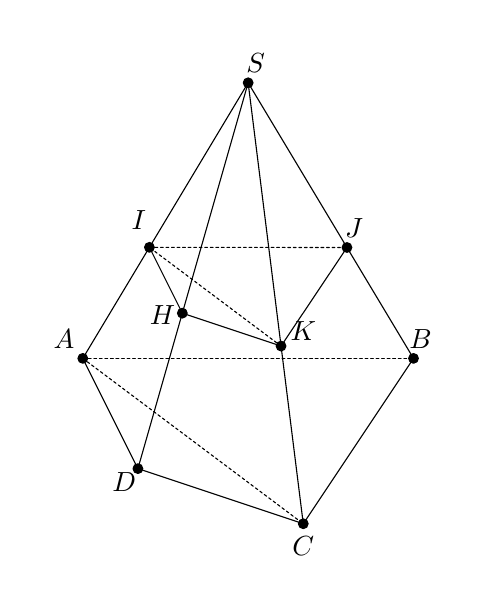
\begin{tikzpicture}[line cap=round,line join=round,>=stealth,x=1cm,y=1cm,scale=0.7]
				\clip(-1,-4) rectangle (7,6);
				\draw [dash pattern=on 1pt off 1pt] (0,0)-- (6,0);
				\draw (0,0)-- (1,-2);
				\draw (1,-2)-- (4,-3);
				\draw (4,-3)-- (6,0);
				\draw [dash pattern=on 1pt off 1pt] (0,0)-- (4,-3);
				\draw (0,0)-- (3,5);
				\draw (3,5)-- (1,-2);
				\draw (3,5)-- (4,-3);
				\draw (3,5)-- (6,0);
				\draw [dash pattern=on 1pt off 1pt] (1.2088235294117649,2.014705882352941)-- (4.792941176470588,2.011764705882353);
				\draw (1.2088235294117649,2.014705882352941)-- (1.8058823529411765,0.8205882352941177);\draw (1.8058823529411765,0.8205882352941177)-- (3.597058823529412,0.22352941176470595);
				\draw (3.597058823529412,0.22352941176470595)-- (4.792941176470588,2.011764705882353);\draw [dash pattern=on 1pt off 1pt] (3.597058823529412,0.22352941176470595)-- (1.2088235294117649,2.014705882352941);
				\begin{normalsize}
					\draw [fill=black] (0,0) circle (2.5pt);
					\draw[color=black] (-0.340663814166699,0.34993065341386587) node {$A$};
					\draw [fill=black] (6,0) circle (2.5pt);
					\draw[color=black] (6.129644307841495,0.34993065341386587) node {$B$};
					\draw [fill=black] (1,-2) circle (2.5pt);
					\draw[color=black] (0.7515109583461931,-2.2481214569577066) node {$D$};
					\draw [fill=black] (4,-3) circle (2.5pt);
					\draw[color=black] (4,-3.4) node {$C$};
					\draw [fill=black] (3,5) circle (2.5pt);
					\draw[color=black] (3.1344377347379577,5.364005745404862) node {$S$};
					\draw [fill=black] (1.2088235294117649,2.014705882352941) circle (2.5pt);
					\draw[color=black] (1.0162806001675004,2.501183993211983) node {$I$};
					\draw [fill=black] (4.792941176470588,2.011764705882353) circle (2.5pt);
					\draw[color=black] (4.921632817031782,2.3687991723013297) node {$J$};
					\draw [fill=black] (3.597058823529412,0.22352941176470595) circle (2.5pt);
					\draw[color=black] (4,0.5) node {$K$};
					\draw [fill=black] (1.8058823529411765,0.8205882352941177) circle (2.5pt);
					\draw[color=black] (1.4465312681271245,0.7801813213734893) node {$H$};
				\end{normalsize}
			\end{tikzpicture}
		\end{center}
		Ta có $\dfrac{{V_{S.ABC}}}{{V_{S.IJK}}}=\dfrac{SA}{SI}\cdot\dfrac{SB}{SJ}\cdot\dfrac{SC}{SK}=8\Rightarrow {V_{S.ABC}}=8{V_{S.IJK}}$.\\
		$\dfrac{{V_{S.ACD}}}{{V_{S.IKH}}}=\dfrac{SA}{SI}\cdot\dfrac{SC}{SK}\cdot\dfrac{SD}{SH}=8\Rightarrow {V_{S.ACD}}=8{V_{S.IKH}}$.\\
		Do đó ${V_{S.ABCD}}=8{V_{S.IJKH}}=8$.}
\end{ex}
% Cau 3 
\begin{ex}%[2H1K3-2]
	Cho hình chóp tứ giác đều $S.ABCD$ có đáy $ABCD$ là hình vuông cạnh $2a$. Mặt bên tạo với đáy góc $60^\circ$. Gọi $K$ là hình chiếu vuông góc của $O$ trên $SD$. Tính theo $a$ thể tích khối tứ diện $DKAC$.
	\choice
	{\True  $V=\dfrac{4a^3\sqrt{3}}{15}$}
	{ $V=\dfrac{4a^3\sqrt{3}}{5}$}
	{ $V=\dfrac{2a^3\sqrt{3}}{15}$}
	{ $V=a^3\sqrt{3}$}
	\loigiai{
		\begin{center}
			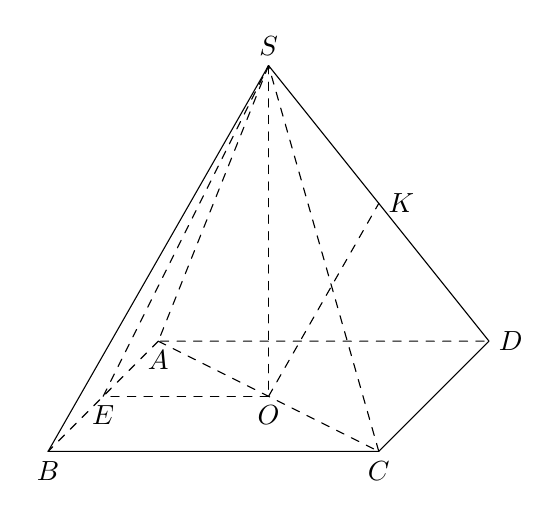
\begin{tikzpicture}[line cap=round,line join=round,>=stealth,x=1cm,y=1cm,scale=0.7]
				\draw[-](4,7)--(8,2)--(6,0) node[below]{$C$}--(0,0)--(4,7);
				\draw[dashed] (4,7)--(2,2) node[below]{$A$}--(8,2) node[right]{$D$};
				\draw[dashed] (2,2)--(0,0) node[below]{$B$};
				\draw[dashed] (6,0)--(4,7) node(S)[above]{$S$};
				\draw[dashed] (2,2)--(6,0);
				\draw[dashed] (4,7)--(4,1) node(O)[below] {$O$};
				\draw[dashed](4,1)--(1,1) node[below]{$E$};;
				\draw[dashed](1,1)--(4,7);
				\draw[dashed](4,1)--(6,4.5) node(K)[right]{$K$};
				
			\end{tikzpicture}
		\end{center}
		\begin{itemize}
			\item Gọi $E$ là trung điểm của $AB$, $O$ là tâm của hình vuông $ABCD$.\\
			$\Rightarrow OE\perp AB$,
			$SO\perp AB$
			$\Rightarrow AB\perp \left( SOE \right)$.\\
			$\Rightarrow $ góc giữa mặt bên $\left( SAB \right)$ và mặt đáy $\left( ABCD \right)$ là $\widehat{SEO}\Rightarrow \widehat{SEO}={60}^\circ$.
			\item Xét tam giác $SEO$ ta có $\tan {{60}^\circ}=\dfrac{SO}{OE}\Rightarrow SO=OE.\tan {{60}^\circ}=a\sqrt{3}$.
			\item Xét tam giác $SOD$ có đường cao $OK\Rightarrow SO^2=SK.SD\Rightarrow  \dfrac{SO^2}{SD^2}=\dfrac{SK}{SD}=\dfrac{{{\left( a\sqrt{3} \right)}^2}}{3a^2+2a^2}=\dfrac{3}{5}$.\\
			$\Rightarrow \dfrac{KD}{SD}=\dfrac{2}{5}.$
			\item $\dfrac{\mathrm{d}\left( K,\left( ABCD \right) \right)}{\mathrm{d}\left( S,\left( ABCD \right) \right)}=\dfrac{KD}{SD}=\dfrac{2}{5}\Rightarrow \mathrm{d}\left( K,\left( ABCD \right) \right)=\dfrac{2}{5}SO=\dfrac{2a\sqrt{3}}{5}.$
			\item 	Vậy ${V_{DKAC}}=\dfrac{1}{3}d\left( K,\left( ABCD \right) \right).{S_{\Delta ACD}}=\dfrac{1}{3}\cdot\dfrac{2a\sqrt{3}}{5}\cdot\dfrac{{{\left( 2a \right)}^2}}{2}=\dfrac{4a^3\sqrt{3}}{15}$.
		\end{itemize}
	}	
\end{ex}
\begin{ex}%[2H1K3-3]
	[Chuyên - KHTN - Hà Nội - 2019] 
	Cho khối chóp $S.ABCD$ có thể tích bằng $32$. Gọi $M$, $N$, $P$, $Q$ lần lượt là trung điểm $SA$, $SB$, $SC$, $SD$. Thể tích khối chóp $S.MNPQ$ bằng
	\choice
	{ $16$}
	{ $8$}
	{\True  $4$}
	{ $2$}
	\loigiai{
		\begin{center}
			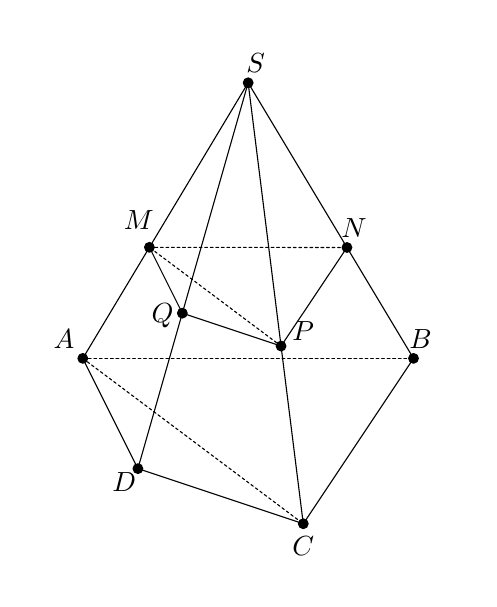
\begin{tikzpicture}[line cap=round,line join=round,>=stealth,x=1cm,y=1cm,scale=0.7]
				\clip(-1,-4) rectangle (7,6);
				\draw [dash pattern=on 1pt off 1pt] (0,0)-- (6,0);
				\draw (0,0)-- (1,-2);
				\draw (1,-2)-- (4,-3);
				\draw (4,-3)-- (6,0);
				\draw [dash pattern=on 1pt off 1pt] (0,0)-- (4,-3);
				\draw (0,0)-- (3,5);
				\draw (3,5)-- (1,-2);
				\draw (3,5)-- (4,-3);
				\draw (3,5)-- (6,0);
				\draw [dash pattern=on 1pt off 1pt] (1.2088235294117649,2.014705882352941)-- (4.792941176470588,2.011764705882353);
				\draw (1.2088235294117649,2.014705882352941)-- (1.8058823529411765,0.8205882352941177);\draw (1.8058823529411765,0.8205882352941177)-- (3.597058823529412,0.22352941176470595);
				\draw (3.597058823529412,0.22352941176470595)-- (4.792941176470588,2.011764705882353);\draw [dash pattern=on 1pt off 1pt] (3.597058823529412,0.22352941176470595)-- (1.2088235294117649,2.014705882352941);
				\begin{normalsize}
					\draw [fill=black] (0,0) circle (2.5pt);
					\draw[color=black] (-0.340663814166699,0.34993065341386587) node {$A$};
					\draw [fill=black] (6,0) circle (2.5pt);
					\draw[color=black] (6.129644307841495,0.34993065341386587) node {$B$};
					\draw [fill=black] (1,-2) circle (2.5pt);
					\draw[color=black] (0.7515109583461931,-2.2481214569577066) node {$D$};
					\draw [fill=black] (4,-3) circle (2.5pt);
					\draw[color=black] (4,-3.4) node {$C$};
					\draw [fill=black] (3,5) circle (2.5pt);
					\draw[color=black] (3.1344377347379577,5.364005745404862) node {$S$};
					\draw [fill=black] (1.2088235294117649,2.014705882352941) circle (2.5pt);
					\draw[color=black] (1.0162806001675004,2.501183993211983) node {$M$};
					\draw [fill=black] (4.792941176470588,2.011764705882353) circle (2.5pt);
					\draw[color=black] (4.921632817031782,2.3687991723013297) node {$N$};
					\draw [fill=black] (3.597058823529412,0.22352941176470595) circle (2.5pt);
					\draw[color=black] (4,0.5) node {$P$};
					\draw [fill=black] (1.8058823529411765,0.8205882352941177) circle (2.5pt);
					\draw[color=black] (1.4465312681271245,0.7801813213734893) node {$Q$};
				\end{normalsize}
			\end{tikzpicture}
		\end{center}
		Ta có $\dfrac{{V_{S.MNP}}}{{V_{S.ABC}}}=\dfrac{SM}{SA}\cdot\dfrac{SN}{SB}\cdot\dfrac{SP}{SC}=\dfrac{1}{8}$ $\Rightarrow $ ${V_{S.MNP}}=\dfrac{1}{8}{V_{S.ABC}}$.\\
		$\dfrac{{V_{S.MPQ}}}{{V_{S.ACD}}}=\dfrac{SM}{SA}\cdot\dfrac{SP}{SC}\cdot\dfrac{SQ}{SD}=\dfrac{1}{8}$ $\Rightarrow $ ${V_{S.MPQ}}=\dfrac{1}{8}{V_{S.ACD}}$.\\
		Do đó ${V_{S.MNPQ}}={V_{S.MNP}}+{V_{S.MPQ}}=\dfrac{1}{8}\left( {V_{S.ABC}}+{V_{S.ACD}} \right)=\dfrac{1}{8}{V_{S.ABCD}}=4.$\\
		Vậy ${V_{S.MNPQ}}=4$.}
\end{ex}
%Câu 5
\begin{ex}%[2H1K3-3]
	Cho hình chóp $S.ABCD$ có đáy $ABCD$ là hình thoi. Gọi $D'$ là trung điểm $SD$, mặt phẳng chứa $BD'$ và song song với $AC$ lần lượt cắt các cạnh $SA$, $SC$ tại $A'$ và $C'$. Biết thể tích khối chóp $S.A'BC'D'$ bằng $1$, tính thể tích $V$ của khối chóp $S.ABCD$.
	\choice
	{ $V=\dfrac{9}{2}$}
	{ $V=\dfrac{3}{2}$}
	{ $V=6$}
	{\True  $V=3$}
	\loigiai{
		\begin{center}
			\begin{tikzpicture}[line cap=round,line join=round,>=stealth,x=1cm,y=1cm,scale=0.7]
				\draw[-](1,7)--(8,2)--(6,0) node[below]{$D$}--(0,0)--(1,7);
				\draw[dashed] (1,7)--(2,2) node[below]{$B$}--(8,2) node[right]{$C$};
				\draw[dashed] (2,2)--(0,0) node[below]{$A$};
				\draw[dashed] (6,0)--(1,7) node(S)[above]{$S$};
				\draw[dashed] (2,2)--(6,0);
				\draw[dashed] (0,0)--(8,2);
				\node[below] at(4,1) {$O$};
				\coordinate (A1) at ($(S)!2/3!(A)$);
				\coordinate (B) at (2,2);
				\coordinate (D) at (6,0);
				\coordinate(C) at(8,2);
				\coordinate (S) at (1,7);
				\coordinate(O) at (4,1);
				\draw (A1) circle circle (0.04) node[left]{$A'$};
				\coordinate (C1) at ($(S)!2/3!(8,2)$);
				\draw (C1) circle circle (0.04) node[right]{$C'$};
				\coordinate (D1) at ($(S)!1/2!(6,0)$);
				\draw (D1) circle circle (0.04) node[above]{$D'$};
				\draw[dashed] (B)--(A1);
				\draw[dashed] (B)--(C1);
				\draw (A1)--(D1);
				\draw (D1)--(C1);
				\draw[dashed](A1)--(C1); \draw[dashed] (B)--(D1); \draw[dashed](S)--(O);
				\node[above left] at (intersection of  S--O and C1--A1){I};
			\end{tikzpicture}
		\end{center}
		Gọi $O$ là tâm hình bình hành đáy và $\left\{ I \right\}=SO\cap BD'$.\\
		Mặt phẳng được nói đến đi qua $I$ và song song $AC$ nên cắt $\left( SAC \right)$ theo giao tuyến là đường thẳng $A'C'$ qua $I$ và song song $AC$ (với $A'\in SA$, $C'\in SC$).\\
		$I$ là trọng tâm tam giác $SBD$ nên $\dfrac{SA'}{SA}=\dfrac{SC'}{SC}=\dfrac{SI}{SO}=\dfrac{2}{3}$.\\
		Ta có
		$\heva{& \dfrac{{V_{S.A'BD'}}}{{V_{S.ABD}}}=\dfrac{S{A}'}{SA}\cdot\dfrac{S{D}'}{SD}=\dfrac{2}{3}\cdot\dfrac{1}{2}=\dfrac{1}{3}. \\ &\dfrac{{V_{S.B{C}'{D}'}}}{{V_{S.BCD}}}=\dfrac{S{C}'}{SC}\cdot\dfrac{S{D}'}{SD}=\dfrac{2}{3}\cdot\dfrac{1}{2}=\dfrac{1}{3}.}$ $\Leftrightarrow \left\{ \begin{aligned}
			& {V_{S.{A}'B{D}'}}=\dfrac{1}{6}V. \\
			& {V_{S.B{C}'{D}'}}=\dfrac{1}{6}V. \\
		\end{aligned} \right.\\\Rightarrow {V_{S.A{B}'{C}'{D}'}}={V_{S.{A}'B{D}'}}+{V_{S.B{C}'{D}'}}=\dfrac{1}{3}V$
		$\Rightarrow V=3{V_{S.A{B}'{C}'{D}'}}=3$.}
\end{ex}
% Cau 6 
\begin{ex}%[2H1K3-3]
	Cho tứ diện $ABCD$ có thể tích bằng $1$. Gọi $M$, $N$, $P$ lần lượt là trọng tâm của tam giác	$ABC$, $ACD$, $ABD$. Tính thể tích của tứ diện $AMNP$.
	\choice
	{ $\dfrac{1}{27}$}
	{ $\dfrac{2}{9}$}
	{ $\dfrac{1}{3}$}
	{\True  $\dfrac{2}{27}$}
	\loigiai{
		\begin{center}
			\begin{tikzpicture}[line cap=round,line join=round,>=stealth,x=1cm,y=1cm,scale=0.7]
				\coordinate(A)  at(3,7);
				\coordinate(B) at(0,2);
				\coordinate (C) at (2,0);
				\coordinate (D) at (6,2);
				\draw [-] (A)--(B)--(C)--(D)--(A)--(C);
				\node [above] at (A) {$A$};
				\node [left] at (B) {$B$}; \node [right] at(D) {$D$}; \node[below] at(C){$C$};
				\coordinate (G) at ($(B)!.5!(D)$);
				\node [below] at (G) {$G$};
				\draw[dashed] (A)--(G);
				\draw[dashed] (B)--(D);
				\coordinate (E) at ($(B)!.5!(C)$);
				\coordinate (F) at ($(D)!.5!(C)$);
				\node [below] at (E) {$E$}; \node [below] at (F) {$F$};
				\draw[dashed] (E)--(F); \draw (A)--(E); \draw (A)--(F);
				\coordinate (M) at ($(A)!2/3!(E)$);
				\coordinate (N) at ($(A)!2/3!(F)$);
				\draw (M) circle circle (0.04) node[left]{$M$};
				\draw (N) circle circle (0.04) node[right]{$N$};
				\draw[dashed] (M)--(N);
				\coordinate (P) at ($(A)!2/3!(G)$);
				\draw[dashed] (M)--(P); \draw[dashed] (P)--(N);
				\draw[dashed] (E)--(G)--(F);
				\draw (P) circle circle (0.04) node[above right]{$P$};
			\end{tikzpicture}
		\end{center}
		Gọi $E$, $F$, $G$ lần lượt là trung điểm của $BC$, $CD$ và $DB$.\\
		Ta có ${S_{\Delta EFG}}=\dfrac{1}{4}{S_{\Delta BCD}}$ $\Rightarrow {V_{A.GEF}}=\dfrac{1}{4}{V_{A.BCD}}=\dfrac{1}{4}$.\\
		$\dfrac{{V_{AMNP}}}{{V_{AEFG}}}=\dfrac{AM}{AE}\cdot\dfrac{AN}{AF}\cdot\dfrac{AP}{AG}=\dfrac{2}{3}\cdot\dfrac{2}{3}\cdot\dfrac{2}{3}=\dfrac{8}{27}$ $\Rightarrow {V_{AMNP}}=\dfrac{8}{27}{V_{AEFG}}=\dfrac{2}{27}$.\\}
\end{ex}
% Cau 7
\begin{ex}%[2H1K3-3]
	[Sở Cần Thơ - 2019]
	Cho khối chóp $S.ABCD$ có thể tích bằng $ 18 $, đáy $ABCD$ là hình bình hành. Điểm $M$ thuộc cạnh $SD$ sao cho $SM=2MD$. Mặt phẳng $\left( ABM \right)$ cắt đường thẳng $SC$ tại $N$. Thể tích khối chóp $S.ABNM$ bằng
	\choice
	{ $ 6 $}
	{\True  $ 10 $}
	{ $ 12 $}
	{ $ 8 $}
	\loigiai{
		\begin{center}
			\begin{tikzpicture}[line cap=round,line join=round,>=stealth,x=1cm,y=1cm,scale=0.7]
				\coordinate(S)  at(4,7);
				\coordinate(A) at(0,2);
				\coordinate (D) at (6,2);
				\coordinate (B) at (2,0);
				\coordinate(C) at (8,0);
				\draw (S)--(A)--(B)--(C)--(S);
				\draw[dashed](S)--(D)--(A);
				\draw[dashed](B)--(D)--(C);
				\coordinate (M) at ($(S)!2/3!(D)$);
				\coordinate (N) at ($(S)!2/3!(C)$);
				\draw[dashed](N)--(M)--(A);
				\draw (B)--(N);
				\node[above] at(S){$S$};
				\node [left] at(A) {$A$};
				\node [below] at(D) {$D$};
				\node[below] at(B){$B$};
				\node[below] at(C){$C$};
				\node[above left] at(M){$M$}; \node[right] at(N){$N$};
				\draw[dashed](B)--(M);
				\draw(S)--(B);
			\end{tikzpicture}
		\end{center}
		Mặt phẳng $\left( MAB \right)$ và mặt phẳng $\left( SCD \right)$ có chung điểm $M$ và lần lượt chứa hai đường thẳng song song $AB$ và $CD$ nên $MN\parallel AB\parallel CD$.\\
		Vì $ABCD$ là hình bình hành nên ${V_{S.ABD}}={V_{S.BDC}}=\dfrac{1}{2}{V_{S.ABCD}}=9$.\\
		Ta có
		\begin{itemize}
			\item $\dfrac{{V_{M.ABD}}}{{V_{S.ABD}}}=\dfrac{\mathrm{d}\left( M,\left( ABD \right) \right)}{\mathrm{d}\left( S,\left( ABD \right) \right)}=\dfrac{MD}{SD}=\dfrac{1}{3}\Rightarrow {V_{M.ABD}}=3\Rightarrow {V_{S.ABM}}=6$.
			\item $\dfrac{{V_{S.BMN}}}{{V_{S.BDC}}}=\dfrac{{V_{B.SMN}}}{{V_{B.SDC}}}=\dfrac{SM.SN}{SD.SC}=\dfrac{2}{3}.\dfrac{2}{3}=\dfrac{4}{9}\Rightarrow {V_{S.BMN}}=4$.
		\end{itemize}
		$\Rightarrow {V_{S.ABNM}}={V_{S.ABM}}+{V_{S.BMN}}=6+4=10$.\\
		\textbf{Chú ý:} Có thể áp dụng công thức tỉ số thế tích và tính như sau:\\
		Ta có
		\begin{itemize}
			\item $\dfrac{{V_{S.ABM}}}{{V_{S.ABD}}}=\dfrac{SM}{SD}=\dfrac{2}{3}\Rightarrow {V_{S.ABM}}=\dfrac{2}{3}.{V_{S.ABD}}=6$.
			\item $\dfrac{{V_{S.BMN}}}{{V_{S.BDC}}}=\dfrac{SM}{SD}\cdot\dfrac{SN}{SC}=\dfrac{2}{3}\cdot\dfrac{2}{3}=\dfrac{4}{9}\Rightarrow {V_{S.BMN}}=\dfrac{4}{9}.{V_{S.BDC}}=4$.
		\end{itemize}
		$\Rightarrow {V_{S.ABNM}}={V_{S.ABM}}+{V_{S.BMN}}=6+4=10$.}
\end{ex}
% Cau 8
\begin{ex}%[2H1G3-3]
	Cho khối lăng trụ $ABC.{A}'{B}'{C}'$. Điểm $M$ thuộc cạnh ${A}'{B}'$ sao cho ${A}'{B}'=3{A}'M$. Đường thẳng $BM$ cắt đường thẳng $A{A}'$ tại $F$, và đường thẳng $CF$ cắt đường thẳng ${A}'{C}'$ tại $G$, Tính tỉ số thể tích khối chóp $F{A}'MG$ và thể tích khối đa diện lồi $GM{B}'{C}'CB$.
	\choice
	{ $\dfrac{1}{11}$}
	{ $\dfrac{1}{27}$}
	{ $\dfrac{3}{22}$}
	{\True  $\dfrac{1}{28}$}
	\loigiai{
		\begin{center}
			\begin{tikzpicture}[line cap=round,line join=round,>=stealth,x=1cm,y=1cm,scale=0.7]
				\coordinate(A) at(0,2);
				\coordinate(C) at(2,0);
				\coordinate(B) at(6,2);
				\coordinate(A') at(0,7);
				\coordinate(C') at(2,5);
				\coordinate(B') at(6,7);
				\coordinate (M) at ($(A')!1/3!(B')$);
				\draw (M) circle(0.05) node[above right]{$M$};
				\coordinate (G) at ($(A')!1/3!(C')$);
				\draw[-](A') node[left]{$A'$}--(A) node[below]{$A$}--(C)--(B) node[below] {$B$}--(B') node[right]{$B'$}--(C') node[below right]{$C'$}--(A');
				\draw[dashed](A')--(M);
				\draw(M)--(B');
				\draw(C')--(C) node[below]{$C$};
				\draw[dashed](A)--(B);
				\draw (G) circle(0.05) node[below left]{$G$};
				\draw[-](G)--(M);
				\draw[-] (C)--(G);
				\coordinate (F) at (intersection of A--A' and C--G);
				\draw(A)--(F) node[right]{$F$};
				\draw(C)--(F)--(M);
				\draw[dashed](M)--(B);
				
			\end{tikzpicture}
		\end{center}
		Ta có $GM \parallel C'B' \Rightarrow$ $\dfrac{GM}{{C}'{B}'}=\dfrac{{A}'M}{{A}'{B}'}=\dfrac{1}{3}\Rightarrow {S_{{A}'MG}}=\dfrac{1}{9}{S_{ABC}}$.\\
		Gọi $h$ là chiều cao của lăng trụ $ABC.{A}'{B}'{C}'$, $V$ là thể tích của khối lăng trụ $ABC.{A}'{B}'{C}'$.\\
		Ta có\\
		$\begin{aligned}
			{V_{{A}'MG.ABC}}&=\dfrac{h}{3}\left( {S_{ABC}}+{S_{{A}'MG}}+\sqrt{{S_{ABC}}.{S_{{A}'MG}}} \right) \\
			& =\dfrac{h}{3}\left( {S_{ABC}}+\dfrac{1}{9}{S_{ABC}}+\sqrt{{S_{ABC}}.\dfrac{1}{9}{S_{ABC}}} \right)\\
			&=\dfrac{13}{27}{S_{ABC}}.h=\dfrac{13}{27}V.\\
		\end{aligned}$\\
		$\Rightarrow {V_{GM{B}'{C}'CB}}=V-{V_{{A}'MG.ABC}}=\dfrac{14}{27}V$.\\
		Mặt khác ta cũng có\\
		$$\dfrac{FG}{FC}=\dfrac{GM}{CB}=\dfrac{1}{3}\Rightarrow \dfrac{F{A}'}{FA}=\dfrac{FG}{FC}=\dfrac{FM}{FB}=\dfrac{1}{3}\Rightarrow \dfrac{{V_{F{A}'GM}}}{{V_{FACB}}}=\dfrac{F{A}'}{FA}\cdot\dfrac{FG}{FC}\cdot\dfrac{FM}{FB}=\dfrac{1}{27}.
		$$ 
		$\Rightarrow {V_{F{A}'GM}}=\dfrac{1}{27}{V_{FACB}}=\dfrac{1}{27}\left( {V_{{A}'MG.ABC}}+{V_{F{A}'GM}} \right)$ \\
		$\Rightarrow {V_{F{A}'GM}}=\dfrac{1}{26}{V_{{A}'MG.ABC}}=\dfrac{1}{54}V$.\\
		Vậy $\dfrac{{V_{F{A}'GM}}}{{V_{{A}'MG.ABC}}}=\dfrac{1}{28}$.}
\end{ex}
% Cau 8
\begin{ex}%[2H1K3-2]
	[Sở Nam Định 2019]
	Cho tứ diện $ABCD$ có thể tích bằng $V$, hai điểm $M$ và $P$ lần lượt là trung điểm của $AB$, $CD$; điểm $N$ thuộc đoạn $AD$ sao cho $AD=3AN$. Tính thể tích tứ diện $BMNP$.
	\choice
	{ $\dfrac{V}{4}$}
	{\True  $\dfrac{V}{12}$}
	{ $\dfrac{V}{8}$}
	{ $\dfrac{V}{6}$}
	\loigiai{
		\begin{center}
			\begin{tikzpicture}[line cap=round,line join=round,>=stealth,x=1cm,y=1cm,scale=0.7]
				\coordinate(A) at (4,6);
				\coordinate(B) at (0,2);
				\coordinate(C) at (2,0);
				\coordinate(D) at (6,2);
				\draw (A) node [above]{$A$}--(B) node[left]{$B$}--(C)--(D) node[right]{$D$}--(A)--(C) node[below]{$C$};
				\draw[dashed](B)--(D);
				\coordinate (M) at ($(A)!1/2!(B)$);
				\draw (M) circle(0.05) node[above left]{$M$};
				\coordinate (P) at ($(C)!1/2!(D)$);
				\draw (P) circle(0.05) node[below right]{$P$};
				\coordinate (N) at ($(A)!1/3!(D)$);
				\draw (N) circle(0.05) node[below right]{$N$};
				\draw[dashed] (N)--(M)--(P)--(B);
				\draw(N)--(P);
			\end{tikzpicture}
		\end{center}
		Ta có
		$MB=\dfrac{AB}{2}$, $AN=\dfrac{AD}{3}\Rightarrow \mathrm{d}\left( N,AB \right)=\dfrac{1}{3}\mathrm{d}\left( D,AB \right)\Rightarrow {S_{\Delta NMB}}=\dfrac{1}{6}{S_{\Delta DAB}}
		DP=\dfrac{CD}{2}.$\\
		Ta suy ra  $\mathrm{d}\left( P,\left( MNB \right) \right)=\dfrac{1}{2}\mathrm{d}\left( C,\left( ABD \right) \right).$\\
		Dẫn đến, ${V_{P.MNB}}=\dfrac{1}{3}\mathrm{d}\left( P,\left( MNB \right) \right)\text{.}{{\text{S}}_{\Delta MNB}}=\dfrac{1}{3}.\dfrac{1}{2}\mathrm{d}\left( C,\left( ABD \right) \right).\dfrac{1}{6}{{\text{S}}_{\Delta ABD}}=\dfrac{1}{12}V.$}
\end{ex}
% Cau 10		
\begin{ex}%[2H1K3-3]
	[Nguyễn Huệ- Ninh Bình 2019]
	Cho hình chóp $S.ABCD$ có thể tích bằng $48$ và $ABCD$ là hình thoi. Các điểm $M$, $N$, $P$, $Q$ lần lượt là các điểm trên các đoạn $SA$, $SB$, $SC$, $SD$ thỏa mãn $SA=2SM$, $SB=3SN$, $SC=4SP$, $SD=5SQ$. Tính thể tích khối đa diện $S.MNPQ$.
	\choice
	{ $\dfrac{2}{5}$}
	{ $\dfrac{4}{5}$}
	{ $\dfrac{6}{5}$}
	{\True  $\dfrac{8}{5}$}
	\loigiai{
		\begin{center}
			\begin{tikzpicture}[line cap=round,line join=round,>=stealth,x=1cm,y=1cm,scale=0.7]
				\coordinate (A) at (2,2);
				\coordinate (D) at (0,0);
				\coordinate (B) at (8,2);
				\coordinate (C) at (6,0);
				\coordinate (S) at (4,7);
				\draw (S) node[above] {$S$} -- (D) node[below]{$D$} -- (C) node[below]{$C$}--(B) node [right]{$B$}--(S)--(C);
				\draw[dashed](S)--(A) node[below]{$A$}--(B);
				\draw[dashed](A)--(D);
				\coordinate (M) at ($(S)!1/2!(A)$);
				\draw (M) circle(0.05) node[below right]{$M$};
				\coordinate (N) at ($(S)!1/3!(B)$);
				\draw (N) circle(0.05) node[below right]{$N$};
				\coordinate (P) at ($(S)!1/4!(C)$);
				\draw (P) circle(0.05) node[below right]{$P$};
				\coordinate (Q) at ($(S)!1/5!(D)$);
				\draw (Q) circle(0.05) node[above left]{$Q$};
				\draw(N)--(P)--(Q);
				\draw[dashed](Q)--(M)--(N);
				\draw[dashed](M)--(P);
			\end{tikzpicture}
		\end{center}
		Ta có $ABCD$ là hình thoi nên ${S_{\Delta ACD}}={S_{\Delta ABC}}$.\\
		Suy ra ${V_{S.ACD}}={V_{S.ABC}}=\dfrac{1}{2}{V_{S.ABCD}}=24$.
		\begin{itemize}
			\item $\dfrac{{V_{S.MPQ}}}{{V_{S.ACD}}}=\dfrac{SM}{SA}\cdot\dfrac{SP}{SC}\cdot\dfrac{SQ}{SD}=\dfrac{1}{2}\cdot\dfrac{1}{4}\cdot\dfrac{1}{5}\Rightarrow {V_{S.MPQ}}=\dfrac{3}{5}$.
			\item $\dfrac{{V_{S.MNP}}}{{V_{S.ABC}}}=\dfrac{SM}{SA}\cdot\dfrac{SN}{SB}\cdot\dfrac{SP}{SC}=\dfrac{1}{2}\cdot\dfrac{1}{3}\cdot\dfrac{1}{4}\Rightarrow {V_{SMNP}}=1$.
		\end{itemize}
		Vậy ${V_{S.MNPQ}}={V_{S.MPQ}}+{V_{S.MNP}}=\dfrac{8}{5}$.}
\end{ex}
% Cau 11 
\begin{ex}%[2H1K3-3]
	Cho khối chóp đều $S.ABC$ có cạnh đáy bằng $a$, cạnh bên bằng $2a$. Gọi $M$ là trung điểm $SB$, $N$ là điểm trên đoạn $SC$ sao cho $NS=2NC$. Thể tích của khối chóp $A.BCNM$ bằng
	\choice
	{\True  $\dfrac{a^3\sqrt{11}}{18}$}
	{ $\dfrac{a^3\sqrt{11}}{24}$}
	{ $\dfrac{a^3\sqrt{11}}{36}$}
	{ $\dfrac{a^3\sqrt{11}}{16}$}
	\loigiai{
		\begin{center}
			\begin{tikzpicture}[line cap=round,line join=round,>=stealth,x=1cm,y=1cm,scale=0.7]
				\coordinate(S) at(3,7);
				\coordinate (A) at (0,3);
				\coordinate (B) at (2,2);
				\coordinate (C) at (7,4);
				\draw(S)--(A)--(B) node[below]{$B$}--(C)--(S) node[above]{$S$};
				\coordinate(O) at (3,3);
				\draw(S)--(B);
				\draw[dashed](A) node [left]{$A$}--(C) node[right]{$C$};
				\coordinate (M) at ($(S)!1/2!(B)$);
				\coordinate (I) at ($(C)!1/2!(A)$);
				\coordinate (N) at ($(S)!2/3!(C)$);
				\draw (N) circle(0.05) node[above right]{$N$};
				\draw[dashed] (B)--(I);
				\draw (O) circle(0.05) node[right]{$O$};
				\draw[dashed](S)--(I);
				\draw[dashed](S)--(O);
				\draw (A)--(M)--(N);
				\draw[dashed](N)--(A);
				\draw (I) circle(0.05) node[above left]{$I$};
				\draw (M) circle(0.05) node[above left]{$M$};
			\end{tikzpicture}
		\end{center}
		Gọi $O$ là trọng tâm của tam giác $ABC$. Khi đó $BO=\dfrac{2}{3}BI=\dfrac{2}{3}\dfrac{a\sqrt{3}}{2}=\dfrac{a\sqrt{3}}{3}$.\\
		Khối chóp $S.ABC$ đều và $O$ là trọng tâm tam giác $ABC$ lên $SO\perp \left( ABC \right)\Rightarrow SO\perp OB$\\
		$\Rightarrow \Delta SOB$ vuông tại $O$ $\Rightarrow SO=\sqrt{SB^2-OB^2}=\sqrt{4a^2-\dfrac{3a^2}{9}}=\dfrac{a\sqrt{33}}{3}$.\\
		Suy ra $ {V_{S.ABC}}=\dfrac{1}{3}SO\cdot {S_{ABC}}=\dfrac{1}{3}\cdot\dfrac{a\sqrt{33}}{3}\cdot\dfrac{1}{2}a\cdot\dfrac{a\sqrt{3}}{2}=\dfrac{a^3\sqrt{11}}{12}$.\\
		Ta có $\dfrac{{V_{S.AMN}}}{{V_{S.ABC}}}=\dfrac{SM}{SB}\cdot\dfrac{SN}{SC}=\dfrac{1}{2}\cdot\dfrac{2}{3}=\dfrac{1}{3}\Rightarrow {V_{S.AMN}}=\dfrac{1}{3}{V_{S.ABC}}$.\\
		${V_{A.BCNM}}={V_{S.ABC}}-{V_{S.AMN}}={V_{S.ABC}}-\dfrac{1}{3}{V_{S.ABC}}=\dfrac{2}{3}{V_{S.ABC}}=\dfrac{2}{3}.\dfrac{a^3\sqrt{11}}{12}=\dfrac{a^3\sqrt{11}}{18}$.}
\end{ex}
% Cau 12 
\begin{ex}%[2H1K3-3]
	Cho hình chóp $S.ABC$ có $SA=2a$, $SB=3a$, $SC=4a$ và $\widehat{ASB}=\widehat{BSC}=60^\circ $, $\widehat{ASC}=90^\circ $. Tính thể tích $V$ của khối chóp $S.ABC$.
	\choice
	{ $V=\dfrac{2a^3\sqrt{2}}{9}$}
	{\True  $V=2a^3\sqrt{2}$}
	{ $V=\dfrac{4a^3\sqrt{2}}{3}$}
	{ $V=a^3\sqrt{2}$}
	\loigiai{
		\begin{center}
			\begin{tikzpicture}[line cap=round,line join=round,>=stealth,x=1cm,y=1cm,scale=0.7]
				\coordinate(B) at(0,2);
				\coordinate(C) at(2,0);
				\coordinate(A) at(8,2);
				\coordinate(S) at(6.5,10.5);
				\draw(S)--(B) node[left]{$B$}--(C)--(A)node[right]{$A$}--(S) node[above]{$S$}--(C) node[below]{$C$};
				\draw[dashed](A)--(B);
				\coordinate (A') at ($(S)!.5!(A)$);
				\coordinate (B') at ($(S)!1/3!(B)$);
				\coordinate (C') at ($(S)!1/4!(C)$);
				\draw (A') circle(0.05);
				\draw (B') circle(0.05);
				\draw (C') circle(0.05);
				\draw(B')--(C') node[above right]{$C'$}--(A');
				\draw[dashed](B') node[left]{$B'$}--(A') node[right]{$A'$};
				\coordinate (H) at ($(A')!.5!(C')$);
				\draw (H) circle(0.05) node [right]{$H$};
				\draw(S)--(H);
			\end{tikzpicture}
		\end{center}
		Trên $SA$, $SB$, $SC$ lần lượt lấy các điểm ${A}'$, ${B}'$, ${C}'$ sao cho $S{A}'=S{B}'=S{C}'=a$. Vì $SA=2a=2S{A}'$, $SB=3a=3S{B}'$, $SC=4a=4S{C}'$ nên ta suy ra
		$$\dfrac{{V_{S.{A}'{B}'{C}'}}}{{V_{S.\,ABC}}}=\dfrac{S{A}'}{SA}\cdot\dfrac{S{B}'}{SB}\cdot\dfrac{S{C}'}{SC}=\dfrac{1}{2}\cdot\dfrac{1}{3}\cdot\dfrac{1}{4}=\dfrac{1}{24}\Rightarrow {V_{S.ABC}}=24{V_{S.{A}'{B}'{C}'}}.$$
		Theo giả thiết $\widehat{ASB}=\widehat{BSC}=60{}^\circ $ và $S{A}'=S{B}'=a$ suy ra hai tam giác $S{A}'{B}'$, $S{B}'{C}'$ đều và ${A}'{B}'={B}'{C}'=a$.\\
		Vì $\widehat{ASC}=90^\circ $ và $S{A}'=S{C}'=a$ nên tam giác ${A}'SC'$ vuông cân tại $S$, do đó ${A}'{C}'=a\sqrt{2}$.\\
		Gọi $H$ là trung điểm ${A}'{C}'$ thì $SH=\dfrac{a\sqrt{2}}{2}$ và $SH\perp {A}'{C}'\,\,\,\left( 1 \right)$.\\
		Tam giác $A'{B}'{C}'$ cân tại ${B}'$ nên trung tuyến, cũng là đường cao ${B}'H=\dfrac{a\sqrt{2}}{2}$.\\
		Xét tam giác $SH{B}'$có $SH^2+H{{{B}'}^2}=\dfrac{2a^2}{4}+\dfrac{2a^2}{4}=a^2$ suy ra $SH \perp HB'$.\\
		Từ $\left( 1 \right)$, $\left( 2 \right)$ suy ra $SH\perp \left( {A}'{B}'{C}' \right)$, nên $SH$ là chiều cao khối chóp $S.A'B'C'$.\\
		Thể tích khối chóp $S.\,{A}'{B}'{C}'$ là\\
		${V_{S.\,{A}'{B}'{C}'}}=\dfrac{1}{3}SH.{S_{\Delta {A}'{B}'{C}'}}=\dfrac{1}{3}\cdot\dfrac{a\sqrt{2}}{2}\cdot\dfrac{1}{2}{A}'{C}'\cdot{B}'H=\dfrac{a\sqrt{2}}{12}\cdot a\sqrt{2}\cdot\dfrac{a\sqrt{2}}{2}=\dfrac{a^3\sqrt{2}}{12}$.\\
		Suy ra ${V_{S.ABC}}=24{V_{S.{A}'{B}'{C}'}}=24\cdot\dfrac{a^3\sqrt{2}}{12}=2a^3\sqrt{2}$.}
\end{ex}
% Cau 13
\begin{ex}%[2H1K3-3]
	[THPT Cẩm Bình Hà Tỉnh 2019]
	Cho hình chóp đều $S.ABCD$ có đáy và cạnh bên đều bằng $a\sqrt{2}$. Gọi $M$, $N$ lần lượt là trung điểm của các cạnh $SB$, $SD$. Mặt phẳng $(AMN)$ chia khối chóp thành hai phần có thể tích $V_1$, $V_2$ với $V_1<V_2$. Ta có $V_2$ bằng
	\choice
	{ $\dfrac{a^3}{18}$}
	{\True  $\dfrac{5a^3}{9}$}
	{ $\dfrac{8a^3}{15}$}
	{ $\dfrac{a^3}{9}$}
	\loigiai{
		\begin{center}
			\begin{tikzpicture}[line cap=round,line join=round,>=stealth,x=1cm,y=1cm,scale=0.7]
				\coordinate(B) at (2,2);
				\coordinate(A) at (0,0);
				\coordinate(C) at (8,2);
				\coordinate(D) at(6,0);
				\coordinate(O) at(4,1);
				\coordinate(S) at(4,7);
				\draw(S)--(A)--(D)--(C)--(S)--(D);
				\draw[dashed] (S)--(B)--(C) (B)--(A);
				\draw [dashed](B)--(D) node[right]{$D$};
				\draw[dashed] (S) node[above]{$S$}--(O) node [below]{$O$};
				\draw[dashed] (A) node[left]{$A$}--(C) node[right]{$C$};
				\coordinate (M) at ($(B)!1/2!(S)$);
				\coordinate (N) at ($(S)!1/2!(D)$);
				\draw (M) circle(0.05) node[below]{$M$};
				\draw (N) circle(0.05) node[right]{$N$};
				\coordinate (P) at ($(S)!1/3!(C)$);
				\draw[dashed] (M)--(N);
				\draw(P)--(N)--(A);
				\draw[dashed] (A)--(M)--(P);
				\draw (P) circle(0.05) node[right]{$P$};
				\coordinate (Q) at ($(S)!2/3!(C)$);
				\draw (Q) circle(0.05) node[right]{$Q$};
				\draw[dashed](O)--(Q);
			\end{tikzpicture}
		\end{center}
		Gọi $O=AC\cap BD$, $I=SO\cap MN$, $P=AI\cap SC$.\\
		Khi đó $I$ là trung điểm của $SO.$\\
		Gọi $Q$ là trung điểm của $CP\Rightarrow IP\parallel OQ\Rightarrow P$ là trung điểm của $SQ\Rightarrow SP=PQ=QC$.\\
		Ta có $$\dfrac{{V_{S.AMP}}}{{V_{S.ABC}}}=\dfrac{SM}{SB}\cdot\dfrac{SP}{SC}=\dfrac{1}{2}\cdot\dfrac{1}{3}=\dfrac{1}{6}\Rightarrow \dfrac{{V_{S.AMPN}}}{{V_{S.ABCD}}}=\dfrac{1}{6}.$$
		Suy ra ${V_1}=\dfrac{1}{6}{V_{S.ABCD}},V_2=\dfrac{5}{6}{V_{S.ABCD}}$ (vì $V_1<V_2$ ). \\
		Mặt khác $SO=\sqrt{SA^2-A{O^2}}=\sqrt{2a^2-a^2}=a.$\\
		Do đó $V_2=\dfrac{5}{6}.\dfrac{1}{3}a.2a^2=\dfrac{5}{9}{a^3}.$}
\end{ex}
% Cau 14 
\begin{ex}%[2H1K3-3]
	Cho tứ diện $ABCD$ có $AB=1$; $AC=2$; $AD=3$ và $\widehat{BAC}=\widehat{CAD}=\widehat{DAB}={{60}^\circ}$. Tính thể tích $V$ của khối tứ diện $ABCD$.
	\choice
	{\True  $V=\dfrac{\sqrt{2}}{2}$}
	{ $V=\dfrac{\sqrt{2}}{6}$}
	{ $V=\dfrac{\sqrt{3}}{4}$}
	{ $V=\dfrac{\sqrt{2}}{12}$}
	\loigiai{
		\begin{center}\begin{tikzpicture}[xscale=1,yscale=0.5, font=\footnotesize,line join=round, line cap=round, >=stealth]
				\coordinate (A) at (1.4,7);
				\coordinate (B) at (0,0);
				\coordinate (D) at (5,0);
				\coordinate (C) at (2,-3);
				\coordinate (E) at ($(A)!2/3!(C)$);
				\coordinate (F) at ($(A)!1/2!(D)$);
				\draw (D)--(A)--(B)--(C)--(D) (A)--(C) (B)--(E)--(F);
				\draw[dashed] (F)--(B)--(D);
				\foreach \d/\g in {A/90, B/180, C/-90, D/0, E/120, F/-30}
				\fill (\d) circle (1.5pt) ($(\d)+(\g:3.5mm)$)node{$\d$};
		\end{tikzpicture}\end{center}
		Do $AB<AC<AD$ nên chọn $E\in AC$, $AE=1$, $F\in AD$, $AF=1$.\\
		Ta có $\widehat{BAC}=\widehat{CAD}=\widehat{DAB}=60{}^\circ $(giả thiết)\\
		Suy ra tứ diện $ABEF$ là tứ diện đều cạnh bằng $1$. Ta có ${V_{ABEF}}=\dfrac{\sqrt{2}}{12}$.\\
		Mặt khác ta có $\dfrac{{V_{ABCD}}}{{V_{ABEF}}}=\dfrac{AB.AC.AD}{AB.AE.AF}=\dfrac{1.2.3}{1.1.1}=6$.\\
		Từ đó ${V_{ABCD}}=\dfrac{\sqrt{2}}{2}$.}
\end{ex}
% Cau 15
\begin{ex}%[2H1K3-3]
	Cho hình chóp $S.ABC$ có đáy là tam giác $ABC$ vuông cân ở $B$, $AC=a\sqrt{2}$. $SA$ vuông góc với mặt phẳng $\left( ABC \right)$ và $SA=a$. Gọi $G$ là trọng tâm của tam giác $SBC$. Một mặt phẳng đi qua hai điểm $A$, $G$ và song song với $BC$ cắt $SB$, $SC$ lần lượt tại ${B}'$ và ${C}'$. Thể tích khối chóp $S.A{B}'{C}'$ bằng
	\choice
	{\True  $\dfrac{2a^3}{27}$}
	{ $\dfrac{a^3}{9}$}
	{ $\dfrac{4a^3}{27}$}
	{ $\dfrac{2a^3}{9}$}
	\loigiai{
		\begin{center}
			\begin{tikzpicture}[xscale=1,yscale=0.5, font=\footnotesize,line join=round, line cap=round, >=stealth]
				\coordinate (A) at (0,2);
				\coordinate (S) at(0,8);
				\coordinate (B) at (8,2);
				\coordinate(C) at (2,0);
				\draw(S) node[above]{$S$}--(A) node[left]{$A$}--(C) node[below]{$C$}--(B) node[right]{$B$}--(S)--(B)--(S)--(C);	
				\draw[dashed](A)--(B);
				\coordinate (M) at ($(B)!1/2!(C)$);
				\draw (M) node[below]{$M$}--(S);
				\coordinate (N) at ($(S)!1/2!(B)$);
				\draw (C)--(N) node [right]{$N$};
				\draw (M) circle (0.05);	\draw (N) circle (0.05);
				\coordinate (G) at ($(S)!2/3!(M)$);
				\draw (G) circle (0.05) node[below]{$G$};
				\coordinate (C') at ($(S)!2/3!(C)$);
				\draw (C') circle (0.05) node[above right]{$C'$};
				\coordinate (B') at ($(S)!2/3!(B)$);
				\draw (B') circle (0.05) node[above right]{$B'$};
				\draw(B')--(C')--(A);
				\draw[dashed] (A)--(B');
			\end{tikzpicture}
		\end{center}
		Gọi $M$, $N$ lần lượt là trung điểm của đoạn thẳng $BC$, $SB$. Khi đó, $G=SM\cap CN$.\\
		Đặt $BA=BC=x>0$. Theo định lý Pitago trong tam giác $ABC$ vuông tại $B$, ta có\\
		$A{C^2}=BA^2+BC^2\Rightarrow {{\left( a\sqrt{2} \right)}^2}=x^2+x^2\Rightarrow {x^2}=a^2\Rightarrow x=a$.\\
		Diện tích tam giác $ABC$ là ${S_{ABC}}=\dfrac{1}{2}.BA.BC=\dfrac{a^2}{2}$.\\
		Thể tích khối chóp $S.ABC$ là ${V_{S.ABC}}=\dfrac{1}{3}\cdot {S_{ABC}}\cdot SA=\dfrac{1}{3}\cdot\dfrac{a^2}{2}\cdot a=\dfrac{a^3}{6}$.\\
		Mặt phẳng qua $A$, $G$ song song với $BC$ cắt $SB$, $SC$ lần lượt tại ${B}'$, ${C}'$ nên $B'C'\parallel BC$. \\Khi đó ta có $\dfrac{S{B}'}{SB}=\dfrac{S{C}'}{SC}=\dfrac{SG}{SM}=\dfrac{2}{3}$.\\
		Ta lại có $\dfrac{{V_{S.A{B}'{C}'}}}{{V_{S.ABC}}}=\dfrac{SA}{SA}\cdot\dfrac{S{B}'}{SB}\cdot\dfrac{S{C}'}{SC}=1\cdot \dfrac{2}{3}\cdot\dfrac{2}{3}=\dfrac{4}{9}$.\\
		Suy ra, ${V_{S.A{B}'{C}'}}=\dfrac{4}{9}\cdot {V_{S.ABC}}=\dfrac{4}{9}\cdot\dfrac{a^3}{6}=\dfrac{2a^3}{27}$.}
\end{ex}
% Cau 16
\begin{ex}%[2H1K3-3]
	Một viên đá có dạng khối chóp tứ giác đều với tất cả các cạnh bằng nhau và bằng $a$. Người ta cưa viên đá đó theo mặt phẳng song song với mặt đáy của khối chóp để chia viên đá thành hai phần có thể tích bằng nhau. Tính diện tích thiết diện viên đá bị cưa bởi mặt phẳng nói trên.
	\choice
	{ $\dfrac{a^2}{\sqrt[3]{2}}$}
	{ $\dfrac{a^2}{\sqrt{3}}$}
	{\True  $\dfrac{a^2}{\sqrt[3]{4}}$}
	{ $\dfrac{\sqrt[3]{2}{a^2}}{4}$}
	\loigiai{
		\begin{center}
			\begin{tikzpicture}
				\def\a{4}
				\def\h{4.5}
				\path 	(0:0) coordinate (A)
				++(0:\a) coordinate (D)
				++(-135:\a/2) coordinate (C)
				($(A)+(C)-(D)$) coordinate (B)
				(intersection of A--C and B--D) coordinate (O)
				($(O)+(90:\h)$) coordinate (S)
				($(S)!0.5!(A)$) coordinate (A')
				($(S)!0.5!(B)$) coordinate (B')
				($(S)!0.5!(C)$) coordinate (C')
				($(S)!0.5!(D)$) coordinate (D')
				;
				\draw[dashed,thick] 	(B)--(A)--(D)	(A)--(S)
				(A)--(C)	(B)--(D) (B')--(A')--(D') (A')--(C')	;
				\draw[thick] 			(B)--(C)--(D)
				(B')--(C')--(D')			(B)--(S)	(C)--(S)	(D)--(S);
				\foreach \x/\g in {A/45,B/-135,C/-45,D/45,S/90,A'/45,B'/-150,C'/-30,D'/45}
				\fill[black] 	(\x) circle (1.5pt)
				($(\g:4mm)+(\x)$) node {$\x$};	
				\node[above right] at ($(S)!0.5!(D')$) {$x$};
				\node[above] at ($(A)!0.5!(B)$) {$a$};				
			\end{tikzpicture}
		\end{center}
		Gọi khối chóp tứ giác đều là $S.ABCD$ có tất cả các cạnh bằng $a$.\\
		Vì mặt phẳng cắt hình khối chóp song song với đáy nên thiết diện tạo bởi mặt cắt và khối chóp là một hình vuông ${A}'{B}'{C}'{D}'$.\\
		Giả sử $\dfrac{S{A}'}{SA}=k$, ta có$\dfrac{S{A}'}{SA}=\dfrac{S{B}'}{SB}=\dfrac{S{C}'}{SC}=\dfrac{S{D}'}{SD}=\dfrac{{A}'{B}'}{AB}=k$ (định lí Talet).\\
		Theo giả thiết ${V_{S.{A}'{B}'{C}'{D}'}}=\dfrac{1}{2}{V_{S.ABCD}}$ $\Leftrightarrow 2{V_{S.{A}'{B}'{C}'}}=\dfrac{1}{2}\cdot2\cdot {V_{S.ABC}}$\\
		$\Leftrightarrow {V_{S.{A}'{B}'{C}'}}=\dfrac{1}{2}\cdot{V_{S.ABC}}$ $\Leftrightarrow \dfrac{{V_{S.{A}'{B}'{C}'}}}{{V_{S.ABC}}}=\dfrac{1}{2}$\\
		$\Leftrightarrow \dfrac{S{A}'}{SA}\cdot\dfrac{S{B}'}{SB}\cdot\dfrac{S{C}'}{SC}=\dfrac{1}{2}$ $\Leftrightarrow {{\left( k \right)}^3}=\dfrac{1}{2}\Leftrightarrow k=\dfrac{1}{\sqrt[3]{2}}$ $\Rightarrow \dfrac{{A}'{B}'}{AB}=\dfrac{1}{\sqrt[3]{2}}$\\
		$\Rightarrow {A}'{B}'=\dfrac{a}{\sqrt[3]{2}}\Rightarrow {S_{{A}'{B}'{C}'{D}'}}={{\left( \dfrac{a}{\sqrt[3]{2}} \right)}^2}=\dfrac{a^2}{\sqrt[3]{4}}$.}
\end{ex}
% Cau 17
\begin{ex}%[2H1K3-3]	
	[THPT Yên Dũng 2-Bắc Giang] Cho tứ diện $ABCD$ có các cạnh $AB$, $AC$, $AD$ vuông góc với nhau từng đôi một và $AB=3a$, $AC=6a$, $AD=4a$. Gọi $M$, $N$, $P$ lần lượt là trung điểm của các cạnh $BC$, $CD$, $BD$. Tính thể tích khối đa diện $AMNP$.
	\choice
	{ $12a^3$}
	{\True  $3a^3$}
	{ $2a^3$}
	{ $a^3$}
	\loigiai{
		\begin{center}			
			\begin{tikzpicture}
				\def\a{5} %Khai báo cạnh
				\def\h{4}
				\path 	(0:0) coordinate (A)
				++(0:\a) coordinate (C)
				++(-150:4*\a/5) coordinate (B)
				($(A)+(90:\h)$) coordinate (D)
				($(C)!0.5!(B)$) coordinate (M)
				($(C)!0.5!(D)$) coordinate (N)
				($(D)!0.5!(B)$) coordinate (P)
				;
				\draw[thick] 	(A)--(B)--(C)
				(A)--(D)	(B)--(D)	(C)--(D) (M)--(N)--(P)--cycle (A)--(P)--(N);
				\draw[dashed,thick] 	(A)--(C) (M)--(A)--(N);
				\foreach \x /\goc in {A/180,C/0,B/-135,D/90,M/-45,N/45,P/180}
				\fill[black] (\x) circle (1.5pt)
				($(\x)+(\goc:3mm)$) node {$\x$};				
			\end{tikzpicture}			
		\end{center}
		Ta có: $\dfrac{{V_{D.APN}}}{{V_{D.ABC}}}=\dfrac{DP}{DB}\cdot\dfrac{DN}{DC}=\dfrac{1}{4}$; $\dfrac{{V_{B.APM}}}{{V_{B.ACD}}}=\dfrac{BP}{BD}\cdot\dfrac{BM}{BC}=\dfrac{1}{4}$; $\dfrac{{V_{C.AMN}}}{{V_{C.ABD}}}=\dfrac{CM}{CB}\cdot\dfrac{CN}{CD}=\dfrac{1}{4}$.\\
		Mà ${V_{AMNP}}={V_{ABCD}}-{V_{DAPN}}-{V_{BAPM}}-{V_{CAMN}}=\dfrac{1}{4}{V_{ABCD}}=\dfrac{1}{4}\left( \dfrac{1}{6}\cdot AB\cdot AC\cdot AD \right)$\\
		$\Rightarrow {V_{AMNP}}=\dfrac{1}{4}\left( \dfrac{1}{6}\cdot 3a\cdot 6a\cdot4a \right)=3a^3$.}
\end{ex}
% Cau 18
\begin{ex}%[2H1K3-3]	
	[HKI-Chuyên Long An-2019] Cho hình chóp $S.ABCD$ có đáy $ABCD$ là hình thoi và có thể tích bằng $2$. Gọi $M$, $N$ lần lượt
	là các điểm trên cạnh $SB$ và $SD$ sao cho $\dfrac{SM}{SB}=\dfrac{SN}{SD}=k$. Tìm giá trị của $k$ để thể tích khối chóp $S.AMN$ bằng $\dfrac{1}{8}$.
	\choice
	{ $k=\dfrac{1}{8}$}
	{\True  $k=\dfrac{\sqrt{2}}{4}$}
	{ $k=\dfrac{1}{4}$}
	{ $k=\dfrac{\sqrt{2}}{2}$}
	\loigiai{
		\begin{center}			
			\begin{tikzpicture}
				\def\a{4}
				\def\h{4}
				\path 	(0:0) coordinate (A)
				++(0:\a) coordinate (D)
				++(-130:\a/2) coordinate (C)
				($(A)+(C)-(D)$) coordinate (B)
				($(A)+(90:\h)$) coordinate (S)
				(intersection of A--C and B--D) coordinate (O)
				($(S)!0.5!(B)$) coordinate (M)
				($(S)!0.5!(D)$) coordinate (N)
				;%giao điểm O
				\draw[dashed,thick] 	(B)--(A)--(D)--cycle	(A)--(S) (M)--(A)--(N)--cycle ;
				\draw[thick] 			(B)-- (C)--(D)
				(B)--(S)	(C)--(S)	(D)--(S);
				\foreach \x/\g in {A/180,B/-135,C/-45,D/45,S/90,M/150,N/45}
				\fill[black] 	(\x) circle (1.5pt)
				($(\g:3mm)+(\x)$) node {$\x$};	
				
			\end{tikzpicture}
		\end{center}
		Vì đáy $ABCD$ là hình thoi nên ${S_{\Delta ABD}}={S_{\Delta CBD}}\Rightarrow {V_{S.ABD}}=\dfrac{1}{2}{V_{S.ABCD}}=1$.\\
		Mặt khác $\dfrac{{V_{S.AMN}}}{{V_{S.ABD}}}=\dfrac{SA}{SA}\cdot\dfrac{SM}{SB}\cdot \dfrac{SN}{SD}\Leftrightarrow {V_{S.AMN}}=k^2$, Có ${V_{S.AMN}}=\dfrac{1}{8}$\\
		Suy ra $k^2=\dfrac{1}{8}\Rightarrow k=\dfrac{\sqrt{2}}{4}$ (do $k>0$). Vậy $k=\dfrac{\sqrt{2}}{4}$.}
\end{ex}
% Cau 19
\begin{ex}%[2H1K3-3]	
	[THPT Đoàn Thượng – Hải Dương] Cho hình chóp tứ giác $ S.ABCD $ có thể tích bằng $ V $. Lấy điểm ${A}'$ trên cạnh $ SA $ sao cho $SA'=\dfrac{1}{3}SA$. Mặt phẳng qua ${A}'$ và song song với đáy của hình chóp cắt các cạnh $ SB$, $SC$, $SD $ lần lượt tại $ B’$,  $C’$, $D’ $. Tính theo $ V $ thể tích khối chóp $ S.A’B’C’D’ $?
	\choice
	{ $\dfrac{V}{3}$}
	{ $\dfrac{V}{81}$}
	{\True  $\dfrac{V}{27}$}
	{ $\dfrac{V}{9}$}
	\loigiai{
		\begin{center}
			
			\begin{tikzpicture}
				\def\a{5}
				\path 	(0:0) coordinate (A)
				++(0:\a) coordinate (D)
				++(-130:\a/2) coordinate (C)
				++(-165:2*\a/4) coordinate (B)
				($(A)+(70:\a)$) coordinate (S)
				(intersection of A--C and B--D) coordinate (O)
				($(S)!0.34!(A)$) coordinate (A')
				($(S)!0.34!(B)$) coordinate (B')
				($(S)!0.34!(C)$) coordinate (C')
				($(S)!0.34!(D)$) coordinate (D')
				
				;%giao điểm O
				\draw[dashed,thick] 	(C)--(A)--(D) (D')--(A')--(C');
				\draw[thick] 			(A)--(B)--(C)--(D) (A')--(B')--(C')--(D')
				(A)--(S)	(B)--(S)	(C)--(S)	(D)--(S);
				\foreach \x/\g in {A/180,B/-135,C/-45,D/0,S/90,A'/180,B'/-135,C'/-20,D'/0}
				\fill[black] 	(\x) circle (1pt)
				($(\g:3mm)+(\x)$) node {$\x$};	
			\end{tikzpicture}
		\end{center}
		Ta có
		${V_{S.ABC}}+{V_{S.AC{D}}}={V_{S.ABC{D}}}$; $\dfrac{{V_{S.A'B'C'}}}{{V_{S.ABC}}}=\dfrac{SA'}{SA}\cdot\dfrac{SB'}{SB}\cdot\dfrac{SC'}{SC}={{\left( \dfrac{1}{3} \right)}^3}=\dfrac{1}{27}$\\
		$\dfrac{{V_{S.A'D'C'}}}{{V_{S.ADC}}}=\dfrac{SA'}{SA}\cdot\dfrac{SD'}{SD}\cdot\dfrac{SC'}{SC}={{\left( \dfrac{1}{3} \right)}^3}=\dfrac{1}{27}$; ${V_{S.A'B'C'{D }\!\!'\!\!{ }}}={V_{S.A'B'C'}}+{V_{S.A'C'{D }\!\!'\!\!{ }}}=\dfrac{1}{27}{V_{S.ABC{D}}}$.}
\end{ex}
% Cau 20
\begin{ex}%[2H1K3-3]
	[THPT Đoàn Thượng – Hải Dương]
	Cho tứ diện $ABCD$ có các cạnh $AB$, $AC$ và $AD$ đôi một vuông góc với nhau. Gọi $G_1$, $G_2$, $G_3$ và $G_4$ lần lượt là trọng tâm các tam giác $ABC$, $ABD$, $ACD$ và $BCD$. Biết $AB=6a$, $AC=9a$, $AD=12a$. Tính theo $ a $ thể tích khối tứ diện $G_1{G_2}{G_3}{G_4}$.
	\choice
	{\True  $4a^3$}
	{ $a^3$}
	{ $108a^3$}
	{ $36a^3$}
	\loigiai{
		\begin{center}			
			\begin{tikzpicture}[scale=1.2]
				\def\a{4}
				\def\b{6}
				\def\h{4}
				\path 	(0:0) coordinate (A)
				++(0:\a) coordinate (D)
				++(-160:\b) coordinate (C)
				($(A)+(90:\h)$) coordinate (B)
				($(C)!0.5!(D)$) coordinate (E)
				($(A)!0.5!(D)$) coordinate (F)
				($(A)!0.5!(C)$) coordinate (H)
				($(B)!0.67!(E)$) coordinate (G4)
				($(B)!0.67!(F)$) coordinate (G2)
				($(B)!0.67!(H)$) coordinate (G1)
				($(A)!0.67!(E)$) coordinate (G3)
				;%giao điểm O
				\draw[dashed,thick] 	(C)--(A)--(D) (E)--(A)--(B) (G1)--(G2)--(G3)--(G4)--(G1)--(G3) (G4)--(G2) (H)--(B)--(F) ;
				\draw[thick] 	(B)--(E)		(B)-- (C)--(D)--cycle
				;
				\foreach \x/\g in {A/180,B/90,C/-135,D/0,E/-45,F/-90}
				\fill[black] 	(\x) circle (1.5pt)
				($(\g:3mm)+(\x)$) node {$\x$};
				\begin{scriptsize}
					\fill[black] 	(G1) circle (1.5pt)
					($(-150:2.7mm)+(G1)$) node {$G_1$};	
					\fill[black] 	(G2) circle (1.5pt)
					($(50:2.7mm)+(G2)$) node {$G_2$};	
					\fill[black] 	(G3) circle (1.5pt)
					($(-140:2.7mm)+(G3)$) node {$G_3$};	
					\fill[black] 	(G4) circle (1.5pt)
					($(-135:2.7mm)+(G4)$) node {$G_4$};	
				\end{scriptsize}				
			\end{tikzpicture}
		\end{center}
		$\Delta {G_1}{G_2}{G_3}$ đồng dạng với $\Delta ACD$ theo tỉ số $\dfrac{1}{3}$ và nằm trong hai mặt phẳng song song.\\
		${S_{\Delta {G_1}{G_2}{G_3}}}=\dfrac{1}{9}{S_{\Delta ABD}}=6a^2$. \\
		$G_3G_4\parallel AB$ và $G_3G_4=\dfrac{1}{3}AB=2a$. 
		\\Suy ra ${V_{G_1{G_2}{G_3}{G_4}}}=\dfrac{1}{3}{G_3}{G_4}.{S_{\Delta {G_1}{G_2}{G_3}}}=4a^3.$}
\end{ex}
% Cau 21
\begin{ex}%[2H1K3-3]	
	[Chuyên Vĩnh Phúc - 2019]
	Cho hình chóp $S.ABC$ có đáy là tam giác $ABC$ vuông cân ở $B$, $AC=a\sqrt{2}$, $SA\bot \left( ABC \right)$, $SA=a$. Gọi $G$ là trọng tâm của tam giác $SBC$, mặt phẳng $\left( \alpha  \right)$ đi qua $AG$ và song song với $BC$ chia khối chóp thành hai phần. Gọi $V$ là thể tích của khối đa diện không chứa đỉnh $S$. Tính $V$.
	\choice
	{ $\dfrac{4a^3}{9}$}
	{ $\dfrac{4a^3}{27}$}
	{\True  $\dfrac{5a^3}{54}$}
	{ $\dfrac{2a^3}{9}$}
	\loigiai{
		\begin{center}
			
			\begin{tikzpicture}
				\def\a{5} %Khai báo cạnh
				\def\h{4}
				\path 	(0:0) coordinate (A)
				++(0:\a) coordinate (B)
				++(-140:4*\a/5) coordinate (C)
				($(A)+(90:\h)$) coordinate (S)
				($(B)!0.5!(S)$) coordinate (N)
				($(B)!0.5!(C)$) coordinate (M)
				($(S)!0.67!(M)$) coordinate (G)
				($(S)!0.67!(C)$) coordinate (C')
				($(S)!0.67!(B)$) coordinate (B')
				;
				\draw[thick] 	(A)--(C)--(B)
				(A)--(S)	(B)--(S)	(N)--(C)--(S)--(M) (A)--(C')--(B');
				\draw[dashed,thick] 	(B')--(A)--(B);
				\foreach \x /\goc in {A/180,B/0,C/-135,S/90,M/-45,G/0,B'/45,C'/-10,N/60}
				\fill[black] (\x) circle (1.5pt)
				($(\x)+(\goc:3mm)$) node {$\x$};
				
				\draw pic[draw,angle radius=2mm]{right angle=A--B--C};%Theo chiều dương
				
			\end{tikzpicture}
		\end{center}
		Trong mặt phẳng $\left( SBC \right)$ kẻ đường thẳng qua $G$ song song với $BC$, cắt $SB$, $SC$ lần lượt tại ${B}'$, ${C}'$. Khi đó mặt phẳng $\left( \alpha  \right)$ trùng với mặt phẳng $\left( A{B}'{C}' \right)$.\\
		Gọi $M$, $N$ lần lượt là trung điểm của đoạn thẳng $BC$, $SB$.\\
		Đặt $BA=BC=x>0$. Theo định lý Pitago trong tam giác $ABC$ vuông tại $B$, ta có\\
		$A{C^2}=BA^2+BC^2\Rightarrow {{\left( a\sqrt{2} \right)}^2}=x^2+x^2\Rightarrow {x^2}=a^2\Rightarrow x=a$.\\
		Diện tích tam giác $ABC$ là ${S_{ABC}}=\dfrac{1}{2}\cdot BA\cdot BC=\dfrac{a^2}{2}$.\\
		Thể tích khối chóp $S.ABC$ là ${V_{S.ABC}}=\dfrac{1}{3}\cdot {S_{ABC}}\cdot SA=\dfrac{1}{3}\cdot\dfrac{a^2}{2}\cdot a=\dfrac{a^3}{6}$.\\
		Ta lại có $\dfrac{S{B}'}{SB}=\dfrac{S{C}'}{SC}=\dfrac{SG}{SM}=\dfrac{2}{3}$.\\
		Suy ra: $\dfrac{{V_{S.A{B}'{C}'}}}{{V_{S.ABC}}}=\dfrac{SA}{SA}\cdot\dfrac{S{B}'}{SB}\cdot\dfrac{S{C}'}{SC}=1\cdot\dfrac{2}{3}\cdot\dfrac{2}{3}=\dfrac{4}{9}$.\\
		Vì thế, ${V_{S.A{B}'{C}'}}=\dfrac{4}{9}.{V_{S.ABC}}=\dfrac{4}{9}\cdot\dfrac{a^3}{6}=\dfrac{2a^3}{27}$.\\
		Vậy $V={V_{S.ABC}}-{V_{S.A{B}'{C}'}}=\dfrac{a^3}{6}-\dfrac{2a^3}{27}=\dfrac{5a^3}{54}$.}
\end{ex}
% Cau 22
\begin{ex}%[2H1K3-3]	
	[Chuyên Lam Sơn 2019] Cho tứ diện $ABCD$ có thể tích $V$. Gọi $E$, $F$, $G$ lần lượt là trung điểm của $BC$, $BD$, $CD$ và $M$, $N$, $P$, $Q$ lần lượt là trọng tâm $\Delta ABC$, $\Delta ABD$, $\Delta ACD$, $\Delta BCD$. Tính thể tích khối tứ diện $MNPQ$ theo $V$.
	\choice
	{ $\dfrac{V}{9}$}
	{ $\dfrac{V}{3}$}
	{ $\dfrac{2V}{9}$}
	{\True  $\dfrac{V}{27}$}
	\loigiai{
		\begin{center}
			
			\begin{tikzpicture}
				\def\a{6}
				\def\b{4.5}
				\path 	(0:0) coordinate (B)
				++(0:\a) coordinate (D)
				++(-160:\b) coordinate (C)
				($(B)+(70:\b)$) coordinate (A);
				\foreach \x/\y/\t/\z in {C/B/E/0.5,B/D/F/0.5,D/C/G/0.5,A/E/M/0.67,A/F/N/0.67,A/G/P/0.67,B/G/Q/0.67}
				\coordinate (\t) at
				($(\x)!\z!(\y)$);
				\draw[dashed,thick] 	(G)--(B)--(D) (A)--(F) (M)--(N)--(P)--(Q)--(M)--(P) (Q)--(N);
				\draw[thick] 	(E)--(A)--(G)		(B)--(A)--(D) (A)--(C)
				(B)--(C)--(D);
				\foreach \x/\g in {A/90,B/180,C/-45,D/0,E/-135,F/-70,G/-40,M/180,N/170,P/10,Q/-130}
				\fill[black] 	(\x) circle (1.5pt)
				($(\g:3mm)+(\x)$) node {$\x$};
				
				%Hình chóp S.ABC có SA vuông góc đáy	
			\end{tikzpicture}
		\end{center}
		Ta có $\Delta MNP\sim \Delta EFG$ và $\dfrac{MN}{EF}=\dfrac{2}{3}$;
		$\Delta EFG\sim \Delta DCB$ và $\dfrac{EF}{DC}=\dfrac{1}{2}$.\\
		Do đó $\Delta MNP\sim \Delta DCB$ và $\dfrac{MN}{DC}=\dfrac{1}{3}\cdot\dfrac{{S_{\Delta MNP}}}{{S_{\Delta BCD}}}=\dfrac{1}{9}\Rightarrow {S_{\Delta MNP}}=\dfrac{1}{9}{S_{\Delta BCD}}$\\
		Mặt khác $\mathrm{d}\left( Q,\left( MNP \right) \right)=\dfrac{1}{3}\mathrm{d}\left( A,\left( BCD \right) \right)$\\
		Suy ra ${V_{MNPQ}}=\dfrac{1}{27}V$.}
\end{ex}
% Cau 23
\begin{ex}%[2H1K3-3]	
	[THPT QG - 2017]
	Cho tứ diện $ABCD$ có thể tích bằng $ 12 $ và $G$ là trọng tâm của tam giác $BCD$. Tính thể tích $V$ của khối chóp $A.GBC$.
	\choice
	{ $V=3$}
	{\True  $V=\,\,4$}
	{ $V=6$}
	{ $V=5$}
	\loigiai{
		Do $G$ là trọng tâm tam giác $BCD$ nên ta có ${S_{\Delta BGC}}={S_{\Delta BGD}}={S_{\Delta CGD}}$. 
		\\Khi đó, ${S_{\Delta BCD}}=3{S_{\Delta BGC}}$.\\
		Áp dụng công thức thể tích hình chóp ta có\\
		$\left. \begin{aligned}
			& {V_{ABCD}}=\dfrac{1}{3}h.{S_{\Delta BCD}} \\
			& {V_{A.GBC}}=\dfrac{1}{3}h.{S_{\Delta GBC}} \\
		\end{aligned} \right\}\Rightarrow \dfrac{{V_{ABCD}}}{{V_{A.GBC}}}=\dfrac{\dfrac{1}{3}h.{S_{\Delta BCD}}}{\dfrac{1}{3}h.{S_{\Delta GBC}}}=\dfrac{{S_{\Delta BCD}}}{{S_{\Delta GBC}}}=3$\\
		$\Rightarrow {V_{A.GBC}}=\dfrac{1}{3}{V_{ABCD}}=\dfrac{1}{3}.12=4$.
		\begin{center}			
			\begin{tikzpicture}
				\def\a{6}
				\def\b{4.5}
				\path 	(0:0) coordinate (B)
				++(0:\a) coordinate (D)
				++(-160:\b) coordinate (C)
				($(B)+(70:\b)$) coordinate (A)
				($(C)!0.5!(D)$) coordinate (M)
				($(B)!0.67!(M)$) coordinate (G);
				\draw[dashed,thick] 	(D)--(B)--(M) (A)--(G)--(C);
				\draw[thick] 			(B)--(A)--(D) (A)--(C)
				(B)--(C)--(D);
				\foreach \x/\g in {A/90,B/180,C/-45,D/0,G/40}
				\fill[black] 	(\x) circle (1.5pt)
				($(\g:3mm)+(\x)$) node {$\x$};
				%Hình chóp S.ABC có SA vuông góc đáy	
			\end{tikzpicture}
	\end{center}}
\end{ex}
% Cau 24
\begin{ex}%[2H1K3-3]	
	Cho tứ diện đều $ABCD$ có cạnh bằng $a$. Gọi $M$, $N$ lần lượt là trung điểm của các cạnh $AB$, $BC$ và $E$ là điểm đối xứng với $B$ qua $D$. Mặt phẳng $(MNE)$ chia khối tứ diện $ABCD$ thành hai khối đa diện, trong đó khối chứa điểm $A$ có thể tích $V$. Tính $V$.
	\choice
	{ $\dfrac{13\sqrt{2}{a^3}}{216}$}
	{ $\dfrac{7\sqrt{2}{a^3}}{216}$}
	{ $\dfrac{\sqrt{2}{a^3}}{18}$}
	{\True  $\dfrac{11\sqrt{2}{a^3}}{216}$}
	\loigiai{		
		\begin{center}			
			\begin{tikzpicture}
				\def\a{5}
				\def\h{4.5}
				\path 	(0:0) coordinate (B)
				++(0:\a) coordinate (D)
				++(-160:4*\a/5) coordinate (C)
				($(C)!0.5!(D)$) coordinate (F)
				($(B)!2/3!(F)$) coordinate (H)
				($(H)+(90:\h)$) coordinate (A);
				\draw[thick] (A)--(B)--(C)--(D)--(A)--(C);
				\draw[dashed,thick] (A)--(H) (D)--(B)--(F);
				\foreach \x / \goc in {B/180,D/0,C/-90,H/-90,F/-45,A/90}
				\fill (\x) circle (1.5pt)
				($(\x)+(\goc:3mm)$) node {$\x$};
			\end{tikzpicture}
		\end{center}
		\begin{center}			
			\begin{tikzpicture}
				\def\a{8}
				\def\b{4.5}
				\path 	(0:0) coordinate (B)
				++(0:\a) coordinate (E)
				++(-150:6) coordinate (C)				
				($(B)!0.5!(E)$) coordinate (D)
				($(B)!0.5!(A)$) coordinate (M)
				($(B)!0.5!(C)$) coordinate (N)
				(intersection of A--D and E--M) coordinate (Q)
				(intersection of C--D and E--N) coordinate (P)
				;
				\draw[dashed,thick] 	(B)--(E) (A)--(D)--(C) (M)--(E)--(N);
				\draw[thick] 	(M)--(N)		(B)--(A)--(E) (A)--(C)
				(B)--(C)--(E);
				\foreach \x/\g in {A/90,B/180,C/-45,E/0,D/60,M/170,N/-135,P/-45,Q/45}
				\fill[black] 	(\x) circle (1pt)
				($(\g:3mm)+(\x)$) node {$\x$};
				%Hình chóp S.ABC có SA vuông góc đáy	
			\end{tikzpicture}
		\end{center}
		Tính thể tích $T$ có khối tứ diện $ABCD$. Gọi $F$ là trung điểm $BC$ và $H$ trọng tâm tam giác $BCD$.\\
		Ta có $BF=\dfrac{a\sqrt{3}}{2}$ và $BH=\dfrac{2}{3}BF=\dfrac{a}{\sqrt{3}}$ suy ra $BH=\sqrt{A{B^2}-BH^2}=a\sqrt{\dfrac{2}{3}}$.\\
		Thể tích tứ diện $ABCD$ là $T=\dfrac{1}{3}AH\cdot{S_{BCD}}=\dfrac{1}{3}a\sqrt{\dfrac{2}{3}}\cdot\dfrac{a^2\sqrt{3}}{4}=\dfrac{a^3\sqrt{2}}{12}$.\\
		Gọi diện tích một mặt của tứ diện là$S$. Gọi $P$ là giao điểm của $NE$ và $CD$, tương tự cho $Q$.\\
		Ta thấy $P$, $Q$ lần lượt là trọng tâm các tam giác $BEC$ và $BEA$ nên $PD=\dfrac{1}{3}DC$, $QD=\dfrac{1}{3}AD$.\\
		Sử dụng công thức tỉ số thể tích ta có\\
		$\dfrac{{V_{B.ACE}}}{{V_{B.ACD}}}=2$ nên ${V_{B.ACE}}=2T$; $\dfrac{{V_{E.BMN}}}{{V_{E.BAC}}}=\dfrac{1}{4}$ nên ${V_{E.BMN}}=\dfrac{1}{4}.2T=\dfrac{T}{2}$.\\
		Nên ${V_{E.AMNC}}={V_{E.ABC}}-{V_{B.EMN}}=2T-\dfrac{T}{2}=\dfrac{3}{2}T$.\\
		Tương tự: $\dfrac{{V_{E.DPQ}}}{{V_{E.DCA}}}=\dfrac{1}{9}$ nên ${V_{E.DPQ}}=\dfrac{1}{9}T$. Nên ${V_{ACPQ}}=T-\dfrac{1}{9}T=\dfrac{8}{9}T$.\\
		Suy ra $V={V_{E.AMNC}}-{V_{E.ACPQ}}=\dfrac{3}{2}T-\dfrac{8}{9}T=\dfrac{11}{18}T=\dfrac{11a^3\sqrt{2}}{216}$.}
\end{ex}
% Cau 25
\begin{ex}%[2H1K3-3]	
	Cho khối chóp $S.ABCD$ có đáy $ABCD$ là hình bình hành và có thể tích $V=12$. Gọi $M$, $N$ lần lượt trung điểm $SA$, $SB$; $P$ là điểm thuộc cạnh $SC$ sao cho $PS=2PC$. Mặt phẳng $\left( MNP \right)$ cắt cạnh $SD$ tại $Q$. Tính thể tích khối chóp $S.MNPQ$ bằng
	\choice
	{ $\dfrac{5}{18}$}
	{\True  $\dfrac{7}{3}$}
	{ $\dfrac{4}{3}$}
	{ $\dfrac{12}{25}$}
	\loigiai{
		\begin{center}			
			\begin{tikzpicture}				
				\def\a{4}
				\def\h{4}
				\path (0:0) coordinate (A)
				++(0:\a) coordinate (D)
				++(-135:\a/2) coordinate (C)
				($(A)+(C)-(D)$) coordinate (B)
				
				($(A)+(90:\h)$) coordinate (S)
				($(S)!0.5!(A)$) coordinate (M)
				($(S)!0.5!(B)$) coordinate (N)
				($(S)!0.67!(C)$) coordinate (P)
				($(S)!0.67!(D)$) coordinate (Q)
				;
				\draw[dashed,thick] 	(B)--(A)--(D)	(A)--(S)
				(N)--(M)--(Q) ;
				\draw[thick] 			(B)--(C)--(D)
				(N)--(P)--(Q)			(B)--(S)	(C)--(S)	(D)--(S);
				\foreach \x/\g in {A/45,B/-135,C/-45,D/45,S/90,M/45,N/-150,P/-30,Q/45}
				\fill[black] 	(\x) circle (1.5pt)
				($(\g:4mm)+(\x)$) node {$\x$};	
				
			\end{tikzpicture}
		\end{center}
		Ta có $PQ\parallel CD\Rightarrow \dfrac{SQ}{SD}=\dfrac{SP}{SC}=\dfrac{2}{3}.$\\
		Khi đó ta có $\dfrac{{V_{SMNP}}}{{V_{SABC}}}=\dfrac{SM}{SA}\cdot\dfrac{SN}{SB}\cdot\dfrac{SP}{SC}=\dfrac{1}{2}\cdot\dfrac{1}{2}\cdot\dfrac{2}{3}=\dfrac{1}{6}\Rightarrow {V_{SMNP}}=\dfrac{1}{12}V.$\\
		$\dfrac{{V_{SMPQ}}}{{V_{SACD}}}=\dfrac{1}{2}\cdot\dfrac{2}{3}\cdot\dfrac{2}{3}=\dfrac{2}{9}\Rightarrow {V_{SMPQ}}=\dfrac{1}{9}V.$
		Vậy ${V_{S.MNPQ}}=\dfrac{7}{36}V=\dfrac{7}{3}.$}
\end{ex}
% Cau 26
\begin{ex}%[2H1K3-3]	
	[Chuyên Hoàng Văn Thụ - Hòa Bình 2019] Cho hình chóp tứ giác đều $S.ABCD$ có tất cả các cạnh bằng $1$. Gọi $G$ là trọng tâm của tam giác $SBC$. Thể tích khối tứ diện $SGCD$ bằng
	\choice
	{\True  $\dfrac{\sqrt{2}}{36}$}
	{ $\dfrac{\sqrt{2}}{6}$}
	{ $\dfrac{\sqrt{3}}{36}$}
	{ $\dfrac{\sqrt{2}}{18}$}
	\loigiai{
		\begin{center}	\begin{tikzpicture}[scale=1.2,line cap=round, line join=round, font=\footnotesize]
				\def\k{2/3}
				\path (0:0) coordinate(A) (0:3.5) coordinate(B) (-140:2.2) coordinate(D) ($(B)+(D)-(A)$) coordinate(C) ($(B)!.5!(D)$) coordinate(O) +(90:4.5) coordinate(S)  ($(B)!0.5!(C)$) coordinate(I) ($(S)!\k!(I)$) coordinate(G) ;
				\draw (S)--(B)--(C)--(D)--cycle (S)--(C)--(G)  (S)--(I);
				\draw[dashed](D)--(A)--(B) (B)--(D) (C)--(A)--(S) (S)--(O) (D)--(G) (D)--(I) 	 ;
				\foreach \d/\g in {A/180, B/0, C/-60, D/-120, S/90, O/50, G/10,  I/-10}
				\fill (\d) circle(1pt) node[shift={(\g:0.3)}]{$\d$};
				%\tkzMarkRightAngles[size=0.15](S,O,M O,M,A O,H,M)
		\end{tikzpicture}\end{center}
		Gọi $O=AC\cap BD\Rightarrow SO\perp \left( ABCD \right)$, $I$ là trung điểm cạnh $BC$.\\
		$OC=\dfrac{\sqrt{2}}{2}\Rightarrow SO=\sqrt{SC^2-OC^2}=\dfrac{\sqrt{2}}{2}$\\
		$\Rightarrow {V_{S.ABCD}}=\dfrac{1}{3}SO.{S_{ABCD}}=\dfrac{\sqrt{2}}{6}$.\\
		${V_{S.DCI}}=\dfrac{1}{4}{V_{S.ABCD}}=\dfrac{\sqrt{2}}{24}$.\\
		$\dfrac{{V_{S.DCG}}}{{V_{S.DCI}}}=\dfrac{SD}{SD}\cdot\dfrac{SC}{SC}\cdot\dfrac{SG}{SI}=\dfrac{2}{3}\Rightarrow {V_{S.DCG}}=\dfrac{2}{3}{V_{S.DCI}}=\dfrac{2}{3}\cdot\dfrac{\sqrt{2}}{24}=\dfrac{\sqrt{2}}{36}$.}
\end{ex}
% Cau 27
\begin{ex}%[2H1K3-3]	
	Cho khối chóp $S.ABCD$ có thể tích bằng $1$, đáy $ABCD$ là hình thang với cạnh đáy lớn là $AD$ và $AD=3BC$. Gọi $M$ là trung điểm cạnh $SA$, $N$ là điểm thuộc cạnh $CD$ sao cho $ND=3NC$. Mặt phẳng $\left( BMN \right)$ cắt cạnh $SD$ tại $P$. Thể tích khối chóp $A.MBNP$ bằng
	\choice
	{\True  $\dfrac{3}{8}$}
	{ $\dfrac{5}{12}$}
	{ $\dfrac{5}{16}$}
	{ $\dfrac{9}{32}$}
	\loigiai{		
		\begin{center}
			\begin{tikzpicture}[scale=1, font=\footnotesize, line join=round, line cap=round,>=stealth]
				\tkzDefPoints{0/0/A, 1/-1/x, 2/0/y, 0/2.5/h}
				\coordinate (B) at ($(A) + (x)$);
				\coordinate (C) at ($(B) + (y)$);
				\coordinate (D) at ($(A) + 3*(y)$);
				\coordinate (k) at ($(A)!0.5!(D)$);
				\coordinate (S) at ($(1,2) + (h)$);
				\coordinate (N) at ($(C)!0.25!(D)$);
				\coordinate (M) at ($(S)!0.5!(A)$);
				\tkzInterLL(A,D)(B,N) \tkzGetPoint{I}
				\tkzInterLL(M,I)(S,D) \tkzGetPoint{P}
				\tkzDrawSegments(S,A A,B B,C S,B S,C S,P C,N B,M P,I N,I N,P S,N S,I)
				\tkzDrawSegments[dashed](A,D B,N M,N M,P D,I D,P D,N)
				\tkzDrawPoints[fill=black](S,A,B,C,D,M,N,I,P)
				\tkzLabelPoints[left](A,M)
				\tkzLabelPoints[below](N,D,C,B)
				\tkzLabelPoints[right](I)
				\tkzLabelPoints[above](S,P)
		\end{tikzpicture}\end{center}
		Đặt $V={V_{S.ABCD}}=1.$\\
		Gọi $I$ là giao điểm của $BN$ với $AD$, suy ra $P$ là giao điểm của $MI$ với $SD.$\\
		$BC\parallel DI$ và $ND=3NC\Rightarrow DI=3BC\Rightarrow D$ là trung điểm của $AI$.\\
		Do đó $P$ là trọng tâm của tam giác $SAI\Rightarrow \dfrac{SP}{SD}=\dfrac{2}{3}$.\\
		${S_{BCN}}=\dfrac{1}{4}{S_{BCD}}=\dfrac{1}{4}.\dfrac{1}{4}{S_{ABCD}}=\dfrac{1}{16}{S_{ABCD}}$; ${S_{ADN}}={S_{NID}}=9{S_{BCN}}=\dfrac{9}{16}{S_{ABCD}}$.\\
		${S_{ABN}}={S_{ABCD}}-{S_{BCN}}-{S_{ADN}}=\dfrac{3}{8}{S_{ABCD}}$. Suy ra ${V_{S.ABN}}=\dfrac{3}{8}V\,;\,\,{V_{S.ADN}}=\dfrac{9}{16}V\,$.\\
		${V_{S.MBN}}=\dfrac{1}{2}{V_{S.ABN}}\Rightarrow {V_{A.BMN}}=\dfrac{1}{2}{V_{S.ABN}}=\dfrac{3}{16}V$;\\
		${V_{S.MNP}}=\dfrac{1}{2}{V_{S.ANP}}\Rightarrow {V_{A.MNP}}=\dfrac{1}{2}{V_{S.ANP}}=\dfrac{1}{2}.\dfrac{2}{3}{V_{S.AND}}=\dfrac{3}{16}V$.\\
		Do đó ${V_{A.MBNP}}={V_{A.BMN}}+{V_{A.MNP}}=\dfrac{3}{8}V=\dfrac{3}{8}.$}
\end{ex}
% Cau 28
\begin{ex}%[2H1K3-3]	
	[THPT Ninh Bình-Bạc Liêu-2019] Cho hình hộp $ABCD.{A}'{B}'{C}'{D}'$ có thể tích bằng $V$. Gọi $M$, $N$, $P$ lần lượt là trung điểm của các cạnh $AB$, ${A}'{C}'$, $B{B}'$. Tính thể tích khối tứ diện $CMNP$.
	\choice
	{ $\dfrac{1}{8}V$}
	{ $\dfrac{7}{48}V$}
	{\True  $\dfrac{5}{48}V$}
	{ $\dfrac{1}{6}V$}
	\loigiai{		
		\begin{center}
			\begin{tikzpicture}[scale=0.7, font=\footnotesize, line join=round, line cap=round, >=stealth]
				\def \h{5} \def \d{7} \def \r{-2}
				\tkzDefPoints{0/0/A,\r/-3/B,\d/0/D,.5/\h/S}
				\tkzDefMidPoint(S,B) \tkzGetPoint{M}
				\tkzDefMidPoint(D,B) \tkzGetPoint{O}
				\coordinate (C) at ($(B)+(D)-(A)$);
				\coordinate (N) at ($(S)!1/3!(D)$);
				\coordinate (P) at ($(S)!1/4!(C)$);
				\tkzInterLL(A,P)(M,N)    \tkzGetPoint{I}
				\tkzDrawPoints[fill=black](A,B,C,D,S,O,M,N,P,I)
				\tkzDrawPolygon(B,C,D,S)
				\tkzDrawPolygon[dashed](A,M,N)
				\tkzDrawSegments(S,C M,P N,P)
				\tkzDrawSegments[dashed](A,D A,B A,S A,C B,D S,O A,P)
				\tkzLabelPoints(D,C)
				\tkzLabelPoints[left](A,B,M)
				\tkzLabelPoints[above](S)
				\tkzLabelPoints[above right](P)
				\tkzLabelPoints[right](N)
				\tkzLabelPoints[below](O)
				\tkzLabelPoints[right](I)
		\end{tikzpicture}\end{center}
		Gọi $G=CM\cap BD$, $I=PN\cap BD$, $O=AC\cap BD$. Dễ thấy $BP$ là đường trung bình của $\Delta INO$ và $G$ là trọng tâm $\Delta ABC$ nên $BG=\dfrac{2}{3}BO=\dfrac{2}{3}BI.$\\
		$\dfrac{{V_{N.CMP}}}{{V_{N.CMI}}}=\dfrac{NP}{NI}=\dfrac{1}{2}$ $\Rightarrow {V_{CMNP}}=\dfrac{1}{2}{V_{N.CMI}}$.\\
		Đặt $S={S_{ABCD}}$ và $h$ là chiều cao của khối hộp $ABCD.{A}'{B}'{C}'{D}'$. Ta có\\
		$\dfrac{{S_{\Delta BMC}}}{{S_{\Delta IMC}}}=\dfrac{\dfrac{1}{2}\mathrm{d}\left( B,MC \right).MC}{\dfrac{1}{2}\mathrm{d}\left( I,MC \right).MC}=\dfrac{BG}{IG}=\dfrac{2}{5}\Rightarrow {S_{\Delta IMC}}=\dfrac{5}{2}{S_{\Delta BMC}}=\dfrac{5}{2}.\dfrac{1}{4}S=\dfrac{5}{8}S$.\\
		Mà ${V_{N.IMC}}=\dfrac{1}{3}{S_{\Delta IMC}}.\mathrm{d}\left( N,\left( ABCD \right) \right)=\dfrac{1}{3}.\dfrac{5}{8}S.h=\dfrac{5}{24}V$.\\
		Vậy ${V_{CMNP}}=\dfrac{1}{2}{V_{N.CMI}}=\dfrac{5}{48}V$.}
\end{ex}
% Cau 29
\begin{ex}%[2H1K3-3]	
	Cho hình chóp $S.ABCD$ có đáy là hình bình hành và có thể tích bằng $48$. Trên cạnh $SB$, $SD$ lấy các điểm $M$, $N$ sao cho $SM=MB$, $SD=3SN$. Mặt phẳng $\left( AMN \right)$ cắt $SC$ tại $P$. Tính thể tích $V$ của khối tứ diện $SMNP$.
	\choice
	{ $V=\dfrac{1}{3}$}
	{ $V=\dfrac{1}{2}$}
	{ $V=2$}
	{\True  $V=1$}
	\loigiai{		
		\begin{center}	\begin{tikzpicture}[line cap=round,line join=round,font=\footnotesize,>=stealth,scale=1.1]
				\fill (0,0) coordinate [label=left:$A$] (A) circle(1pt)
				(4,0) coordinate (B) node[shift={(-90:1ex)}]{$B$} circle(1pt)
				(40:2) coordinate [label=left:$D$] (D) circle(1pt)
				(80:3) coordinate [label=left:$A'$] (A') circle(1pt)
				($(B)+(D)$) coordinate [label=right:$C$] (C) circle(1pt)
				($(A')+(B)$) coordinate [label=right:$B'$] (B') circle(1pt)
				($(A')+(C)$) coordinate [label=right:$C'$] (C') circle(1pt)
				($(A')+(D)$) coordinate [label=above:$D'$] (D') circle(1pt)
				($(A')!0.5!(C')$) coordinate [label=above:$N$] (N) circle(1pt)
				($(A)!0.5!(C)$) coordinate [label=above:$O$] (O) circle(1pt)
				($(A)!1/2!(B)$) coordinate [label=below left:$M$] (M) circle(1pt)
				($(B)!1/2!(B')$) coordinate [label=above right:$P$] (P) circle(1pt)
				($(C)!2/3!(M)$) coordinate [label=below :$G$] (G) circle(1pt)
				($(N)!2!(P)$) coordinate [label=above:$I$] (I) circle(1pt);
				\draw (C')--(B')--(A')--(A) (C)--(C')--(D')--(A') (B')--(B) (A)--(M) (A')--(C') (B)--(I)--(P) (I)--(M);
				\draw [dashed] (A)--(D)--(D')(D)--(C) (N)--(M) (A)--(C) (A)--(B)--(C) (N)--(P) (B)--(D) (C)--(M) ;
		\end{tikzpicture}\end{center}
		Ta có $\dfrac{SB}{SM}+\dfrac{SD}{SN}=\dfrac{SA}{SA}+\dfrac{SC}{SP}\Leftrightarrow 2+3=1+\dfrac{SC}{SP}\Rightarrow \dfrac{SC}{SP}=4$.\\
		$\dfrac{V_{S.MNP}}{V_{S.ABCD}}=\dfrac{1}{2}\dfrac{V_{S.MNP}}{V_{S.BCD}}=\dfrac{1}{2}\dfrac{SP}{SC}\cdot\dfrac{SM}{SB}\cdot\dfrac{SN}{SD}=\dfrac{1}{2}\cdot\dfrac{1}{4}\cdot\dfrac{1}{2}\cdot\dfrac{1}{3}=\dfrac{1}{48}$ $\Rightarrow V_{S.MNP}^{{}}=\dfrac{1}{48}V_{S.ABCD}^{{}}=1$.}
\end{ex}
% Cau 30
\begin{ex}%[2H1K3-3]	
	[Sở Bắc Ninh - 2019]
	Cho tứ diện $ABCD$ có $\widehat{DAB}=\widehat{CBD}=90{}^\circ $; $AB=a;\ AC=a\sqrt{5};\ \widehat{ABC}=135{}^\circ $. Biết góc giữa hai mặt phẳng $\left( ABD \right)$, $\left( BCD \right)$ bằng $30{}^\circ $. Thể tích của tứ diện $ABCD$ là
	\choice
	{ $\dfrac{a^3}{2\sqrt{3}}$}
	{ $\dfrac{a^3}{\sqrt{2}}$}
	{ $\dfrac{a^3}{3\sqrt{2}}$}
	{\True  $\dfrac{a^3}{6}$}
	\loigiai{
		
		\begin{center}	\begin{tikzpicture}[scale=1,line cap=round, line join=round, font=\footnotesize]
				\def\k{2/3}
				\path (-2,4) coordinate(A);
				\path (0,0) coordinate(B);
				\path (5,0) coordinate(C);
				\path (-3,-3) coordinate(D);
				\path (-1,0) coordinate(M);
				\path (-1,-1) coordinate(K);
				\path (-2,-1) coordinate(H);
				\draw (A)--(D)--(C)--(A);
				\draw[dashed] (A)--(H) (A)--(K) (A)--(M) (A)--(B) (M)--(C) (H)--(M) (H)--(K) (B)--(D) ;
				\foreach \d/\g in {A/180, B/60, C/-60, D/-120, H/-135, K/-90, M/60}
				\fill (\d) circle(1pt) node[shift={(\g:0.3)}]{$\d$};
				%\tkzMarkRightAngles[size=0.15](S,O,M O,M,A O,H,M)
			\end{tikzpicture}
		\end{center}
		Vẽ $AH\perp \left( BCD \right)$, $H\in \left( BCD \right)$.\\
		Vẽ $HK\parallel BC$, $K\in BD$, có $BD\perp BC\Rightarrow HK\perp BD$, mà $AH\perp BD$.\\
		$\Rightarrow BD\perp \left( AHK \right)\Rightarrow BD\perp AK$.\\
		Nên $\left( \widehat{\left( ABD \right),\left( BCD \right)} \right)\,=\,\,\widehat{AKH}\,\,=30{}^\circ $\\
		Vẽ $HM\parallel BD$, $M\in BD$, có $BC\perp BD\Rightarrow HM\perp BC$, mà $AH\perp BC$.\\
		$\Rightarrow BC\perp AM$, có góc $\widehat{ABC}=135{}^\circ $.\\
		Suy ra $\widehat{ABM}=45{}^\circ $ (nên $B$ ở giữa $M$ và $C$).\\
		$\Delta AMB$ vuông tại $M$ có $\widehat{ABM}=45{}^\circ $.\\
		Suy ra $\Delta AMB$ vuông cân tại $B\Rightarrow AM=MB=\dfrac{AB}{\sqrt{2}}=\dfrac{a}{\sqrt{2}}$.\\
		Tứ giác $BKHM$ là hình chữ nhật, nên $BM=HK$.\\
		$\Delta AHK$ vuông tại $H$ có $\widehat{AKH}=30{}^\circ $, nên $AH=\dfrac{HK}{\sqrt{3}}=\dfrac{a}{\sqrt{6}}$, $AK=2AH=\dfrac{2a}{\sqrt{6}}$.\\
		$\Delta BAD$ vuông tại $A$ có $AK$ là đường cao nên $\dfrac{1}{A{K^2}}=\dfrac{1}{A{B^2}}+\dfrac{1}{A{D^2}}$.\\
		$\Rightarrow \dfrac{3}{2a^2}=\dfrac{1}{a^2}+\dfrac{1}{A{D^2}}\Rightarrow \dfrac{1}{A{D^2}}=\dfrac{1}{2a^2}\Rightarrow AD=a\sqrt{2}$ và $BD=\sqrt{A{B^2}+A{D^2}}=a\sqrt{3}$.\\
		Có $BC=CM-BM$, $C{M^2}=C{A^2}-A{M^2}=5a^2-\dfrac{a^2}{2}=\dfrac{9a^2}{2}$.\\
		$\Rightarrow BC=\dfrac{3a}{\sqrt{2}}-\dfrac{a}{\sqrt{2}}=a\sqrt{2}$.\\
		Có $V=\dfrac{1}{3}AH.{S_{BCD}}=\dfrac{1}{6}AH.BD.BC$ $=\dfrac{1}{6}\dfrac{a}{\sqrt{6}}.a\sqrt{3}.a\sqrt{2}$ $=\dfrac{a^3}{6}$.\\
		Vậy $V=\dfrac{a^3}{6}$.\\
	}
\end{ex}
%Câu 31
\begin{ex}%[2H1G3-2]
	[Sở Hà Nam-2019] 
	Cho hình chóp $ SABCD$ có đáy $ ABCD$ là hình bình hành. Gọi $ M$ là trung điểm $ SB$. $ N$ là điểm thuộc cạnh $ SC$ sao cho $ SN=2CN$, $ P$ là điểm thuộc cạnh $ SD$ sao cho $ SP=3DP$. Mặt phẳng $\left(MNP\right)$ cắt $ SA$ tại $ Q$. Biết khối chóp $ SMNPQ$ có thể tích bằng $1$. Khối đa diện $ ABCD.QMNP$ có thể tích bằng
	\choice
	{$\dfrac{9}{7}$}
	{\True $\dfrac{17}{5}$}
	{$4$}
	{$\dfrac{14}{5}$}
	\loigiai{
		\begin{center}
			\begin{tikzpicture}[scale=0.7, font=\footnotesize, line join=round, line cap=round, >=stealth]
				\path 
				(0,0)coordinate (D) node[below] {$D$}
				(10,0) coordinate (C) node[below] {$C$}
				(3,2) coordinate (A) node[left] {$A$}
				(13,2) coordinate (B) node[right] {$B$}
				(2,9) coordinate (S) node[above] {$S$}
				(7.5,5.5) coordinate (M) node[right] {$M$}
				(7.31,3.03) coordinate (N) node[right] {$N$}
				(0.5,2.25) coordinate (P) node[left] {$P$}
				(6.5,1) coordinate (O) node[below] {$O$}
				(4.7,4.2) coordinate (E) node[right] {$E$}
				(2.55,5.17) coordinate (Q) node[left] {$Q$};
				\draw (D)--(C)--(B)--(S)--(D) (P)--(N)--(M) (S)--(C);
				\draw[dashed] (D)--(A)--(B)--(D) (S)--(A)--(C) (M)--(Q)--(P)--(M) (Q)--(N) (S)--(O);
			\end{tikzpicture}
			
		\end{center}
		Ta có $\dfrac{SA}{SQ}+\dfrac{SC}{SN}=\dfrac{SB}{SM}+\dfrac{SD}{SP}$.\\
		Do đó ta có $\dfrac{SQ}{SA}=\dfrac{6}{11}.$\\
		Ta có $\dfrac{V_{SMNQ}}{V_{SBCA}}=\dfrac{SM}{SB}.\dfrac{SN}{SC}.\dfrac{SQ}{SA}=\dfrac{2}{11}\Rightarrow{V_{SMNQ}}=\dfrac{1}{11}{V_{SABCD}}.$\\
		Tương tự: $V_{SQPN}=\dfrac{3}{22}{V_{SABCD}}.$ Do đó $V_{SMNQ}+V_{SQPN}=\dfrac{5}{22}{V_{SABCD}}\Rightarrow{V_{SABCD}}=\dfrac{22}{5}.$\\
		Vậy $V_{ABCD.QMNP}=\dfrac{17}{5}$.}
\end{ex}
%Câu 32
\begin{ex}%[2H1G3-2]
	[THPT Thăng Long-Hà Nội-2019] 
	Cho hình chóp $S.ABC$ có $SA\perp\left(ABC\right)$, tam giác $ABC$ đều, $AB=a$, góc giữa $SB$ và mặt phẳng $\left(ABC\right)$ bằng $60^\circ $. Gọi $M$, $N$ lần lượt là trung điểm của $SA$, $SB$. Tính thể tích của khối chóp $S.MNC$.
	\choice
	{$\dfrac{a^3}{8}$}
	{$\dfrac{a^3}{4}$}
	{$\dfrac{a^3\sqrt 3}{12}$}
	{\True $\dfrac{a^3}{16}$}
	\loigiai{
		\begin{center}
			\begin{tikzpicture}[scale=0.7, font=\footnotesize, line join=round, line cap=round, >=stealth]
				\path 
				(0,3) coordinate (A) node[left] {$A$}
				(4,0) coordinate (B) node[below] {$B$}
				(10,3) coordinate (C) node[right] {$C$}
				(0,10) coordinate (S) node[above] {$S$}
				(0,6.5) coordinate (M) node[left] {$M$}
				(2,5) coordinate (N) node[left] {$N$};
				\draw (S)--(A)--(B)--(C)--(S)--(B) (C)--(N)--(M);
				\draw[dashed] (A)--(C)--(M);
			\end{tikzpicture}
			
		\end{center}
		Ta có: $SA\perp\left(ABC\right)$\\
		$\Rightarrow AB$ là hình chiếu của $SB$ lên mặt phẳng $\left(ABC\right)$\\
		$\Rightarrow\left(SB,\left(ABC\right)\right)=\left(SB,AB\right)=\widehat{SBA}=60^\circ $ .\\
		$SA=AB\cdot \tan\widehat{SBA}=a\cdot \tan 60^\circ=a\sqrt 3 $ .\\
		$V_{S.ABC}=\dfrac{1}{3}\cdot S_{ABC}\cdot SA=\dfrac{1}{3}\cdot \dfrac{a^2\sqrt 3}{4}\cdot a\sqrt 3=\dfrac{a^3}{4}$ .\\
		$\dfrac{V_{S.MNC}}{V_{S.ABC}}=\dfrac{SM}{SA}\cdot \dfrac{SN}{SB}\cdot \dfrac{SC}{SC}=\dfrac{1}{2}\cdot \dfrac{1}{2}=\dfrac{1}{4}$ .\\
		$\Rightarrow{V_{S.MNC}}=\dfrac{1}{4}\cdot V_{S.ABC}=\dfrac{1}{4}\cdot \dfrac{a^3}{4}=\dfrac{a^3}{16}.$}
\end{ex}
%Câu 33
\begin{ex}%[2H1G3-2]
	Cho hình chóp tứ giác $ S.ABCD$ có đáy là hình vuông tâm $ O$, $ SA=a\sqrt 6 $, $ SA$ vuông góc với đáy, mặt phẳng $\left(SBC\right)$ tạo với đáy góc $\varphi $ sao cho $\tan\varphi=\sqrt 6 $. Gọi $ G$ là trọng tâm tam giác $ SCD$. Tính thể tích khối tứ diện $ SOGC$.
	\choice
	{\True $\dfrac{a^3\sqrt 6}{36}$}
	{$\dfrac{a^3\sqrt 6}{6}$}
	{$\dfrac{a^3\sqrt 6}{12}$}
	{$\dfrac{a^3\sqrt 6}{24}$}
	\loigiai{
		\begin{center}
			\begin{tikzpicture}[scale=0.7, font=\footnotesize, line join=round, line cap=round, >=stealth]
				\path 
				(3,2) coordinate (A) node[left] {$A$}
				(0,0) coordinate (B) node[below] {$B$}
				(10,0) coordinate (C) node[below] {$C$}
				(13,2) coordinate (D) node[right] {$D$}
				(3,8) coordinate (S) node[above] {$S$}
				(6.5,1) coordinate (O) node[below] {$O$}
				(8.67,3.33) coordinate (G) node[left] {$G$}
				(11.5,1) coordinate (I) node[below] {$I$};
				\draw (S)--(B)--(C)--(D)--(S)--(C) (S)--(I) (C)--(G);
				\draw[dashed] (S)--(A)--(B)--(D)--(A)--(C) (I)--(O)--(G);
			\end{tikzpicture}
		\end{center}
		Ta có: $\heva{BC\perp AB &\\BC\perp SA} \Rightarrow BC\perp SB$.\\
		Như vậy $\heva{&\left(SBC\right)\cap (ABCD)=BC\\&BC\perp AB \\&BC\perp SB }\Rightarrow\left(\widehat{\left(SBC\right);\left(ABCD\right)}\right)=\left(\widehat{AB;SB}\right)=\widehat{SBA}=\varphi$.\\			
		Trong tam giác $ SAB$ vuông tại$ A$, $\tan\varphi=\dfrac{SA}{AB}\Leftrightarrow\sqrt 6=\dfrac{a\sqrt 6}{AB}\Leftrightarrow AB=a.$\\
		Gọi $ I$ là trung điểm$ CD$, trọng tâm $ G$ của tam giác $ SCD$,$ G$thuộc $ SI$.\\
		Có $V_{S.OCI}=\dfrac{1}{3}SA.S_{\Delta OIC}=\dfrac{1}{3}\cdot SA \cdot \dfrac{1}{2}\cdot IO\cdot IC=\dfrac{1}{6}\cdot a\cdot \dfrac{a}{2}\cdot \dfrac{a}{2}=\dfrac{a^3}{24}.$\\
		Khi đó: $\dfrac{V_{SOGC}}{V_{SOIC}}=\dfrac{SG}{SI}=\dfrac{2}{3}$$\Rightarrow{V_{SOGC}}=\dfrac{2}{3}{V_{SOIC}}=\dfrac{2}{3}\dfrac{a^3\sqrt 6}{24}=\dfrac{a^3\sqrt 6}{36}.$}
\end{ex}
%Câu 34
\begin{ex}%[2H1G3-2]
	Cho khối hộp $ ABCD.A'B'C'D'$ có thể tích $ V$. Lấy điểm $ M$ thuộc cạnh $AA'$ sao cho $MA=2MA'$ . Thể tích của khối chóp $M.ABC$ bằng
	\choice
	{$\dfrac{V}{3}$}
	{\True $\dfrac{V}{9}$}
	{$\dfrac{V}{18}$}
	{$\dfrac{V}{6}$}
	\loigiai{
		\begin{center}
			\begin{tikzpicture}[scale=0.7, font=\footnotesize, line join=round, line cap=round, >=stealth]
				\path 
				(4,3) coordinate (A) node[left] {$A$}
				(0,0) coordinate (B) node[below] {$B$}
				(10,0) coordinate (C) node[below] {$C$}
				(14,3) coordinate (D) node[right] {$D$}
				(6,9) coordinate (E) node[above] {$A'$}
				(2,6) coordinate (F) node[left] {$B'$}
				(12,6) coordinate (G) node[right] {$C'$}
				(16,9) coordinate (J) node[above] {$D'$}
				(5.33,6.99) coordinate (M) node[left] {$M$}
				(5.27,1.98) coordinate (K) node[below] {$K$}
				(6,2) coordinate (H) node[below] {$H$};
				\draw (B)--(C)--(D)--(J)--(G)--(F)--(E)--(J) (G)--(C) (F)--(B);
				\draw[dashed] (A)--(B)--(D)--(A)--(E)--(H) (M)--(K);
			\end{tikzpicture}
		\end{center}
		Thể tích hình hộp là $ V=B\cdot h$.\\
		Gọi diện tích tam giác $ ABC$ là $ B'$, ta có: $ B'=\dfrac{1}{2}B$.\\
		Gọi $ A'H$ là đường cao hạ từ $ A'$ xuống mặt phẳng đáy: $ A'H\perp\,\left(ABCD\right)$ tại $ H$, đặt $ h=A'H$. Dựng $ MK\perp\,\left(ABCD\right)$ tại $ K$, ta có $ MK{\rm{//}}A'H$ và có tỉ số $\dfrac{MK}{A'H}=\dfrac{MA}{A'A}=\dfrac{2}{3}(gt)$ $\Rightarrow h'=\dfrac{2}{3}h$.\\
		Gọi $ V$ là thể tích hình chóp $ M.ABC$, ta có: $ V'=\dfrac{1}{3}\cdot B'\cdot h'=\dfrac{1}{3}\cdot \dfrac{1}{2}\cdot B\cdot \dfrac{2}{3}\cdot h' =\dfrac{1}{9}\cdot B\cdot h=\dfrac{V}{9}$.}
\end{ex}
%Câu 35
\begin{ex}%[2H1G3-2]
	Cho hình lăng trụ $ABC.A'B'C'$ có thể tích là $V$. Gọi $M$ là trung điểm $BB'$, điểm $N$ thuộc cạnh $CC'$ sao cho $CN=2C'N$. Tính thể tích khối chóp $A.BCMN$ theo $V$.
	\choice
	{$V_{A.BCMN}=\dfrac{7V}{12}$}
	{\True $V_{A.BCMN}=\dfrac{7V}{18}$}
	{$V_{A.BCMN}=\dfrac{V}{3}$}
	{$V_{A.BCMN}=\dfrac{5V}{18}$}
	\loigiai{
		\begin{itemize}
			\item Cách 1:
			\begin{center}
				\begin{tikzpicture}[scale=0.7, font=\footnotesize, line join=round, line cap=round, >=stealth]
					\path 
					(8,3) coordinate (A) node[right] {$A$}
					(0,3) coordinate (B) node[left] {$B$}
					(2,0) coordinate (C) node[below] {$C$}
					(10,9) coordinate (E) node[above] {$A'$}
					(2,9) coordinate (F) node[above] {$B'$}
					(4,6) coordinate (G) node[right] {$C'$}
					(1,6) coordinate (M) node[left] {$M$}
					(3.34,4.01) coordinate (N) node[below] {$N$};
					\draw (F)--(B)--(C)--(A)--(E)--(F)--(G)--(E) (C)--(G) (F)--(C) (M)--(N)--(A);
					\draw[dashed] (B)--(A)--(M) (A)--(F);
				\end{tikzpicture}
			\end{center}
			Ta có $V_{B'BAC}=\dfrac{1}{3}\cdot d(B',(ABC))\cdot S_{\Delta ABC}=\dfrac{1}{3}V$ .\\
			Theo công thức tỷ số thể tích:\\ $\dfrac{V_{B.MAC}}{V_{B.B'AC}}=\dfrac{BM}{BB'}=\dfrac{1}{2}$ $\Rightarrow{V_{B.MAC}}=\dfrac{1}{2}\cdot V_{B.B'AC}=\dfrac{1}{2}\cdot \dfrac{1}{3}V=\dfrac{V}{6}$ .\\
			Ta có $BB'=2BM=\dfrac{3}{2}NC{\rm}\Rightarrow{\rm}BM=\dfrac{3}{4}NC$ .\\
			$\Rightarrow\dfrac{S_{\Delta BMC}}{S_{\Delta NMC}}=\dfrac{\dfrac{1}{2}\cdot BM\cdot d(C,BB')}{\dfrac{1}{2}\cdot NC\cdot d(M,CC')}=\dfrac{3}{4}$ .\\
			$\Rightarrow\dfrac{S_{BCNM}}{S_{\Delta BMC}}=1+\dfrac{4}{3}=\dfrac{7}{3}{\rm}\Rightarrow{\rm}\dfrac{V_{A.BCNM}}{V_{A.BMC}}=\dfrac{7}{3}$ .\\
			Vậy: $V_{A.BCNM}=\dfrac{7}{3}\cdot V_{A.BMC}=\dfrac{7}{3}\cdot \dfrac{V}{6}=\dfrac{7V}{18}$ .
			\item Cách 2:
			\begin{center}
				\begin{tikzpicture}[scale=0.7, font=\footnotesize, line join=round, line cap=round, >=stealth]
					\path 
					(8,3) coordinate (A) node[right] {$A$}
					(0,3) coordinate (B) node[left] {$B$}
					(2,0) coordinate (C) node[below] {$C$}
					(10,9) coordinate (E) node[above] {$A'$}
					(2,9) coordinate (F) node[above] {$B'$}
					(4,6) coordinate (G) node[right] {$C'$}
					(1,6) coordinate (M) node[left] {$M$}
					(3.34,4.01) coordinate (N) node[above] {$N$}
					(2.5,3.58) coordinate (K)
					(2,2) coordinate (D) ;
					\draw (F)--(B)--(C)--(A)--(E)--(F)--(G)--(E) (C)--(G) (M)--(N)--(A) (C)--(M);
					\draw[dashed] (B)--(A)--(M) (F)--(D) (A)--(K);
					\draw pic[draw,angle radius=2mm]{right angle=F--D--A};%Theo chiều dương
					\draw pic[draw,angle radius=2mm]{right angle=A--K--C};%Theo chiều dương
				\end{tikzpicture}
			\end{center}
			Gọi $h,k$ lần lượt là độ dài đường cao của hình lăng trụ $ABC.A'B'C'$ và hình chóp $A.BCMN$, $S$ là diện tích tam giác $ABC$ .\\
			$\Rightarrow $ Độ dài đường cao của hình chóp $M.ABC$ là: $\dfrac{h}{2}$\\
			$V_{MABC}=\dfrac{1}{3}\cdot \dfrac{h}{2}\cdot S=\dfrac{Sh}{6}$ (1).\\
			Mặt khác:\\ $V_{MABC}=\dfrac{1}{3}\cdot \dfrac{h}{2}\cdot S=\dfrac{1}{3}\cdot k\cdot S_{\Delta BCM}{\rm}\Rightarrow{\rm}k\cdot S_{\Delta BCM}=\dfrac{hS}{2}$\\
			Ta có \\
			$S_{\Delta MNC}=\dfrac{4}{3}{S_{\Delta BCM}}$ (vì $2$ tam giác $MNC$ và $BCM$ có cùng chiều cao và $CN=\dfrac{4}{3}BM$).\\
			$V_{AMNC}=\dfrac{1}{3}\cdot k\cdot S_{\Delta MNC}=\dfrac{1}{3}\cdot k\cdot \dfrac{4}{3}\cdot S_{\Delta BCM}=\dfrac{4}{9}\cdot k\cdot S_{\Delta BCM}=\dfrac{4}{9}\cdot \dfrac{hS}{2}=\dfrac{2hS}{9}$ (2).\\
			Từ (1) và (2) ta có\\ $V_{A.BCMN}=V_{MABC}+V_{AMNC}=\dfrac{hS}{6}+\dfrac{2hS}{9}=\dfrac{7hS}{18}=\dfrac{7V}{18}$ .
		\end{itemize}
	}
\end{ex}
%Câu 36
\begin{ex}%[2H1G3-2]
	[Chuyên Quang Trung-2018] 
	Cho khối chóp $ S.ABC$ có $\widehat{ASB}=\widehat{BSC}=\widehat{CSA}=60^\circ$, $SA=a$, $SB=2a$, $SC=4a$. Tính thể tích khối chóp $ S.ABC$ theo $ a$.
	\choice
	{$\dfrac{8a^3\sqrt 2}{3}$}
	{\True $\dfrac{2a^3\sqrt 2}{3}$}
	{$\dfrac{4a^3\sqrt 2}{3}$}
	{$\dfrac{a^3\sqrt 2}{3}$}
	\loigiai{
		\begin{center}
			\begin{tikzpicture}[scale=0.4, font=\footnotesize, line join=round, line cap=round, >=stealth]
				\path 
				(0,5) coordinate (A) node[left] {$A$}
				(12.72,0) coordinate (B) node[right] {$B$}
				(-0.54,-13.87) coordinate (C) node[below] {$C$}
				(2,2) coordinate (N) node[below] {$N$}
				(8,5) coordinate (M) node[above] {$M$}
				(3.28,10) coordinate (S) node[right] {$S$} ;
				\draw (S)--(A)--(C)--(B)--(S)--(C) (A)--(N)--(M);
				\draw[dashed] (B)--(A)--(M);
			\end{tikzpicture}
		\end{center}
		Lấy $ M\in SB$, $ N\in SC$ thoả mãn: $ SM=SN=SA=a$ $\Rightarrow \heva{\dfrac{SM}{SB}=\dfrac{1}{2}&\\\dfrac{SN}{SC}=\dfrac{1}{4}.}$\\
		Theo giả thiết: $\widehat{ASB}=\widehat{BSC}=\widehat{CSA}=60^0 \Rightarrow  S.AMN$ là khối tứ diện đều cạnh $ a$.\\
		Do đó: $V_{S.AMN}=\dfrac{a^3\sqrt 2}{12}$.\\
		Mặt khác: $\dfrac{V_{S.AMN}}{V_{S.ABC}}=\dfrac{SM}{SB}\cdot \dfrac{SN}{SC}$$=\dfrac{1}{2}\cdot \dfrac{1}{4}=\dfrac{1}{8}\Rightarrow{V_{S.ABC}}=8V_{S.AMN}=\dfrac{2a^3\sqrt 2}{3}$.}
\end{ex}
%Câu 37
\begin{ex}%[2H1G3-2]
	[Chuyên Lê Hồng Phong 2018] 
	Cho khối chóp $S.ABC$ có góc $\widehat{ASB}=\widehat{BSC}=\widehat{CSA}=60^\circ $ và $SA=2$, $SB=3$, $SC=4$. Thể tích khối chóp $S.ABC$.
	\choice
	{\True $2\sqrt 2 $}
	{$2\sqrt 3 $}
	{$4\sqrt 3 $}
	{$3\sqrt 2 $}
	\loigiai{
		\begin{center}
			\begin{tikzpicture}[scale=0.7, font=\footnotesize, line join=round, line cap=round, >=stealth]
				\path 
				(9,6) coordinate (A) node[right] {$A$}
				(3.04,0) coordinate (B) node[below] {$B$}
				(0,3) coordinate (C) node[left] {$C$}
				(5,10) coordinate (S) node[above] {$S$}
				(2.5,6.5) coordinate (C') node[left] {$C'$}
				(3.63,2.98) coordinate (B') node[below] {$B'$}
				(3.06,4.74) coordinate (M) node[left] {$M$}
				(6.31,4.49) coordinate (N) node[right] {$N$} 
				(5.02,5.17) coordinate (O) node[below] {$O$};
				\draw (S)--(A)--(B)--(C)--(S)--(B) (A)--(B')--(C');
				\draw[dashed] (C)--(A)--(C')--(N) (A)--(M) (S)--(O);
			\end{tikzpicture}
		\end{center}
		Gọi $B'$ trên $SB$ sao cho $SB'=\dfrac{2}{3}SB$ và $C'$ trên $SC$ sao cho $SC'=\dfrac{1}{2}SC$ .\\
		Khi đó $SA=SB'=SC'=2$ $\Rightarrow S.AB'C'$ là khối tứ diện đều.\\
		Ta có $AM=\dfrac{2\sqrt 3}{2}=\sqrt 3 \Rightarrow AO=\dfrac{2}{3}AM=\dfrac{2\sqrt 3}{3}$\\
		Nên $SO=\sqrt{S{A^2}-A{O^2}}=\dfrac{2\sqrt 6}{3}$ và $S_{AB'C'}=\sqrt 3 $ .\\
		Khi đó $V_{S.AB'C'}=\dfrac{1}{3}{S_{AB'C'}}\cdot SO=\dfrac{2\sqrt 2}{3}$ .\\
		Mà ta lại có: $\dfrac{V_{S.ABC}}{V_{S.AB'C'}}=\dfrac{SA}{SA}\cdot \dfrac{SB}{SB'}\cdot \dfrac{SC}{SC'}=3\Rightarrow{V_{S.ABC}}=3V_{S.AB'C'}=2\sqrt 2 $ .\\
		Cách khác:\\
		$V_{S.ABC}=\dfrac{SA\cdot SB\cdot SC}{6}\cdot \sqrt{1-\cos^2\widehat{ASB}-\cos^2\widehat{BSC}-\cos^2\widehat{CSB}+2\cos\widehat{ASB}\cos\widehat{BSC}\cos\widehat{CSB}}=2\sqrt 2 $}
\end{ex}
%Câu 38 
\begin{ex}%[2H1G3-2]
	[Chuyên Bắc Ninh-2018] 
	Cho khối tứ diện $ ABCD$ có thể tích $ 2017$. Gọi $ M$, $ N$, $ P$, $ Q$ lần lượt là trọng tâm của các tam giác $ ABC$, $ ABD$, $ ACD$, $ BCD$. Tính theo $ V$ thể tích của khối tứ diện $ MNPQ$.
	\choice
	{$\dfrac{2017}{9}$}
	{$\dfrac{4034}{81}$}
	{$\dfrac{8068}{27}$}
	{\True $\dfrac{2017}{27}$}
	\loigiai{
		\begin{center}
			\begin{tikzpicture}[scale=0.7, font=\footnotesize, line join=round, line cap=round, >=stealth]
				\path 
				(0,3) coordinate (B) node[left] {$B$}
				(3,0) coordinate (C) node[below] {$C$}
				(10,3) coordinate (D) node[right] {$D$}
				(4,10) coordinate (A) node[above] {$A$}
				(1.5,1.5) coordinate (E) node[below] {$E$}
				(6.5,1.5) coordinate (G) node[below] {$G$}
				(5,3) coordinate (F) node[below] {$F$}
				(2.33,4.33) coordinate (M) node[left] {$M$} 
				(5.67,4.33) coordinate (P) node[right] {$P$}
				(4.67,5.33) coordinate (N) node[left] {$N$}
				(4.33,2) coordinate (Q) node[below] {$Q$};
				\draw (A)--(B)--(C)--(D)--(A)--(C) (A)--(E) (A)--(G);
				\draw[dashed] (D)--(B) (N)--(M)--(Q)--(P)--(N)--(Q) (M)--(P) (A)--(F);
			\end{tikzpicture}
		\end{center}
		$\dfrac{V_{AEFG}}{V_{ABCD}}=\dfrac{S_{EFG}}{S_{BCD}}=\dfrac{1}{4}$ $\Rightarrow{V_{AEFG}}=\dfrac{1}{4}{V_{ABCD}}$.\\
		(Do $ E$,$ F$,$ G$ lần lượt là trung điểm của $BC,$ $BD,$ $CD$).\\
		$\dfrac{V_{AMNP}}{V_{AEFG}}=\dfrac{SM}{SE}.\dfrac{SN}{SE}.\dfrac{SP}{SG}=\dfrac{8}{27}$$\Rightarrow{V_{AMNP}}=\dfrac{8}{27}{V_{AEFG}}=\dfrac{8}{27}.\dfrac{1}{4}{V_{ABCD}}=\dfrac{2}{27}{V_{ABCD}}$.\\
		Do mặt phẳng $\left(MNP\right){\rm{//}}\left(BCD\right)$ nên $\dfrac{V_{QMNP}}{V_{AMNP}}=\dfrac{1}{2}\Leftrightarrow{V_{QMNP}}=\dfrac{1}{2}{V_{AMNP}}$.\\
		$V_{QMNP}=\dfrac{1}{2}.\dfrac{2}{27}{V_{ABCD}}=\dfrac{1}{27}{V_{ABCD}}=\dfrac{2017}{27}$.}
\end{ex}
%Câu 39
\begin{ex}%[2H1G3-2]
	[Chuyên Hùng Vương-Phú Thọ-2018] 
	Cho hình chóp $ S.ABCD$ có đáy $ ABCD$ là hình vuông cạnh $ a$, $ SA=a$ và $ SA$ vuông góc với đáy. Gọi $ M$ là trung điểm $ SB$, $ N$ là điểm thuộc cạnh $ SD$ sao cho $ SN=2ND$. Tính thể tích $ V$ của khối tứ diện $ ACMN$.
	\choice
	{\True $ V=\dfrac{1}{12}{a^3}$}
	{$ V=\dfrac{1}{6}{a^3}$}
	{$ V=\dfrac{1}{8}{a^3}$}
	{$ V=\dfrac{1}{36}{a^3}$}
	\loigiai{
		\begin{itemize}
			\item Cách 1.\\
			Ta có $V_{S.ABCD}=\dfrac{1}{3}SA\cdot S_{ABCD}=\dfrac{a^3}{3}$.\\
			$V_{NDAC}=\dfrac{1}{3}\cdot NH\cdot S_{\Delta DAC}=\dfrac{1}{3}\cdot \dfrac{1}{3}a\cdot \left(\dfrac{1}{2}{a^2}\right)=\dfrac{a^3}{18}$.\\
			$V_{MABC}=\dfrac{1}{3}\cdot MK\cdot S_{\Delta ABC}=\dfrac{1}{3}\cdot \dfrac{a}{2}\cdot \left(\dfrac{1}{2}{a^2}\right)=\dfrac{a^3}{12}$.\\
			$\dfrac{1}{3}d\left(A,\left(SMN\right)\right)\cdot S_{\Delta SMN}=\dfrac{a^3}{18}$.\\
			Suy ra $V_{NSAM}=\dfrac{1}{3}\cdot NL\cdot S_{\Delta SAM}=\dfrac{1}{3}\cdot \dfrac{2}{3}a\cdot \left(\dfrac{1}{2}a\cdot \dfrac{a}{2}\right)=\dfrac{a^3}{18}$.\\
			Mặt khác $V_{C.SMN}=\dfrac{1}{3}d\left(C,\left(SMN\right)\right)\cdot S_{\Delta SMN}=\dfrac{1}{3}d\left(A,\left(SMN\right)\right)\cdot S_{\Delta SMN}=\dfrac{a^3}{18}$.\\
			Vậy 
			\begin{eqnarray*}
				V_{ACMN}&=&V_{S.ABCD}-V_{NSAM}-V_{NADC}-V_{MABC}-V_{SCMN}\\ 
				&=&\dfrac{a^3}{3}-\dfrac{a^3}{18}-\dfrac{a^3}{18}-\dfrac{a^3}{12}-\dfrac{a^3}{18}=\dfrac{1}{12}{a^3}.
			\end{eqnarray*}
			\begin{center}
				\begin{tikzpicture}[scale=0.7, font=\footnotesize, line join=round, line cap=round, >=stealth]
					\path 
					(3,2) coordinate (A) node[left] {$A$}
					(0,0) coordinate (D) node[below] {$D$}
					(10,0) coordinate (C) node[below] {$C$}
					(13,2) coordinate (B) node[right] {$B$}
					(3,12) coordinate (S) node[above] {$S$}
					(8,7) coordinate (M) node[right] {$M$}
					(1,4) coordinate (N) node[left] {$N$}
					(3,5.33) coordinate (L) node[left] {$L$} 
					(6.5,1) coordinate (O) node[below] {$O$}
					(8,2) coordinate (G) node[below] {$G$}
					(1,0.67) coordinate (H) node[below] {$H$};
					\draw (S)--(B)--(C)--(D)--(S)--(C)--(M) (C)--(N);
					\draw[dashed] (S)--(A)--(B)--(D)--(A)--(C) (H)--(N)--(L) (M)--(G) (M)--(O) (M)--(N) (M)--(A)--(N);
				\end{tikzpicture}
			\end{center}
			\item Cách 2.\\
			Gọi $ O$ là giao điểm của $ AC$ và $ BD$.\\
			Ta có $V_{S.ABCD}=\dfrac{1}{3}\cdot SA\cdot S_{ABCD}=\dfrac{a^3}{3}$.\\
			Vì $ OM{\rm{//}}SD$ nên $ SD{\rm{//}}\left(AMC\right)$.\\
			Do đó $ d\left(N,\,\left(AMC\right)\right)=d\left(D,\,\left(AMC\right)\right)=d\left(B,\,\left(AMC\right)\right)$.\\
			$\Rightarrow{V_{ACMN}}=V_{N.MAC}=V_{D.MAC}=V_{B.MAC}=V_{M.BAC}=\dfrac{1}{4}{V_{S.ABCD}}=\dfrac{a^3}{12}$.\\
			(do $ d\left(M,\,\left(ABC\right)\right)=\dfrac{1}{2}d\left(S,\,\left(ABC\right)\right)$ và $S_{\Delta ABC}=\dfrac{1}{2}{S_{ABCD}}$.)
		\end{itemize}	
	}
\end{ex}
%Câu 40
\begin{ex}%[2H1G3-2]
	[Chuyên Quốc Học Huế-2018]
	Cho hình chóp $ S.ABCD$ có đáy là hình vuông cạnh $a$. Cạnh bên $ SA$ vuông góc với mặt đáy và $ SA=2a$. Gọi $ B'$, $D'$ lần lượt là hình chiếu vuông góc của $ A$ trên các cạnh $ SB$, $SD$. Mặt phẳng $\left(AB'D'\right)$ cắt cạnh $ SC$ tại $ C'$. Tính thể tích của khối chóp $ S.AB'C'D'$.
	\choice
	{$\dfrac{a^3}{3}$}
	{\True $\dfrac{16a^3}{45}$}
	{$\dfrac{a^3}{2}$}
	{$\dfrac{\sqrt 2a^3}{4}$}
	\loigiai{
		\begin{center}
			\begin{tikzpicture}[scale=0.7, font=\footnotesize, line join=round, line cap=round, >=stealth]
				\path 
				(0,0) coordinate (A) node[left] {$A$}
				(-3,-2) coordinate (D) node[below] {$D$}
				(5,-2) coordinate (C) node[below] {$C$}
				(8,0) coordinate (B) node[right] {$B$}
				(0,6) coordinate (S) node[above] {$S$}
				(2.47,-0.99) coordinate (O) node[below] {$O$}
				(1.06,2.99) coordinate (I) node[left] {$I$}
				(-1.29,2.56) coordinate (D') node[left] {$D'$} 
				(3.44,3.42) coordinate (B') node[right] {$B'$}
				(1.36,3.82) coordinate (C') node[above] {$C'$};
				\draw (S)--(D)--(C)--(B)--(S)--(C) (D')--(C')--(B');
				\draw[dashed] (S)--(A)--(D)--(B)--(A)--(C) (S)--(O) (A)--(D')--(C')--(B')--(A) (D')--(B') (A)--(C');
				\draw pic[draw,angle radius=2mm]{right angle=A--D'--D};%Theo chiều dương
				\draw pic[draw,angle radius=2mm]{right angle=A--B'--B};%Theo chiều dương
			\end{tikzpicture}
		\end{center}
		Ta có $V_{S.AB'C'D'}=2V_{S.AB'C'}(1)$ mà $\dfrac{V_{SAB'C'}}{V_{SABC}}=\dfrac{SB'}{SB}\cdot \dfrac{SC'}{SC}(*)$\\
		$\Delta SAC$ vuông tại $ A$ nên $ S{C^2}=S{A^2}+A{C^2}=\left(2a\right)^2+\left(a\sqrt 2\right)^2=6a^2$ suy ra $ SC=a\sqrt 6 $.\\
		Ta có $BC\perp\left(SAB\right)\Rightarrow BC\perp AB'$ và $ SB\perp AB'$ suy ra $ AB'\perp\left(SBC\right)$ nên $ AB'\perp BC$\\
		Tương tự $ AD'\perp SC$. \\
		Từ đó suy ra $ SC\perp\left(AB'D'\right)\equiv\left(AB'C'D'\right)$ nên $ SC\perp AC'$\\
		Mà $ SC'\cdot SC=S{A^2}$ suy ra $\dfrac{SC'}{SC}=\dfrac{S{A^2}}{S{C^2}}=\dfrac{4a^2}{6a^2}=\dfrac{2}{3}$.\\
		Ta cũng có\\ $\dfrac{SB'}{SB}=\dfrac{S{A^2}}{S{B^2}}=\dfrac{S{A^2}}{S{A^2}+A{B^2}}=\dfrac{4a^2}{4a^2+a^2}=\dfrac{4}{5}$\\
		Từ $(*)\Rightarrow\dfrac{V_{SAB'C'}}{V_{SABC}}=\dfrac{8}{15}$ suy ra $V_{SAB'C'}=\dfrac{8}{15}{V_{SABC}}=\dfrac{8}{15}\cdot \dfrac{1}{2}{V_{SABCD}}=\dfrac{8}{30}{V_{SABCD}}$.\\
		Mà $V_{SABCD}=\dfrac{1}{3}{S_{ABCD}}\cdot SA=\dfrac{2a^3}{3}$.\\
		Suy ra $V_{SAB'C'}=\dfrac{8}{30}.\dfrac{2a^3}{3}=\dfrac{8a^3}{45}$.\\
		Từ $(1)$ suy ra $V_{S.AB'C'D'}=2V_{S.AB'C'}\,=\dfrac{16a^3}{45}$ .}
\end{ex}
%Câu 41
\begin{ex}%[2H1G3-2]
	[Kim Liên-Hà Nội-2018]
	Cho tứ diện đều $ABCD$ có cạnh bằng $1$. Trên các cạnh $AB$ và $CD$ lần lượt lấy các điểm $M$ và $N$ sao cho $\overrightarrow{MA}+\overrightarrow{MB}=\overrightarrow 0 $ và $\overrightarrow{NC}=-2\overrightarrow{ND}$. Mặt phẳng $(P)$ chứa $MN$ và song song với $AC$ chia khối tứ diện $ABCD$ thành hai khối đa diện, trong đó khối đa diện chứa đỉnh $A$ có thể tích là $V$. Tính $V$.
	\choice
	{$ V=\dfrac{\sqrt 2}{18}$}
	{\True $ V=\dfrac{11\sqrt 2}{216}$}
	{$ V=\dfrac{7\sqrt 2}{216}$}
	{$ V=\dfrac{\sqrt 2}{108}$}
	\loigiai{
		\begin{center}
			\begin{tikzpicture}[scale=0.7, font=\footnotesize, line join=round, line cap=round, >=stealth]
				\path 
				(0,3) coordinate (B) node[left] {$B$}
				(5,0) coordinate (C) node[below] {$C$}
				(8,3) coordinate (D) node[right] {$D$}
				(2,9) coordinate (A) node[above] {$A$}
				(1,6) coordinate (M) node[left] {$M$}
				(2.5,1.5) coordinate (Q) node[below] {$Q$}
				(7,2) coordinate (N) node[below] {$N$} 
				(6,5) coordinate (P) node[right] {$P$};
				\draw (A)--(B)--(C)--(D)--(A)--(C) (M)--(Q) (P)--(N) (M)--(C) (P)--(C) ;
				\draw[dashed] (N)--(B)--(D) (Q)--(N)--(M)--(P);
			\end{tikzpicture}
		\end{center}
		Từ $N$ kẻ $NP{\rm{//}}AC$, $N\in AD$.\\
		Qua $M$ kẻ $MQ{\rm{//}}AC$, $Q\in BC$. Mặt phẳng $(P)$ là $MPNQ$.\\
		Ta có $V_{ABCD}=\dfrac{1}{3}\cdot AH\cdot S_{ABCD}=\dfrac{\sqrt 2}{12}$.\\
		$V=V_{ACMPNQ}=V_{AMPC}+V_{MQNC}+V_{MPNC}$.\\
		Ta có $V_{AMPC}=\dfrac{AM}{AB}\cdot \dfrac{AP}{AD}\cdot V_{ABCD}$ $=\dfrac{1}{2}\cdot \dfrac{2}{3}{V_{ABCD}}=\dfrac{1}{3}{V_{ABCD}}$.\\
		$V_{MQNC}=\dfrac{1}{2}{V_{AQNC}}=\dfrac{1}{2}\cdot \dfrac{CQ}{CB}\cdot \dfrac{CN}{CD}\cdot V_{ABCD}$ $=\dfrac{1}{2}\cdot \dfrac{1}{2}\cdot \dfrac{2}{3}{V_{ABCD}}=\dfrac{1}{2}{V_{ABCD}}$.\\
		$V_{MPNC}=\dfrac{2}{3}{V_{MPCD}}=\dfrac{2}{3}\cdot \dfrac{1}{3}{V_{MACD}}$ $=\dfrac{2}{3}\cdot \dfrac{1}{3}\cdot \dfrac{AM}{AB}\cdot V_{ABCD}$ $=\dfrac{2}{3}\cdot \dfrac{1}{3}\cdot \dfrac{1}{2}{V_{ABCD}}=\dfrac{1}{9}{V_{ABCD}}$.\\
		Vậy $V=\left(\dfrac{1}{3}+\dfrac{1}{6}+\dfrac{1}{9}\right){V_{ABCD}}$ $\Rightarrow V=\dfrac{11}{18}{V_{ABCD}}=\dfrac{11\sqrt 2}{216}$ .}
\end{ex}
%Câu 42
\begin{ex}%[2H1G3-2]
	[Chuyên Vĩnh Phúc-2018]
	Cho hình chóp tứ giác $S.ABCD$ đáy là hình bình hành có thể tích bằng $V$. Lấy điểm $B'$, $D'$ lần lượt là trung điểm của cạnh $SB$ và $SD$. Mặt phẳng qua $\left(AB'D'\right)$ cắt cạnh $SC$ tại $C'$. Khi đó thể tích khối chóp $S.AB'C'D'$ bằng
	\choice
	{$\dfrac{V}{3}$}
	{$\dfrac{2V}{3}$}
	{$\dfrac{V^3}{3}$}
	{\True $\dfrac{V}{6}$}
	\loigiai{
		\begin{center}
			\begin{tikzpicture}[scale=0.7, font=\footnotesize, line join=round, line cap=round, >=stealth]
				\path 
				(0,0) coordinate (A) node[left] {$A$}
				(-3,-2) coordinate (D) node[below] {$D$}
				(5,-2) coordinate (C) node[below] {$C$}
				(8,0) coordinate (B) node[right] {$B$}
				(0,6) coordinate (S) node[above] {$S$}
				(2.47,-0.99) coordinate (O) node[below] {$O$}
				(1.06,2.99) coordinate (H) node[left] {$H$}
				(-1.29,2.56) coordinate (D') node[left] {$D'$} 
				(3.44,3.42) coordinate (B') node[right] {$B'$}
				(1.36,3.82) coordinate (C') node[above] {$C'$};
				\draw (S)--(D)--(C)--(B)--(S)--(C) (D')--(C')--(B');
				\draw[dashed] (S)--(A)--(D)--(B)--(A)--(C) (S)--(O) (A)--(D')--(C')--(B')--(A) (D')--(B') (A)--(C');
				
			\end{tikzpicture}
			\begin{tikzpicture}[scale=0.7, font=\footnotesize, line join=round, line cap=round, >=stealth]
				\path 
				(1,8) coordinate (D)
				(6,6) coordinate (B) node[above] {$(d)$}
				(1,2) coordinate (A) node[below] {$A$}
				(3.51,0.99) coordinate (C) node[below] {$C$}
				(1.99,7.6) coordinate (S) node[above] {$S$}
				(3.99,6.8) coordinate (K) node[above] {$K$}
				(1.98,1.61) coordinate (O) node[below] {$O$} 
				(1.98,3.58) coordinate (H) node[right] {$H$}
				(2.67,4.67) coordinate (C') node[right] {$C'$};
				\draw (D)--(B) (S)--(C) ;
				\draw[dashed] (A)--(C) (S)--(O) (A)--(K);
			\end{tikzpicture}
		\end{center}
		Gọi $O$ là giao điểm của hai đường chéo $AC$ và $BD$ thì $SO\cap B'D'=H$.\\
		Khi đó $H$ là trung điểm của $SO$ và $C'=AH\cap SO$.\\
		Trong mặt phẳng $\left(SAC\right)$: \\
		Ta kẻ $(d){\rm{//}}AC$ và $AC'$ cắt $(d)$ tại $K$. Khi đó áp dụng tính đồng dạng của các tam giác ta có\\ $\dfrac{OH}{SH}=\dfrac{OA}{SK}=1\Rightarrow SK=OA\Rightarrow $ $\dfrac{SK}{AC}=\dfrac{1}{2}$ ;\\ $\dfrac{SK}{AC}=\dfrac{SC'}{CC'}=\dfrac{1}{2}\Leftrightarrow $ $\dfrac{SC'}{SC}=\dfrac{1}{3}$ .\\
		Vì $V_{S.ABD}=V_{S.BCD}=\dfrac{1}{2}\cdot V_{S.ABCD}=\dfrac{V}{2}$. \\Nên ta có
		$\dfrac{V_{S.AB'D'}}{V_{S.ABD}}=\dfrac{SA}{SA}\cdot\dfrac{SB'}{SB}\cdot\dfrac{SD'}{SD}=\dfrac{1}{4}\Leftrightarrow $ $V_{S.AB'D'}=\dfrac{1}{8}V$ \\
		và $\dfrac{V_{S.B'C'D'}}{V_{S.BCD}}=\dfrac{SB'}{SB}\cdot\dfrac{SC'}{SC}\cdot\dfrac{SD'}{SD}=\dfrac{1}{4}\cdot\dfrac{SC'}{SC}\Leftrightarrow $ $V_{S.B'C'D'}=\dfrac{SC'}{SC}\cdot\dfrac{V}{8}$ .\\
		Suy ra $V_{S.AB'C'D'}=V_{S.AB'D'}+V_{S.B'C'D'}=\dfrac{1}{8}V+\dfrac{SC'}{SC}\cdot\dfrac{V}{8}=\dfrac{V}{8}\left(1+\dfrac{SC'}{SC}\right)=\dfrac{V}{6}$.}
\end{ex}
%Câu 43
\begin{ex}%[2H1G3-2]
	[Toán Học Tuổi Trẻ-2018] 
	Cho hình chóp $S.ABCD$ có đáy $ABCD$ là hình vuông cạnh $a$, $SA$ vuông góc với đáy, $SA=a\sqrt 2 $. Một mặt phẳng đi qua $A$ vuông góc với $SC$ cắt $SB$, $SD$, $SC$ lần lượt tại $B'$, $D'$, $C'$. Thể tích khối chóp $SAB'C'D'$ là
	\choice
	{$V=\dfrac{2a^3\sqrt 3}{9}$}
	{$V=\dfrac{2a^3\sqrt 2}{3}$}
	{\True $V=\dfrac{a^3\sqrt 2}{9}$}
	{$V=\dfrac{2a^3\sqrt 3}{3}$}
	\loigiai{
		\begin{center}
			\begin{tikzpicture}[scale=0.7, font=\footnotesize, line join=round, line cap=round, >=stealth]
				\path 
				(0,0) coordinate (A) node[left] {$A$}
				(-3,-2) coordinate (D) node[below] {$D$}
				(5,-2) coordinate (C) node[below] {$C$}
				(8,0) coordinate (B) node[right] {$B$}
				(0,6) coordinate (S) node[above] {$S$}
				(2.47,-0.99) coordinate (O) node[below] {$O$}
				(-1.29,2.56) coordinate (D') node[left] {$D'$} 
				(3.44,3.42) coordinate (B') node[right] {$B'$}
				(1.36,3.82) coordinate (C') node[above] {$C'$};
				\draw (S)--(D)--(C)--(B)--(S)--(C) (D')--(C')--(B');
				\draw[dashed] (S)--(A)--(D)--(B)--(A)--(C) (S)--(O) (A)--(D')--(C')--(B')--(A) (D')--(B') (A)--(C');
				
			\end{tikzpicture}
		\end{center}
		Ta có $V_{S.ABCD}=\dfrac{1}{3}\cdot a^2\cdot a\sqrt 2 $ $=\dfrac{a^3\sqrt 2}{3}$.\\
		Ta có $AD'\perp\left(SDC\right) \Rightarrow AD'\perp SD$ ; $AB'\perp\left(SBC\right) \Rightarrow AB'\perp SB$.\\
		Do $SC\perp\left(AB'D'\right)\Rightarrow SC\perp AC'$.\\
		Tam giác $SAC$ vuông cân tại $A$ nên $C'$ là trung điểm của $SC$.\\
		Trong tam giác vuông $SAB'$ ta có $\dfrac{SB'}{SB}=\dfrac{S{A^2}}{S{B^2}} =\dfrac{2a^2}{3a^2}=\dfrac{2}{3}$.\\
		$\dfrac{V_{SAB'C'D'}}{V_{S.ABCD}}=\dfrac{V_{SAB'C'}+V_{SAC'D'}}{V_{S.ABCD}}$ $=\dfrac{1}{2}\left(\dfrac{SB'}{SB}\dfrac{SC'}{SC}+\dfrac{SD'}{SD}\dfrac{SC'}{SC}\right)$ $=\dfrac{SB'}{SB}\dfrac{SC'}{SC}$ $=\dfrac{2}{3}\cdot \dfrac{1}{2}$ $=\dfrac{1}{3}$.\\
		Vậy $V_{SAB'C'D'}=\dfrac{a^3\sqrt 2}{9}$ .}
\end{ex}
%Câu 44
\begin{ex}%[2H1G3-2]
	[Chuyên Thái Bình-2018]
	Cho khối tứ diện đều $ABCD$ có thể tích là $V$. Gọi $M$, $N$, $P$, $Q$ lần lượt là trung điểm của $AC$, $AD$, $BD$, $BC$. Thể tích khối chóp $AMNPQ$ là
	\choice
	{$\dfrac{V}{6}$}
	{$\dfrac{V}{3}$}
	{\True $\dfrac{V}{4}$}
	{$\dfrac{V\sqrt 2}{3}$}
	\loigiai{
		\begin{center}
			\begin{tikzpicture}[scale=0.7, font=\footnotesize, line join=round, line cap=round, >=stealth]
				\path 
				(0,3) coordinate (B) node[left] {$B$}
				(5,0) coordinate (C) node[below] {$C$}
				(8,3) coordinate (D) node[right] {$D$}
				(4.28,9) coordinate (A) node[above] {$A$}
				(2.14,6) coordinate (N) node[left] {$N$}
				(2.5,1.5) coordinate (Q) node[below] {$Q$}
				(7,2) coordinate (M) node[below] {$M$} 
				(6.16,6) coordinate (P) node[right] {$P$};
				\draw (A)--(B)--(C)--(D)--(A)--(C) (N)--(Q) (P)--(M) (N)--(C) (P)--(C) ;
				\draw[dashed] (M)--(B)--(D) (Q)--(M)--(N)--(P);
			\end{tikzpicture}
		\end{center}
		Ta có $V_{AMNPQ}=2V_{APMQ}$ (do $MNPQ$ là hình thoi), $AB$ $\rm{//}$ $MQ$ $\Rightarrow{V_{APMQ}}=V_{BPMQ}$.\\
		Mặt khác do $P$ là trung điểm của $BD$ nên\\ $d\left(P,\left(ABC\right)\right)=\dfrac{1}{2}d\left(D,\left(ABC\right)\right)$, đồng thời $S_{BQM}=\dfrac{1}{4}{S_{ABC}}$\\ $\Rightarrow{V_{BPMQ}}=\dfrac{1}{3}d\left(P,\left(ABC\right)\right)\cdot S_{BQM}$ $=\dfrac{1}{6}d\left(D,\left(ABC\right)\right)\cdot \dfrac{1}{4}{S_{ABC}}$.\\
		$=\dfrac{1}{8}\cdot \dfrac{1}{3}d\left(D,\left(ABC\right)\right)\cdot S_{ABC}$ $=\dfrac{V}{8}$ $\Rightarrow{V_{AMNPQ}}=\dfrac{V}{4}$ .}
\end{ex}
%Câu 45
\begin{ex}%[2H1G3-2]
	[Phan Đình Phùng-Hà Tĩnh-2018] 
	\immini{
		Cho hình đa diện như hình vẽ. Biết $SA=6$, $SB=3$, $ SC=4$, $ SD=2$ và $\widehat{ASB}=\widehat{BSC}=\widehat{CSD}=\widehat{DSA}=\widehat{BSD}=60^\circ $. Thể tích khối đa diện $ S.ABCD$ là
		\choice
		{$ 6\sqrt 2 $}
		{\True $ 5\sqrt 2 $}
		{$ 30\sqrt 2 $}
		{$ 10\sqrt 2 $}
	}
	{
		\begin{tikzpicture}[scale=0.5, font=\footnotesize, line join=round, line cap=round, >=stealth]
			\path 
			(0,0) coordinate (A) node[left] {$A$}
			(6,4) coordinate (D) node[below] {$D$}
			(10.01,2.25) coordinate (C) node[right] {$C$}
			(7,2) coordinate (B) node[below] {$B$}
			(7,9) coordinate (S) node[above] {$S$};
			\draw (S)--(A)--(B)--(C)--(S)--(B) ;
			\draw[dashed] (S)--(D)--(A) (B)--(D)--(C);
		\end{tikzpicture}
	}
	\loigiai{
		Trên $ SA$, $ SB$, $ SC$ lần lượt lấy các điểm $ A'$, $ B'$, $ C'$ sao cho $ SA'=SB'=SC'=SD=2$. \\
		Ta có $ A'B'=B'C'=C'D=DA'=2$.\\
		Khi đó hình chóp $ S.A'B'D$ và hình chóp $ S.CB'D$ là các hình chóp tam giác đều có tất cả các cạnh bằng $ 2$.\\
		$V_{S.A'B'D}=V_{S.C'B'D}=\dfrac{2^3\sqrt 2}{12}=\dfrac{2\sqrt 2}{3}$.\\
		Mặt khác\\ $\dfrac{V_{S.ABD}}{V_{S.A'B'D}}=\dfrac{SA}{SA'}\cdot \dfrac{SB}{SB'}\cdot \dfrac{SD}{SD}$ $=3\cdot \dfrac{3}{2}=\dfrac{9}{2}$, nên $V_{S.ABD}=\dfrac{9}{2}{V_{S.A'B'D}}$ $=\dfrac{9}{2}\cdot \dfrac{2\sqrt 2}{3}=3\sqrt 2 $.\\
		$\dfrac{V_{S.CBD}}{V_{S.C'B'D}}=\dfrac{SC}{SC'}\cdot \dfrac{SB}{SB'}\cdot \dfrac{SD}{SD}=2\cdot \dfrac{3}{2}=3$, nên $V_{S.CBD}=3V_{S.C'B'D}$ $=3\cdot \dfrac{2\sqrt 2}{3}=2\sqrt 2 $.\\
		Thể tích khối đa diện $ S.ABCD$ là\\
		$ V=V_{S.ABD}+V_{S.CBD}$$=3\sqrt 2+2\sqrt 2=5\sqrt 2 $.\\
		\begin{center}
			\begin{tikzpicture}[scale=0.7, font=\footnotesize, line join=round, line cap=round, >=stealth]
				\path 
				(0,0) coordinate (A) node[left] {$A$}
				(6,4) coordinate (D) node[below] {$D$}
				(10.01,2.25) coordinate (C) node[right] {$C$}
				(7,2) coordinate (B) node[below] {$B$}
				(7,9) coordinate (S) node[above] {$S$}
				(7,4) coordinate (B') node[below] {$B'$}
				(8.52,5.59) coordinate (C') node[right] {$C'$}
				(4.6,5.91) coordinate (A') node[left] {$A'$};
				\draw (S)--(A)--(B)--(C)--(S)--(B) (A')--(B')--(C');
				\draw[dashed] (S)--(D)--(A) (B)--(D)--(C) (A')--(D)--(C') (D)--(B');
			\end{tikzpicture}
	\end{center}}
\end{ex}
%Câu 46
\begin{ex}%[2H1G3-2]
	[THPT Thạch Thanh 2-Thanh Hóa 2018]
	Cho hình chóp $ S.ABCD$ có đáy $ ABCD$ là hình vuông cạnh $ a$, $ SA=a$ và $ SA$ vuông góc với đáy. Gọi $ M$ là trung điểm $ SB$, $ N$ thuộc cạnh $ SD$ sao cho $ SN=2ND$. Tính thể tích $ V$ của khối tứ diện $ ACMN$.
	\choice
	{$ V=\dfrac{1}{8}{a^3}$}
	{$ V=\dfrac{1}{6}{a^3}$}
	{$ V=\dfrac{1}{36}{a^3}$}
	{\True $ V=\dfrac{1}{12}{a^3}$}
	\loigiai{
		Thể tích khối chóp $ S.ABCD$ là: $ V=\dfrac{1}{3}\cdot{a^3}=\dfrac{a^3}{3}$.
		\begin{center}
			\begin{tikzpicture}[scale=0.7, font=\footnotesize, line join=round, line cap=round, >=stealth]
				\path 
				(4,2) coordinate (A) node[left] {$A$}
				(11,2) coordinate (B) node[below] {$B$}
				(7,0) coordinate (C) node[right] {$C$}
				(0,0) coordinate (D) node[below] {$D$}
				(4,9) coordinate (S) node[above] {$S$}
				(5.5,1) coordinate (O) node[below] {$O$}
				(7.5,5.5) coordinate (M) node[right] {$M$}
				(1.33,3) coordinate (N) node[left] {$N$};
				\draw (S)--(D)--(C)--(B)--(S)--(C)  (N)--(C)--(M);
				\draw[dashed] (S)--(A)--(D)--(B)--(A)--(C) (A)--(N)--(M)--(A);
			\end{tikzpicture}
			\begin{tikzpicture}[scale=0.5, font=\footnotesize, line join=round, line cap=round, >=stealth]
				\path 
				(7,0) coordinate (C) node[right] {$C$}
				(4,9) coordinate (S) node[above] {$S$}
				(7.5,5.5) coordinate (M) node[right] {$M$}
				(1.33,3) coordinate (N) node[left] {$N$};
				\draw (S)--(N)--(C)--(M)--(S)--(C)  ;
				\draw[dashed] (M)--(N);
			\end{tikzpicture}
		\end{center}
		\begin{center}
			\begin{tikzpicture}[scale=0.5, font=\footnotesize, line join=round, line cap=round, >=stealth]
				\path 
				(4,2) coordinate (A) node[left] {$A$}
				(7,0) coordinate (C) node[right] {$C$}
				(0,0) coordinate (D) node[below] {$D$}
				(1.33,3) coordinate (N) node[left] {$N$};
				\draw (N)--(D)--(C)--(N);
				\draw[dashed] (N)--(A)--(D) (A)--(C);
			\end{tikzpicture}
			\begin{tikzpicture}[scale=0.5, font=\footnotesize, line join=round, line cap=round, >=stealth]
				\path 
				(4,2) coordinate (A) node[left] {$A$}
				(11,2) coordinate (B) node[below] {$B$}
				(7,0) coordinate (C) node[right] {$C$}
				(7.5,5.5) coordinate (M) node[right] {$M$};
				\draw (M)--(B)--(C);
				\draw[dashed] (M)--(A)--(C) (A)--(B);
			\end{tikzpicture}
			\begin{tikzpicture}[scale=0.5, font=\footnotesize, line join=round, line cap=round, >=stealth]
				\path 
				(4,2) coordinate (A) node[left] {$A$}
				(4,9) coordinate (S) node[above] {$S$}
				(7.5,5.5) coordinate (M) node[right] {$M$}
				(1.33,3) coordinate (N) node[left] {$N$};
				\draw (M)--(S)--(N);
				\draw[dashed] (S)--(A) (M)--(N)--(A)--(M);
			\end{tikzpicture}
		\end{center}
		Thể tích tứ diện $ SMNC$ là\\ $V_{SMNC}=\dfrac{2}{3}\cdot\dfrac{1}{2}{V_{S.BDC}}=\dfrac{2}{3}\cdot\dfrac{1}{2}\cdot\dfrac{1}{2}V=\dfrac{1}{6}V$.\\
		Thể tích tứ diện $ NACD$ là\\ $V_{NADC}=\dfrac{1}{3}\cdot\dfrac{1}{2}V=\dfrac{1}{6}V$.\\
		Thể tích tứ diện $ MABC$ là\\ $V_{MABC}=\dfrac{1}{2}\cdot\dfrac{1}{2}V=\dfrac{1}{4}V$.\\
		Thể tích tứ diện $ SAMN$ là\\ $V_{SAMN}=\dfrac{2}{3}\cdot\dfrac{1}{2}{V_{S.BDC}}=\dfrac{2}{3}\cdot\dfrac{1}{2}\cdot\dfrac{1}{2}V=\dfrac{1}{6}V$.\\
		Mặt khác ta có\\ $V_{SMNC}+V_{NACD}+V_{MABC}+V_{SAMN}+V_{AMNC}=V_{S.ABCD}$\\
		Suy ra\\ $V_{AMNC}=V-\left(V_{SMNC}+V_{NACD}+V_{MABC}+V_{SAMN}\right)$\\
		$=V-\left(\dfrac{1}{6}V+\dfrac{1}{6}V+\dfrac{1}{4}V+\dfrac{1}{6}V\right)=\dfrac{1}{4}V=\dfrac{a^3}{12}$ .}
\end{ex}
%Câu 47
\begin{ex}%[2H1G3-2]
	[THPT Thạch Thanh 2-Thanh Hóa-2018]
	Cho khối hộp chữ nhật $ABCD.A'B'C'D'$ có thể tích bằng $ 2110$. Biết $\left(MNP\right)$, $DN=3ND'$, $CP=2C'P$ như hình vẽ. Mặt phẳng $\left(MNP\right)$ chia khối hộp đã cho thành hai khối đa diện. Thể tích khối đa diện nhỏ hơn bằng\\
	\begin{center}
		\begin{tikzpicture}[scale=0.5, font=\footnotesize, line join=round, line cap=round, >=stealth]
			\path 
			(0,0) coordinate (A) node[below] {$A$}
			(8,0) coordinate (B) node[below] {$B$}
			(12,3) coordinate (C) node[right] {$C$}
			(4,3) coordinate (D) node[left] {$D$}
			(0,6) coordinate (A') node[above] {$A'$}
			(8,6) coordinate (B') node[above] {$B'$}
			(12,9) coordinate (C') node[above] {$C'$}
			(4,9) coordinate (D') node[above] {$D'$}
			(0,3) coordinate (M) node[left] {$M$}
			(4,7.5) coordinate (N) node[left] {$N$}
			(12,7) coordinate (P) node[right] {$P$};
			\draw (A')--(A)--(B)--(C)--(C')--(B')--(A')--(D')--(C') (B)--(B');
			\draw[dashed] (D')--(D)--(A) (D)--(C) (P)--(M)--(N)--(P);
		\end{tikzpicture}
	\end{center}
	\choice
	{\True $\dfrac{5275}{6}$}
	{$\dfrac{8440}{9}$}
	{$\dfrac{7385}{18}$}
	{$\dfrac{5275}{12}$}
	\loigiai{
		\begin{center}
			\begin{tikzpicture}[scale=0.5, font=\footnotesize, line join=round, line cap=round, >=stealth]
				\path 
				(0,0) coordinate (A) node[below] {$A$}
				(8,0) coordinate (B) node[below] {$B$}
				(12,3) coordinate (C) node[right] {$C$}
				(4,3) coordinate (D) node[left] {$D$}
				(0,6) coordinate (A') node[above] {$A'$}
				(8,6) coordinate (B') node[above] {$B'$}
				(12,9) coordinate (C') node[above] {$C'$}
				(4,9) coordinate (D') node[above] {$D'$}
				(0,3) coordinate (M) node[left] {$M$}
				(4,7.5) coordinate (N) node[left] {$N$}
				(12,7) coordinate (P) node[right] {$P$}
				(8,2.5) coordinate (Q) node[right] {$Q$};
				\draw (A')--(A)--(B)--(C)--(C')--(B')--(A')--(D')--(C') (B)--(B') (M)--(Q)--(P);
				\draw[dashed] (D')--(D)--(A) (D)--(C) (P)--(M)--(N)--(P) (N)--(Q);
			\end{tikzpicture}
		\end{center}
		Gọi $ Q$ là giao điểm của mặt phẳng $\left(MNP\right)$ với $ BB'$.\\
		Giả sử $\dfrac{A'M}{AA'}=x$, $\dfrac{C'P}{CC'}=y$, $\dfrac{D'N}{DD'}=z$, $\dfrac{B'Q}{BB'}=t$. Khi đó $ x+y=z+t$.\\
		$\dfrac{V_{A'B'D'.MQN}}{V_{A'B'D'.ABD}}=\dfrac{x+z+t}{3}$ $\Rightarrow\dfrac{V_{A'B'D'.MQN}}{V_{A'B'C'D'.ABCD}}=\dfrac{x+z+t}{6}$\\
		$\dfrac{V_{C'B'D'.PQN}}{V_{C'B'D'.CBD}}=\dfrac{y+z+t}{3}$ $\Rightarrow\dfrac{V_{C'B'D'.PQN}}{V_{A'B'C'D'.ABCD}}=\dfrac{y+z+t}{6}$\\
		$\Rightarrow \dfrac{V_{M N P Q . A D^{\prime} C^{\prime} B^{\prime}}}{V_{A B C D.A^{\prime} D^{\prime} C^{\prime} B^{\prime}}}=\dfrac{1}{2}(x+y)$.\\
		$\dfrac{V_{MNPQ.A'D'C'B'}}{V_{ABCD.A'D'C'B'}}=\dfrac{1}{2}\left(\dfrac{A'M}{AA'}+\dfrac{C'P}{CC'}\right)$$=\dfrac{1}{2}\left(\dfrac{1}{2}+\dfrac{1}{3}\right)$$=\dfrac{5}{12}$\\
		$\Rightarrow{V_{MNPQ.A'D'C'B'}}=\dfrac{5}{12}\cdot V_{ABC{\rm{D}}.A'D'C'B'}=\dfrac{5275}{6}$.}
\end{ex}
%Câu 48
\begin{ex}%[2H1G3-2]
	[Chuyên Thăng Long-Đà Lạt-2018]
	Cho hình chóp $ S.ABCD$ có đáy $ ABCD$ là hình bình hành có thể tích bằng $ V$. Gọi $ E$ là điểm trên cạnh $ SC$ sao cho $ EC=2ES$. Gọi $\left(\alpha\right)$ là mặt phẳng chứa $ AE$ và song song với $ BD$, $\left(\alpha\right)$ cắt $ SB$, $SD$ lần lượt tại hai điểm $ M$, $N$. Tính theo $ V$ thể tích của khối chóp $ S.AMEN$.
	\choice
	{$\dfrac{3V}{8}$}
	{\True $\dfrac{V}{6}$}
	{$\dfrac{3V}{16}$}
	{$\dfrac{V}{9}$}
	\loigiai{
		\begin{center}
			\begin{tikzpicture}[scale=0.7, font=\footnotesize, line join=round, line cap=round, >=stealth]
				\path 
				(0,0) coordinate (A) node[left] {$A$}
				(-3,-2) coordinate (B) node[below] {$B$}
				(5,-2) coordinate (C) node[below] {$C$}
				(8,0) coordinate (D) node[right] {$D$}
				(0,6) coordinate (S) node[above] {$S$}
				(2.47,-0.99) coordinate (O) node[below] {$O$}
				(-1.29,2.56) coordinate (M) node[left] {$M$} 
				(3.44,3.42) coordinate (N) node[right] {$N$}
				(1.36,3.82) coordinate (F) node[above] {$F$}
				(1.08,2.99) coordinate (G) node[above] {$G$};
				\draw (S)--(B)--(C)--(D)--(S)--(C) (M)--(F)--(N);
				\draw[dashed] (S)--(A)--(B)--(D)--(A)--(C) (S)--(O) (A)--(M)--(F)--(N)--(A) (M)--(N) (A)--(F);
				
			\end{tikzpicture}
		\end{center}
		Gọi $ G$ là giao điểm của $ AE$ và $ SO$.\\
		Áp dụng định lý Menelaus cho tam giác $SOC$ ta có\\ $\dfrac{AC}{AO}\cdot \dfrac{GO}{GS}\cdot \dfrac{ES}{EC}=1\Rightarrow \dfrac{GO}{GS}=1$.\\
		$\Rightarrow\dfrac{SG}{SO}=\dfrac{1}{2}\Rightarrow\dfrac{SM}{SB}=\dfrac{SN}{SD}=\dfrac{1}{2}$.\\
		Ta có\\ $\dfrac{V_{S.AMEN}}{V}=\dfrac{V_{S.AME}}{2V_{S.ABC}}+\dfrac{V_{S.AEN}}{2V_{S.ACD}}=\dfrac{1}{2}\cdot 1\cdot \dfrac{1}{2}\cdot \dfrac{1}{3}+\dfrac{1}{2}\cdot 1\cdot \dfrac{1}{2}\cdot \dfrac{1}{3}=\dfrac{1}{6}$.\\
		Vậy $V_{S.AMEN}=\dfrac{1}{6}V$.}
\end{ex}
%Câu 49
\begin{ex}%[2H1G3-2]
	[Chuyên Hùng Vương-Phú Thọ-2018] 
	Cho khối hộp chữ nhật $ABCD.A'B'C'D'$ có thể tích bằng $ 2110$. Biết $A'M=MA$; $DN=3ND'$; $CP=2PC'$. Mặt phẳng $\left(MNP\right)$ chia khối hộp đã cho thành hai khối đa diện. Thể tích khối đa diện nhỏ hơn bằng
	\begin{center}
		\begin{tikzpicture}[scale=0.5, font=\footnotesize, line join=round, line cap=round, >=stealth]
			\path 
			(0,0) coordinate (A) node[below] {$A$}
			(8,0) coordinate (B) node[below] {$B$}
			(12,3) coordinate (C) node[right] {$C$}
			(4,3) coordinate (D) node[left] {$D$}
			(0,6) coordinate (A') node[above] {$A'$}
			(8,6) coordinate (B') node[above] {$B'$}
			(12,9) coordinate (C') node[above] {$C'$}
			(4,9) coordinate (D') node[above] {$D'$}
			(0,3) coordinate (M) node[left] {$M$}
			(4,7.5) coordinate (N) node[left] {$N$}
			(12,7) coordinate (P) node[right] {$P$};
			\draw (A')--(A)--(B)--(C)--(C')--(B')--(A')--(D')--(C') (B)--(B');
			\draw[dashed] (D')--(D)--(A) (D)--(C) (P)--(M)--(N)--(P);
		\end{tikzpicture}
	\end{center}
	\choice
	{$\dfrac{7385}{18}$}
	{$\dfrac{5275}{12}$}
	{$\dfrac{8440}{9}$}
	{\True $\dfrac{5275}{6}$}
	\loigiai{
		\begin{center}
			\begin{tikzpicture}[scale=0.5, font=\footnotesize, line join=round, line cap=round, >=stealth]
				\path 
				(0,0) coordinate (A) node[below] {$A$}
				(8,0) coordinate (B) node[below] {$B$}
				(12,3) coordinate (C) node[right] {$C$}
				(4,3) coordinate (D) node[left] {$D$}
				(0,6) coordinate (A') node[above] {$A'$}
				(8,6) coordinate (B') node[above] {$B'$}
				(12,9) coordinate (C') node[above] {$C'$}
				(4,9) coordinate (D') node[above] {$D'$}
				(0,3) coordinate (M) node[left] {$M$}
				(4,7.5) coordinate (N) node[left] {$N$}
				(12,7) coordinate (P) node[right] {$P$}
				(8,2.5) coordinate (Q) node[right] {$Q$};
				\draw (A')--(A)--(B)--(C)--(C')--(B')--(A')--(D')--(C') (B)--(B') (M)--(Q)--(P);
				\draw[dashed] (D')--(D)--(A) (D)--(C) (P)--(M)--(N)--(P) (N)--(Q);
			\end{tikzpicture}
		\end{center}
		Ta có\\ $\dfrac{V_{MNPQ.A'B'C'D'}}{V_{ABCD.A'B'C'D'}}=\dfrac{1}{2}\left(\dfrac{A'M}{A'A}+\dfrac{C'P}{C'C}\right)=\dfrac{1}{2}\left(\dfrac{1}{2}+\dfrac{1}{3}\right)=\dfrac{5}{12}$.\\
		$V_{\text{nhỏ}}=V_{MNPQ.A'B'C'D'}=\dfrac{5}{12}{V_{ABCD.A'B'C'D'}}=\dfrac{5}{12}\cdot 2110=\dfrac{5275}{6}$.}
\end{ex}
%Câu 50
\begin{ex}%[2H1G3-2]
	[Chuyên Bắc Ninh-2018]
	Cho khối lăng trụ $ ABC.A'B'C'$ có thể tích bằng $2018$. Gọi $M$ là trung điểm $ AA'$; $N$, $P$ lần lượt là các điểm nằm trên các cạnh $ BB'$, $ CC'$ sao cho $ BN=2B'N$, $ CP=3C'P$. Tính thể tích khối đa diện $ ABC.MNP$.
	\choice
	{$\dfrac{32288}{27}$}
	{$\dfrac{40360}{27}$}
	{$\dfrac{4036}{3}$}
	{\True $\dfrac{23207}{18}$}
	\loigiai{
		\begin{center}
			\begin{tikzpicture}[scale=0.5, font=\footnotesize, line join=round, line cap=round, >=stealth]
				\path 
				(0,3) coordinate (A') node[below] {$A'$}
				(3,0) coordinate (B') node[below] {$B'$}
				(8,3) coordinate (C') node[right] {$C'$}
				(2,9) coordinate (A) node[left] {$A$}
				(5,6) coordinate (B) node[above] {$B$}
				(10,9) coordinate (C) node[above] {$C$}
				(1,6) coordinate (M) node[above] {$M$}
				(3.68,2.03) coordinate (N) node[below] {$N$}
				(8.51,4.54) coordinate (P) node[right] {$P$};
				\draw (A)--(B)--(C)--(A)--(A')--(B')--(C')--(C) (B)--(B') (M)--(N)--(P);
				\draw[dashed] (A')--(C') (M)--(P);
			\end{tikzpicture}
		\end{center}
		Ta có\\ $\dfrac{V_{ABC.MNP}}{V_{ABC.A'B'C'}}=\dfrac{1}{3}\left(\dfrac{AM}{AA'}+\dfrac{BN}{BB'}+\dfrac{CP}{CC'}\right)=\dfrac{23}{36}$.\\
		Vậy $V_{ABC.MNP}=\dfrac{23207}{18}$.}
\end{ex}
%Câu 51
\begin{ex}%[2H1G3-2]
	[Quảng Xương-Thanh Hóa-2018] 
	Cho hình lăng trụ $ABC.A'B'C'$ có thể tích bằng $6a^3$. Các điểm $M$, $N$, $P$ lần lượt thuộc các cạnh $AA'$, $BB'$, $CC'$ sao cho $\dfrac{AM}{AA'}=\dfrac{1}{2}$, $\dfrac{BN}{BB'}=\dfrac{CP}{CC'}=\dfrac{2}{3}$. Tính thể tích $V'$ của đa diện $ABC.MNP$.
	\choice
	{$V'=\dfrac{11}{27}{a^3}$}
	{$V'=\dfrac{9}{16}{a^3}$}
	{\True $V'=\dfrac{11}{3}{a^3}$}
	{$V'=\dfrac{11}{18}{a^3}$}
	\loigiai{
		\begin{center}
			\begin{tikzpicture}[scale=0.5, font=\footnotesize, line join=round, line cap=round, >=stealth]
				\path 
				(0,3) coordinate (A') node[below] {$A'$}
				(3,0) coordinate (B') node[below] {$B'$}
				(8,3) coordinate (C') node[right] {$C'$}
				(2,9) coordinate (A) node[left] {$A$}
				(5,6) coordinate (B) node[above] {$B$}
				(10,9) coordinate (C) node[above] {$C$}
				(1,6) coordinate (M) node[above] {$M$}
				(3.68,2.03) coordinate (N) node[below] {$N$}
				(0.51,4.54) coordinate (Q) node[left] {$Q$}
				(8.51,4.54) coordinate (P) node[right] {$P$};
				\draw (A)--(B)--(C)--(A)--(A')--(B')--(C')--(C) (B)--(B') (M)--(N)--(P) (Q)--(N);
				\draw[dashed] (A')--(C') (M)--(P)--(Q);
			\end{tikzpicture}
		\end{center}
		Lấy điểm $Q\in AA'$ sao cho $PQ{\rm{//}}AC$.\\
		Ta có $MQ=AQ-AM=\dfrac{1}{6}AA'$.\\
		Dễ thấy $V_{ABC.MNP}=\dfrac{2}{3}\cdot V_{ABC.A'B'C'}$; $V_{M.QNP}=\dfrac{1}{12}\cdot V_{ABC.A'B'C'}$.\\
		Vậy $V'=V_{ABC.MNP}-V_{M.QNP}=\dfrac{11}{18}V$ $=\dfrac{11}{3}{a^3}$.}
\end{ex}
%Câu 52
\begin{ex}%[2H1G3-2]
	[Chuyên Lê Quý Đôn-Điện Biên-2022] 
	Cho hình chóp $ S.ABCD$ có đáy $ ABCD$ là hình bình hành và $ M$ là trung điểm cạnh bên $ SC$. Gọi $(P)$ là mặt phẳng chứa $ AM$ và song song với $ BD$, mặt phẳng $(P)$ cắt $ SB$, $SD$ lần lượt tại $ B'$ và $ D'$. Tính tỉ số $\dfrac{V_{S.AB'MD'}}{V_{S.ABCD}}$.
	\choice
	{$\dfrac{1}{6}$}
	{\True $\dfrac{1}{3}$}
	{$\dfrac{3}{4}$}
	{$\dfrac{2}{3}$}
	\loigiai{
		\begin{center}
			\begin{tikzpicture}[scale=0.7, font=\footnotesize, line join=round, line cap=round, >=stealth]
				\path 
				(0,0) coordinate (A) node[below] {$A$}
				(4,3) coordinate (B) node[left] {$B$}
				(12,3) coordinate (C) node[right] {$C$}
				(8,0) coordinate (D) node[below] {$D$}
				(4,10) coordinate (S) node[above] {$S$}
				(8,6.5) coordinate (M) node[right] {$M$}
				(6,1.5) coordinate (O) node[below] {$O$}
				(4,5.33) coordinate (B') node[left] {$B'$}
				(6.67,3.33) coordinate (D') node[right] {$D'$}
				(5.33,4.33) coordinate (I) node[below] {$I$};
				\draw (S)--(A)--(D)--(C)--(S)--(D) (A)--(D')--(M);
				\draw[dashed] (S)--(B)--(A)--(C)--(B)--(D) (S)--(O) (A)--(B')--(M)--(A) (B')--(D');
			\end{tikzpicture}
		\end{center}
		Trong $\left(ABCD\right)$ gọi $O$ là giao điểm của $AC$ và $BD$.\\
		Trong $\left(SAC\right)$ gọi $I$ là giao điểm của $SO$ và $AM$.\\
		Trong $\left(SBD\right)$ từ $I$ vẽ đường thẳng song song với $BD$ cắt $SB$, $SD$ lần lượt tại $B'$, $D'$ suy ra mặt phẳng $(P)$ là mặt phẳng $\left(AB'MD'\right)$.\\
		Ta thấy $I$ là giao điểm của hai đường trung tuyến $AM$ và $SO$ của tam giác $SAC$ $\Rightarrow I$ là trọng tâm tam giác $SAC$, suy ra:\\ $\dfrac{SI}{SO}=\dfrac{SB'}{SB}=\dfrac{SD'}{SD}=\dfrac{2}{3}$ (định lý Ta-lét vì $B'D'{\rm{//}}\,BD$)\\
		Ta có\\ $\dfrac{V_{SAB'M}}{V_{SABC}}=\dfrac{SA\cdot SB'\cdot SM}{SA\cdot SB\cdot SC}=\dfrac{2}{3}\cdot \dfrac{1}{2}=\dfrac{1}{3}$ $\Rightarrow $ $V_{SAB'M}=\dfrac{1}{3}{V_{SABC}}$.\\
		$\dfrac{V_{SAD'M}}{V_{SADC}}=\dfrac{SA\cdot SD'\cdot SM}{SA\cdot SD\cdot SC}=\dfrac{2}{3}\cdot \dfrac{1}{2}=\dfrac{1}{3}$ $\Rightarrow $ $V_{SAD'M}=\dfrac{1}{3}{V_{SADC}}$.\\
		$\Rightarrow\dfrac{V_{SAB'MD'}}{V_{SABCD}}$ $=\dfrac{V_{SAB'M}+V_{SAD'M}}{V_{SABCD}}$ $=\dfrac{\dfrac{1}{3}\left(V_{SABC}+V_{SADC}\right)}{V_{SABCD}}$ $=\dfrac{\dfrac{1}{3}{V_{SABCD}}}{V_{SABCD}}$ $=\dfrac{1}{3}$.}
\end{ex}
%Câu 53
\begin{ex}%[2H1G3-2]
	[THPT Yên Phong 1-Bắc Ninh-2022]
	Cho hình chóp $ S.ABCD$ có đáy $ ABCD$ là hình bình hành. Gọi $ M$ là điểm di động trên cạnh $ AB$ và $ N$ là trung điểm $ SD$. Mặt phẳng $\left(\alpha\right)$ đi qua $ M,\,N$ và song song $ BC$ chia khối chóp thành hai khối có tỉ lệ thể tích $\dfrac{V_1}{V_2}=\dfrac{3}{5}$, trong đó $V_1$ là thể tích khối đa diện chứa đỉnh $ A$, $V_2$ là thể tích khối đa diện chứa đỉnh $ B$. Tỉ số $\dfrac{AM}{AB}$ bằng
	\choice
	{$\dfrac{1}{3}$}
	{$\dfrac{1}{2}$}
	{\True $\dfrac{3}{5}$}
	{$\dfrac{3}{7}$}
	\loigiai{
		\begin{center}
			\begin{tikzpicture}[scale=0.7, font=\footnotesize, line join=round, line cap=round, >=stealth]
				\path 
				(4,3) coordinate (A) node[below] {$A$}
				(0,0) coordinate (B) node[left] {$B$}
				(8,0) coordinate (C) node[below] {$C$}
				(12,3) coordinate (D) node[below] {$D$}
				(5,10) coordinate (S) node[above] {$S$}
				(8.5,6.5) coordinate (N) node[right] {$N$}
				(2.7,2) coordinate (M) node[below] {$M$}
				(10.67,2) coordinate (P) node[below] {$P$}
				(4.5,6.5) coordinate (Q) node[left] {$Q$};
				\draw (S)--(B)--(C)--(D)--(S)--(C) (P)--(N);
				\draw[dashed] (S)--(A)--(B) (A)--(D) (P)--(M)--(Q)--(N) (P)--(Q)--(D);
			\end{tikzpicture}
		\end{center}
		\begin{itemize}
			\item Đặt $\dfrac{AM}{AB}=x$. Kẻ $ MP{\rm{//}}\,BC;\,\,\,NQ{\rm{//}}AD$.\\
			$\Rightarrow\left(\alpha\right)$ cắt hình chóp theo thiết diện là hình thang $ MPNQ$.\\
			\item Đặt $ S$ là diện tích $ ABCD$; $ h$ là chiều cao của $ S.ABCD$.\\
			$\Rightarrow$ Diện tích $ AMPD$: $S_{AMPD}=x\cdot S$\\
			$\Rightarrow$ $ d\left(Q;\,\left(AMPD\right)\right)=\dfrac{1}{2}h$.\\
			\item Thể tích $ Q.AMPD$\\ $V_{Q.AMPD}=\dfrac{1}{3}d\left(Q;\,\left(AMPD\right)\right)\cdot S_{AMPD}=\dfrac{1}{3}\cdot \dfrac{1}{2}h\cdot xS=\dfrac{1}{2}x\cdot \dfrac{hS}{3}=\dfrac{1}{2}x\cdot V$\\
			($ V$ là thể tích $ S.ABCD$).\\
			\item Lại có $V_{S.ACD}=\dfrac{1}{2}V$$\Rightarrow d\left(A;\,\left(SCD\right)\right)=\dfrac{3V_{S.ACD}}{S_{\Delta SCD}}=\dfrac{\dfrac{3}{2}V}{S_{\Delta SCD}}$.\\
			Vì $ Q$ là trung điểm $ SA$ nên $ d\left(Q;\,\left(SCD\right)\right)=\dfrac{1}{2}d\left(A;\,\left(SCD\right)\right)=\dfrac{\dfrac{3}{4}V}{S_{\Delta SCD}}$.\\
			Diện tích $\Delta DPN$\\
			$S_{\Delta DPN}=\dfrac{1}{2}DN\cdot DP\cdot \sin\widehat{NDP}=\dfrac{1}{2}\cdot \dfrac{1}{2}DS\cdot xDC\cdot \sin\widehat{NDP}$$=\dfrac{x}{2}\cdot S_{\Delta SCD}$.\\
		\end{itemize}
		Thể tích $ Q.PDN$\\
		$V_{Q.PDN}=\dfrac{1}{3}{\rm{d}}\left(Q;\,\left(SCD\right)\right)\cdot S_{\Delta DPN}=\dfrac{1}{3}\cdot \dfrac{\dfrac{3}{4}V}{S_{\Delta SCD}}\cdot \dfrac{x}{2}\cdot S_{\Delta SCD}=\dfrac{1}{3}\cdot \dfrac{3}{4}V\cdot \dfrac{x}{2}=\dfrac{xV}{8}$.\\
		$\Rightarrow{V_1}=V_{Q.ANPD}+V_{Q.PND}=\dfrac{xV}{2}+\dfrac{xV}{8}=\dfrac{5xV}{8}$.\\
		$V_2=V-V_1=V-\dfrac{5x}{8}V=\left(1-\dfrac{5x}{8}\right)V$.\\
		Theo giả thiết: $\dfrac{V_1}{V_2}=\dfrac{3}{5}\Leftrightarrow\dfrac{\dfrac{5x}{8}V}{\left(1-\dfrac{5x}{8}\right)V}=\dfrac{3}{5}\Leftrightarrow\dfrac{5x}{8}=\dfrac{3}{5}\left(1-\dfrac{5x}{8}\right)$.\\
		$\Leftrightarrow\dfrac{8}{5}\cdot \dfrac{5x}{8}=\dfrac{3}{5}\Leftrightarrow x=\dfrac{3}{5}$.\\
		Vậy $\dfrac{AM}{AB}=\dfrac{3}{5}$.}
\end{ex}
%Câu 54
\begin{ex}%[2H1G3-2]
	[Sở Hà Nam 2022] 
	Cho hình chóp $ S.ABCD$ có thể tích bằng $ 2$ và đáy $ ABCD$ là hình bình hành. Lấy các điểm $ M,N$ lần lượt thuộc các cạnh $ SB,SD$ thỏa mãn $\dfrac{SM}{SB}=\dfrac{SN}{SD}=k \left(0 < k < 1\right)$. Mặt phẳng $\left(AMN\,\right)$ cắt cạnh $ SC$ tại $ P$. Biết khối chóp $ S.AMPN$ có thể tích bằng $\dfrac{1}{3}$, khi đó giá trị của $ k$ bằng.
	\choice
	{\True $\dfrac{1}{2}$}
	{$\dfrac{1}{3}$}
	{$\dfrac{2}{3}$}
	{$\dfrac{1}{4}$}
	\loigiai{
		\begin{center}
			\begin{tikzpicture}[scale=0.7, font=\footnotesize, line join=round, line cap=round, >=stealth]
				\path 
				(0,0) coordinate (A) node[below] {$A$}
				(4,3) coordinate (D) node[left] {$D$}
				(12,3) coordinate (C) node[right] {$C$}
				(8,0) coordinate (B) node[below] {$B$}
				(4,10) coordinate (S) node[above] {$S$}
				(8,6.5) coordinate (P) node[right] {$P$}
				(6,1.5) coordinate (O) node[below] {$O$}
				(4,5.33) coordinate (N) node[left] {$N$}
				(6.67,3.33) coordinate (M) node[right] {$M$}
				(5.33,4.33) coordinate (I) node[below] {$I$};
				\draw (S)--(A)--(B)--(C)--(S)--(B) (A)--(M)--(P);
				\draw[dashed] (S)--(D)--(A)--(C)--(D)--(B) (S)--(O) (A)--(N)--(P)--(A) (M)--(N);
			\end{tikzpicture}
		\end{center}
		Gọi $ O=AC\cap BD;\,\,I=MN\cap SO;\,P=AI\cap SC$\\
		\begin{itemize}
			\item Ta có\\ $\dfrac{V_{S.AMPN}}{V_{S.ABCD}}=\dfrac{1}{2}.\dfrac{SP}{SC}\left(\dfrac{SM}{SB}+\dfrac{SN}{SD}\right)\,\,\,(*)$\\
			\item Mà $\dfrac{SC}{SP}+1=\dfrac{SB}{SM}+\dfrac{SD}{SN}\Rightarrow\dfrac{SP}{SC}=\dfrac{k}{2-k}$\\
			\item Do đó: $(*)\Leftrightarrow\dfrac{1}{6}=\dfrac{1}{2}.\dfrac{k}{2-k}.2k\Leftrightarrow 6k^2+k-2=0\Leftrightarrow
			\hoac{&k=\dfrac{1}{2}\left(TM\right)\\&k=\dfrac{-2}{3}\left(KTM\right). }$
		\end{itemize}
		Vậy $ k=\dfrac{1}{2}$.}
\end{ex}
\Closesolutionfile{ans}
\indapan{10}{ans/CD13/Muc_7_8_9_10}
